\documentclass[compress]{beamer}
\usepackage{ifthen,verbatim}

\newcommand{\isnote}{}
\xdefinecolor{lightyellow}{rgb}{1.,1.,0.25}
\xdefinecolor{darkblue}{rgb}{0.1,0.1,0.7}

%% Uncomment this to get annotations
%% \def\notes{\addtocounter{page}{-1}
%%            \renewcommand{\isnote}{*}
%% 	   \beamertemplateshadingbackground{lightyellow}{white}
%%            \begin{frame}
%%            \frametitle{Notes for the previous page (page \insertpagenumber)}
%%            \itemize}
%% \def\endnotes{\enditemize
%% 	      \end{frame}
%%               \beamertemplateshadingbackground{white}{white}
%%               \renewcommand{\isnote}{}}

%% Uncomment this to not get annotations
\def\notes{\comment}
\def\endnotes{\endcomment}

\setbeamertemplate{navigation symbols}{}
\setbeamertemplate{headline}{\mbox{ } \hfill
\begin{minipage}{5.5 cm}
\vspace{-0.75 cm} \small
\end{minipage} \hfill
\begin{minipage}{4.5 cm}
\vspace{-0.75 cm} \small
\begin{flushright}
\ifthenelse{\equal{\insertpagenumber}{1}}{}{Jim Pivarski \hspace{0.2 cm} \insertpagenumber\isnote/\pageref{numpages}}
\end{flushright}
\end{minipage}\mbox{\hspace{0.2 cm}}\includegraphics[height=1 cm]{../cmslogo} \hspace{0.1 cm} \includegraphics[height=1 cm]{../tamulogo} \hspace{0.01 cm} \vspace{-1.05 cm}}

\begin{document}
\begin{frame}
\vfill
\begin{center}
\textcolor{darkblue}{\Large Update on Alignment and Analysis}

\vfill
\begin{columns}
\column{0.3\linewidth}
\begin{center}
\large
\textcolor{darkblue}{Jim Pivarski}
\end{center}
\end{columns}

\begin{columns}
\column{0.3\linewidth}
\begin{center}
\scriptsize
{\it Texas A\&M University}
\end{center}
\end{columns}

\vfill
14 January, 2010

\end{center}
\end{frame}

%% \begin{notes}
%% \item This is the annotated version of my talk.
%% \item If you want the version that I am presenting, download the one
%% labeled ``slides'' on Indico (or just ignore these yellow pages).
%% \item The annotated version is provided for extra detail and a written
%% record of comments that I intend to make orally.
%% \item Yellow notes refer to the content on the {\it previous} page.
%% \item All other slides are identical for the two versions.
%% \end{notes}

\small

\begin{frame}
\frametitle{Outline}
\begin{itemize}\setlength{\itemsep}{0.75 cm}
\item Update in alignment
\item Optimizing our skim definition (with PAT and all of that)
\item Took a quick look at some $h \to aa \to 4\mu$ signal and $pp \to
  \mu X$ background ($p_{T1} > 20$~GeV, $p_{T2} > 5$~GeV)
\end{itemize}
%% \hspace{-0.83 cm} \textcolor{darkblue}{\Large Outline2}
\end{frame}

%% \section*{First section}
%% \begin{frame}
%% \begin{center}
%% \Huge \textcolor{blue}{First section}
%% \end{center}
%% \end{frame}

\begin{frame}
\frametitle{Tracker bias}

\scriptsize
\begin{itemize}
\item CRAFT alignments showed that the tracker has some global distortion that tracker-tracks are insensitive to, but globalMuons are sensitive to it
\item Appears as muon hit residuals being a function of momentum scale (low-$p_T$ tracks disagree with high-$p_T$ tracks about where to put a muon chamber)
\item Markus Stoye is investigating this on the tracker side, sending
  me tracker geometries with global distortions which are weak modes
  of the tracker alignment
\item This ``kappa'' alignment is a step in the right direction\ldots
\end{itemize}

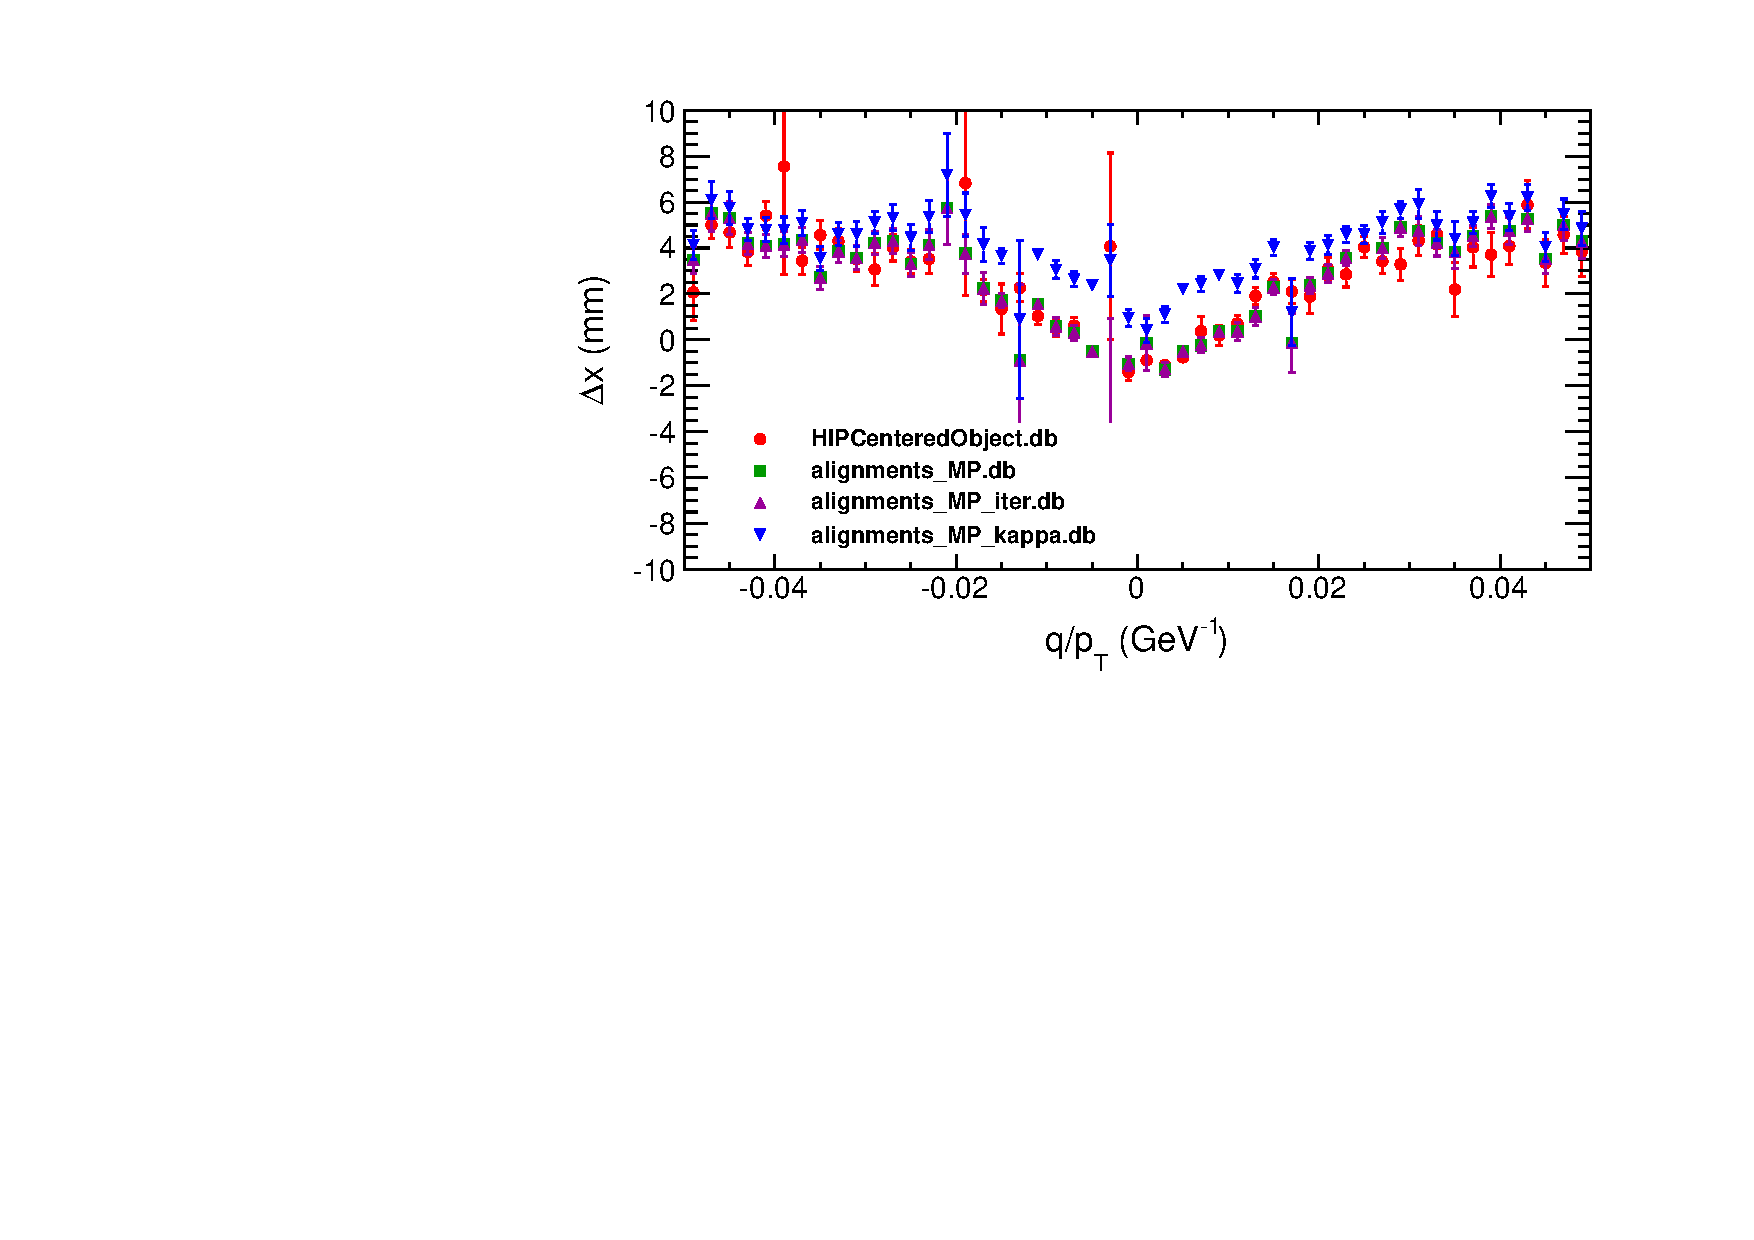
\includegraphics[width=0.9\linewidth]{mptrackeralignments_allthree.pdf}
\end{frame}

\begin{frame}
\frametitle{Beam-halo trigger losing events}

\scriptsize
\begin{itemize}
\item Beam-halo tracks in overlap of neighboring CSCs are selected at HLT in a dedicated trigger, sent to a dedicated AlCa stream
\item Hit pattern used to identify a track parallel to the beamline
  has a broader distribution in later runs (e.g.\ runs with
  $\vec{B}$-field on, not tested in MC)
\item Muons travelling parallel to beam-line would be affected by radial component of $\vec{B}$-field: that could be what is broadening the distribution
\item Working with Joe Gartner (now responsible for this trigger) to fix it
\end{itemize}

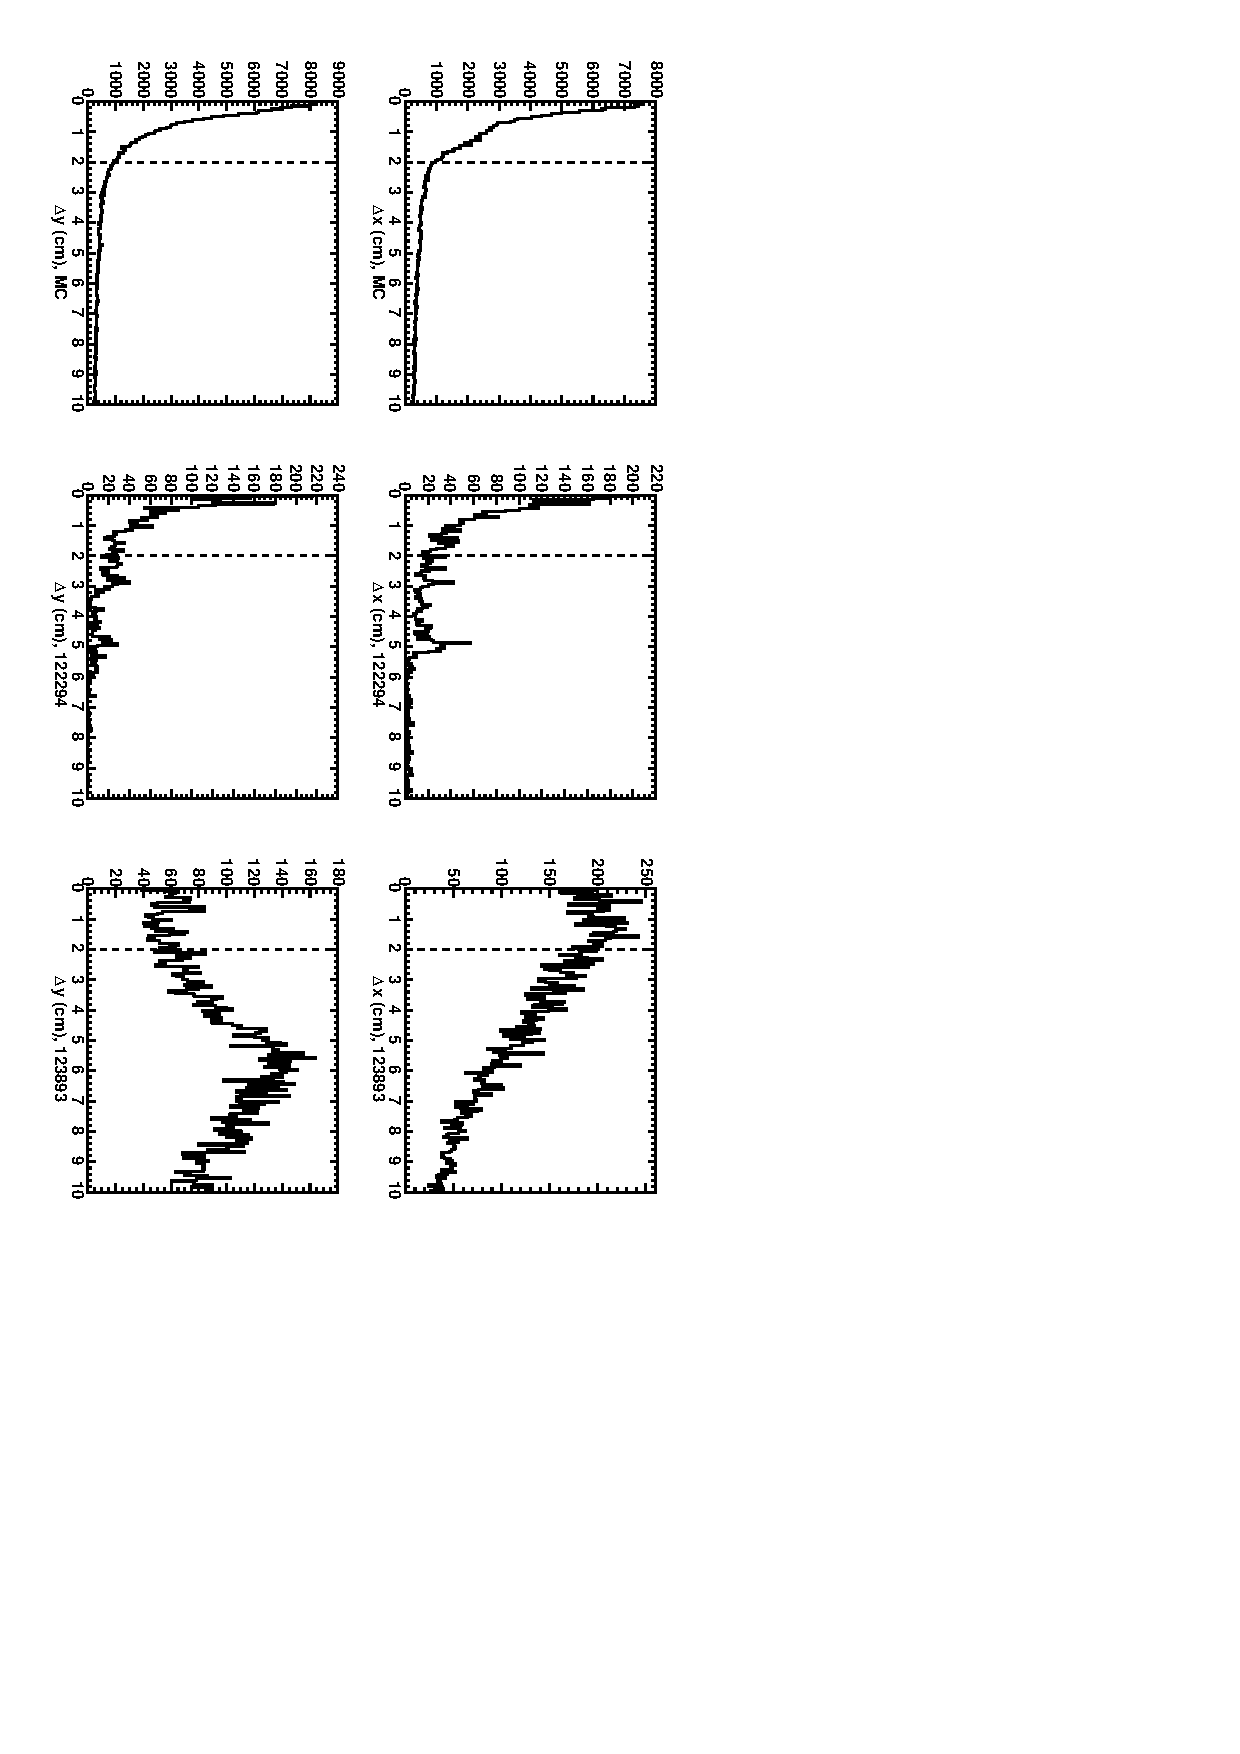
\includegraphics[height=0.9\linewidth, angle=90]{HLT_CSCBeamHaloOverlaps.pdf}

\end{frame}

\begin{frame}
\frametitle{Work-around}

\scriptsize
\begin{itemize}
\item We built in a work-around: another trigger and another AlCa stream that don't select overlaps
\item Reprocessed this stream without the faulty HLT algorithm
\item Still far too few beam-halo muons for alignment (we didn't {\it
  lose} an opportunity to align, but we learned something important
  about our trigger so that we don't lose anything in the future)
\item First example plot: $dR/dz$ for identifying beam-halo amid the cosmic rays
\end{itemize}

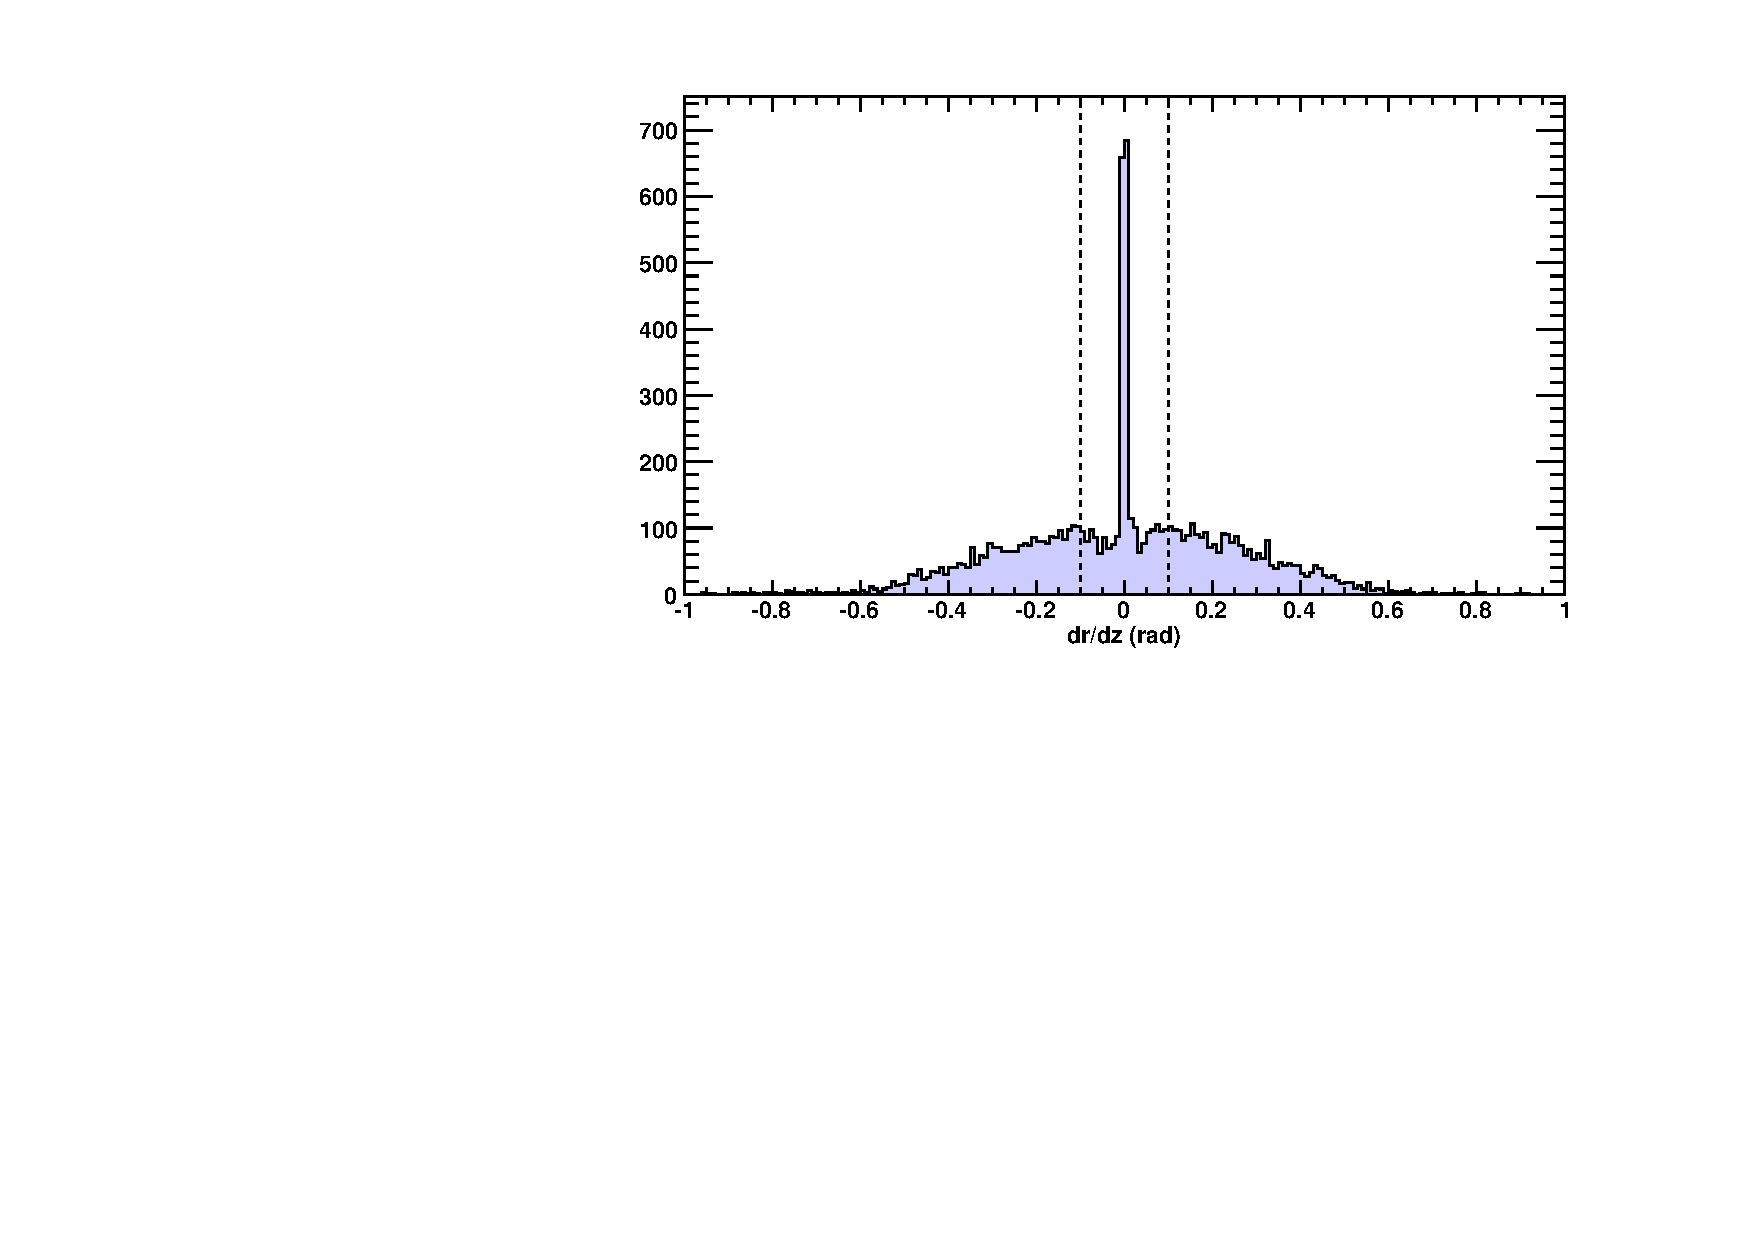
\includegraphics[width=0.8\linewidth]{correctedinput_drdz.pdf}
\end{frame}

\begin{frame}
\frametitle{Occupancy by station/ring}

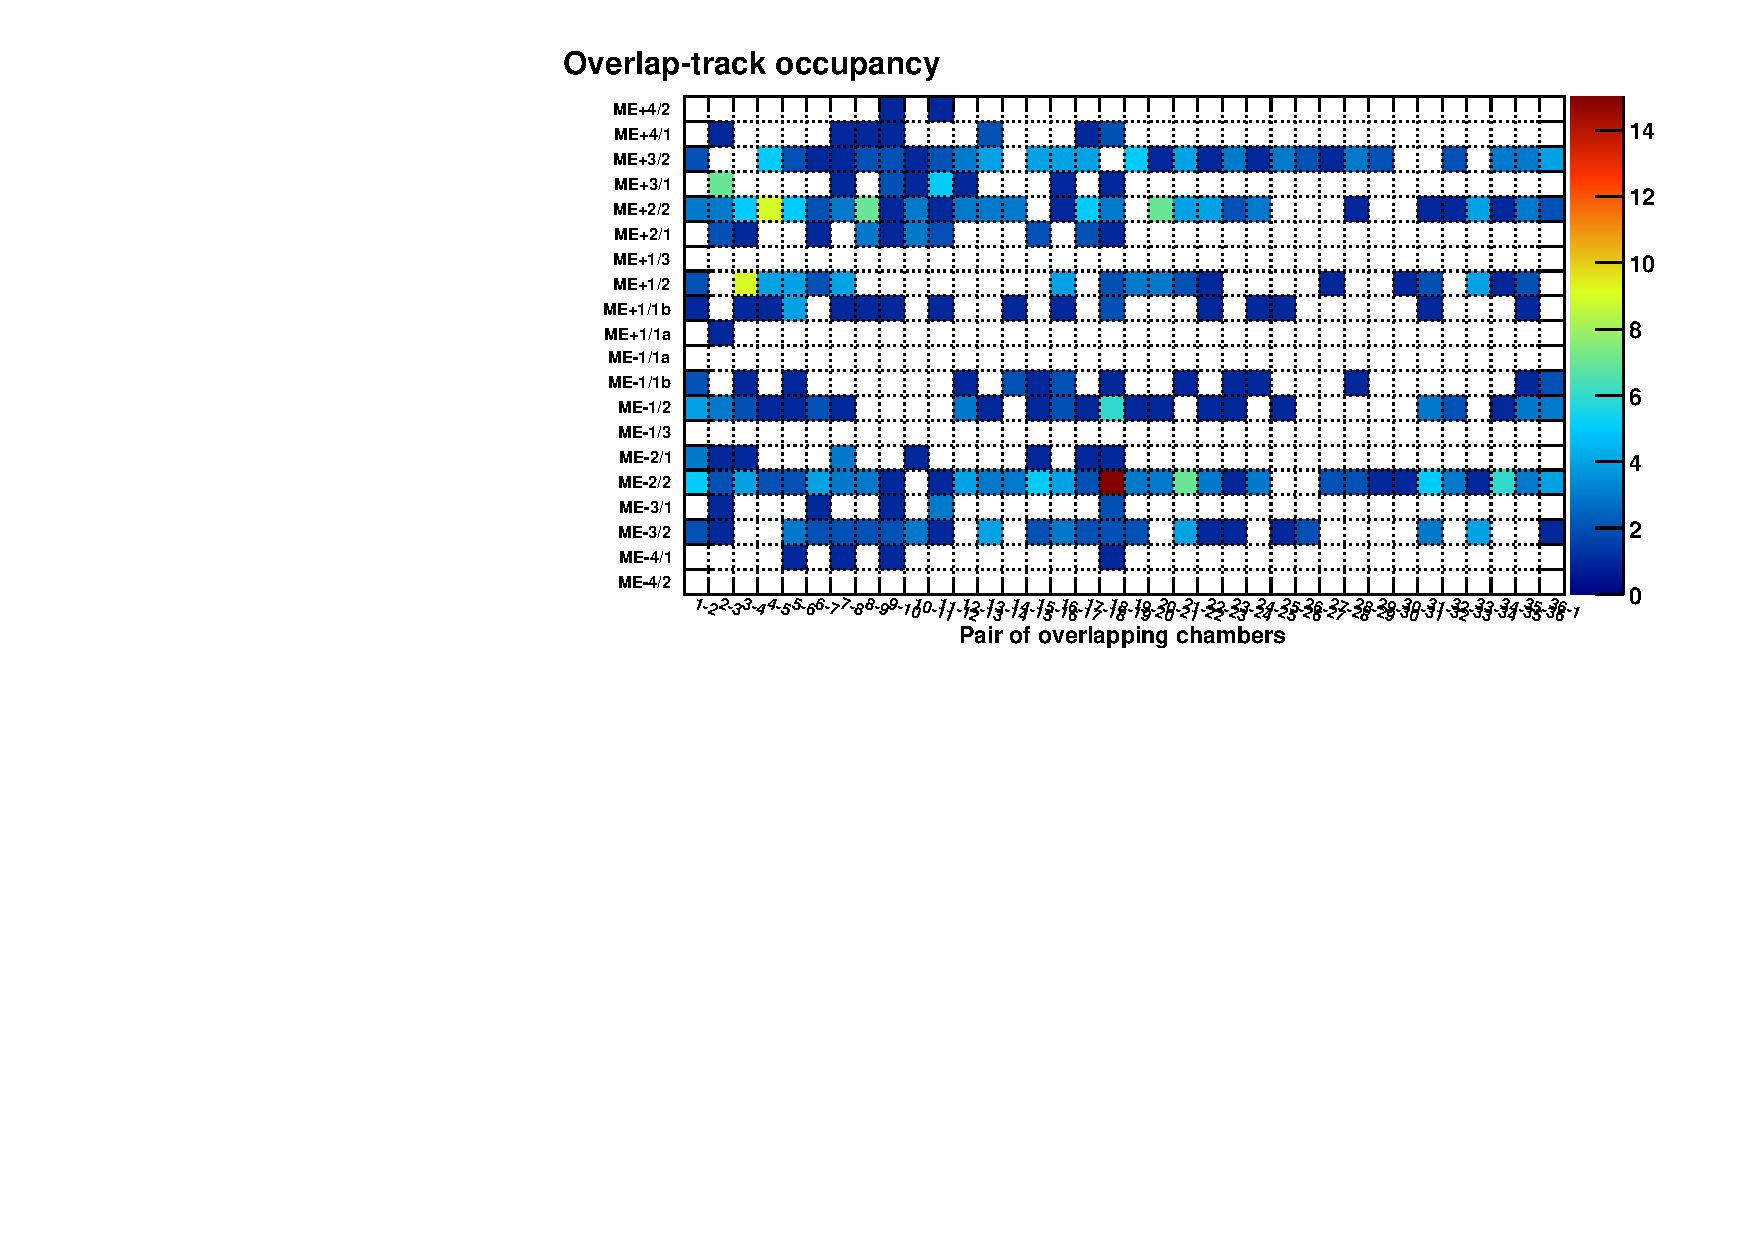
\includegraphics[width=\linewidth]{correctedinput_occupancy.pdf}
\end{frame}

\begin{frame}
\frametitle{Hit distribution: global $x$-$y$}

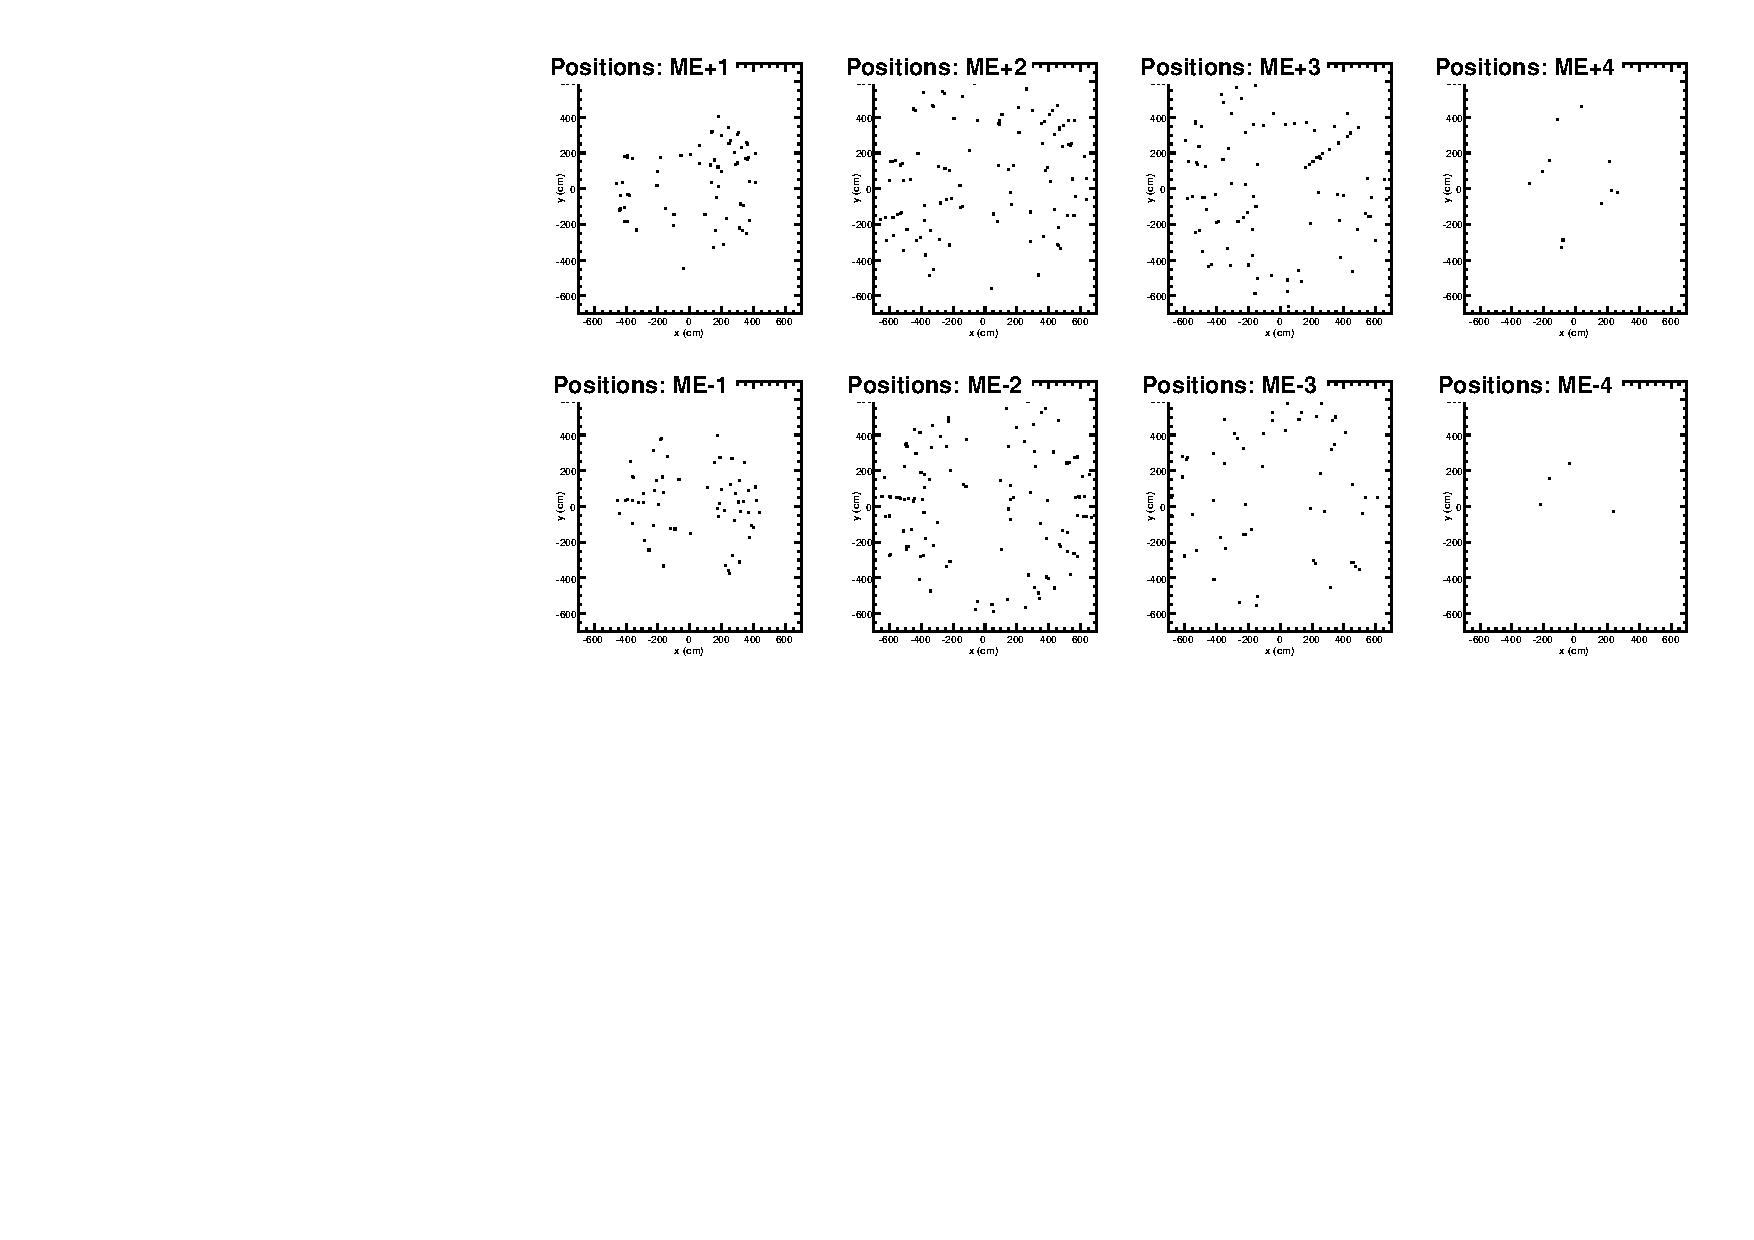
\includegraphics[width=\linewidth]{correctedinput_xypos.pdf}
\end{frame}

\begin{frame}
\frametitle{Hit distribution: $r$-$\phi$}

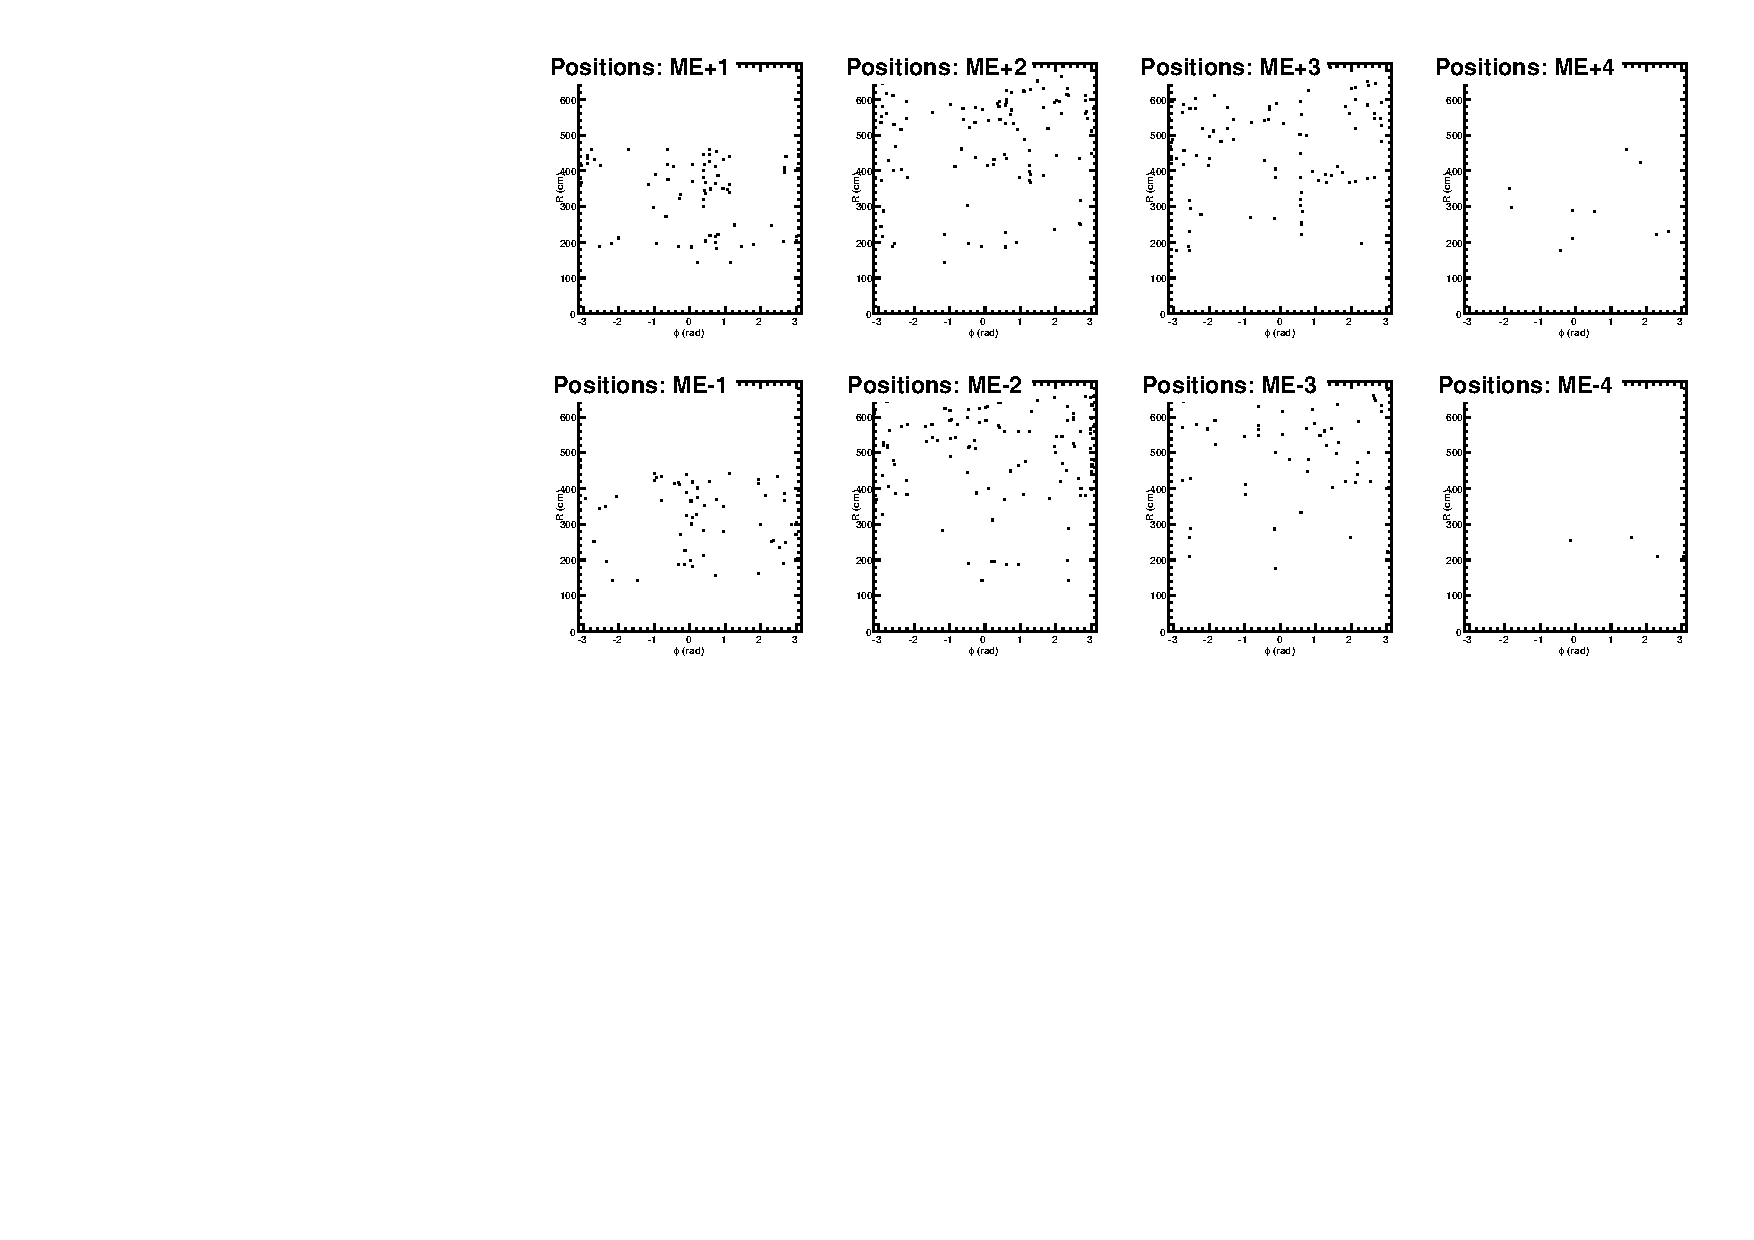
\includegraphics[width=\linewidth]{correctedinput_rphipos.pdf}
\end{frame}

\begin{frame}
\frametitle{Analysis}

\scriptsize
\begin{itemize}
\item Read Alfredo's e-mail, and walked through the process of skimming and PATifying a sample
\item Aysen did this on his own, too
\item I optimized a set of keep statements for our purposes:
\begin{itemize}
\item \scriptsize all generator-level information, including SimHits (which are big; we could save a lot by dropping these)
\item \scriptsize PAT muons and also RECO muons, including muons made with the SET algorithm
\item \scriptsize all tracks and the hits attached to tracks: a trick learned from AlCaRecos (we can refit tracks if needed)
\item \scriptsize all muon hits
\item \scriptsize enough calorimetry to re-run isolation, so that we can make isolation algorithms of any level of sophistication
\item \scriptsize beamspot, primary vertices, trigger data, which were essential in real-data exercises with prompt RECO
\item \scriptsize tested all of the above with the output, including calculation of MC weights (for PDF systematics studies) and event display
\end{itemize}
\item Background skims of $p_{T1} > 20$~GeV, $p_{T2} > 5$~GeV are tight: we can make them looser
\end{itemize}
\end{frame}

\begin{frame}
\frametitle{Important warning}

\begin{itemize}
\item PAT muons are a union of globalMuons, trackerMuons (tracker-track plus one or more segments), and standAloneMuons
\item standAloneMuons are not useful for our analysis (too-loose identification and poor resolution)
\item We'll want to control which algos we use: e.g.\ globalMuon-globalMuon, globalMuon-trackerMuon, trackerMuon-trackerMuon
\end{itemize}

\vspace{0.5 cm}
\hspace{-0.83 cm} \textcolor{darkblue}{\Large Location of samples}
\begin{itemize}
\item Signal: we generate that at Fermilab
\item $pp \to \mu X$: available at Fermilab and CERN (use Fermilab)
\item For the others: need CRAB access, should get Aysen set up with an account
\begin{itemize}
\item just use CRAB to get a skim, then we work with the skim locally
\end{itemize}
\end{itemize}
\end{frame}

\begin{frame}
\frametitle{Mass vs.\ $R$}

\begin{itemize}
\item These are just any pair of muons (6 pairs per 4-muon event): I'm not intending to reproduce Aysen's work!  Just to check the samples and learn some things about what PAT provides
\item Wrong combinations generally have high mass
\item Signal always on left, background always on right
\end{itemize}

\begin{columns}
\column{0.5\linewidth}
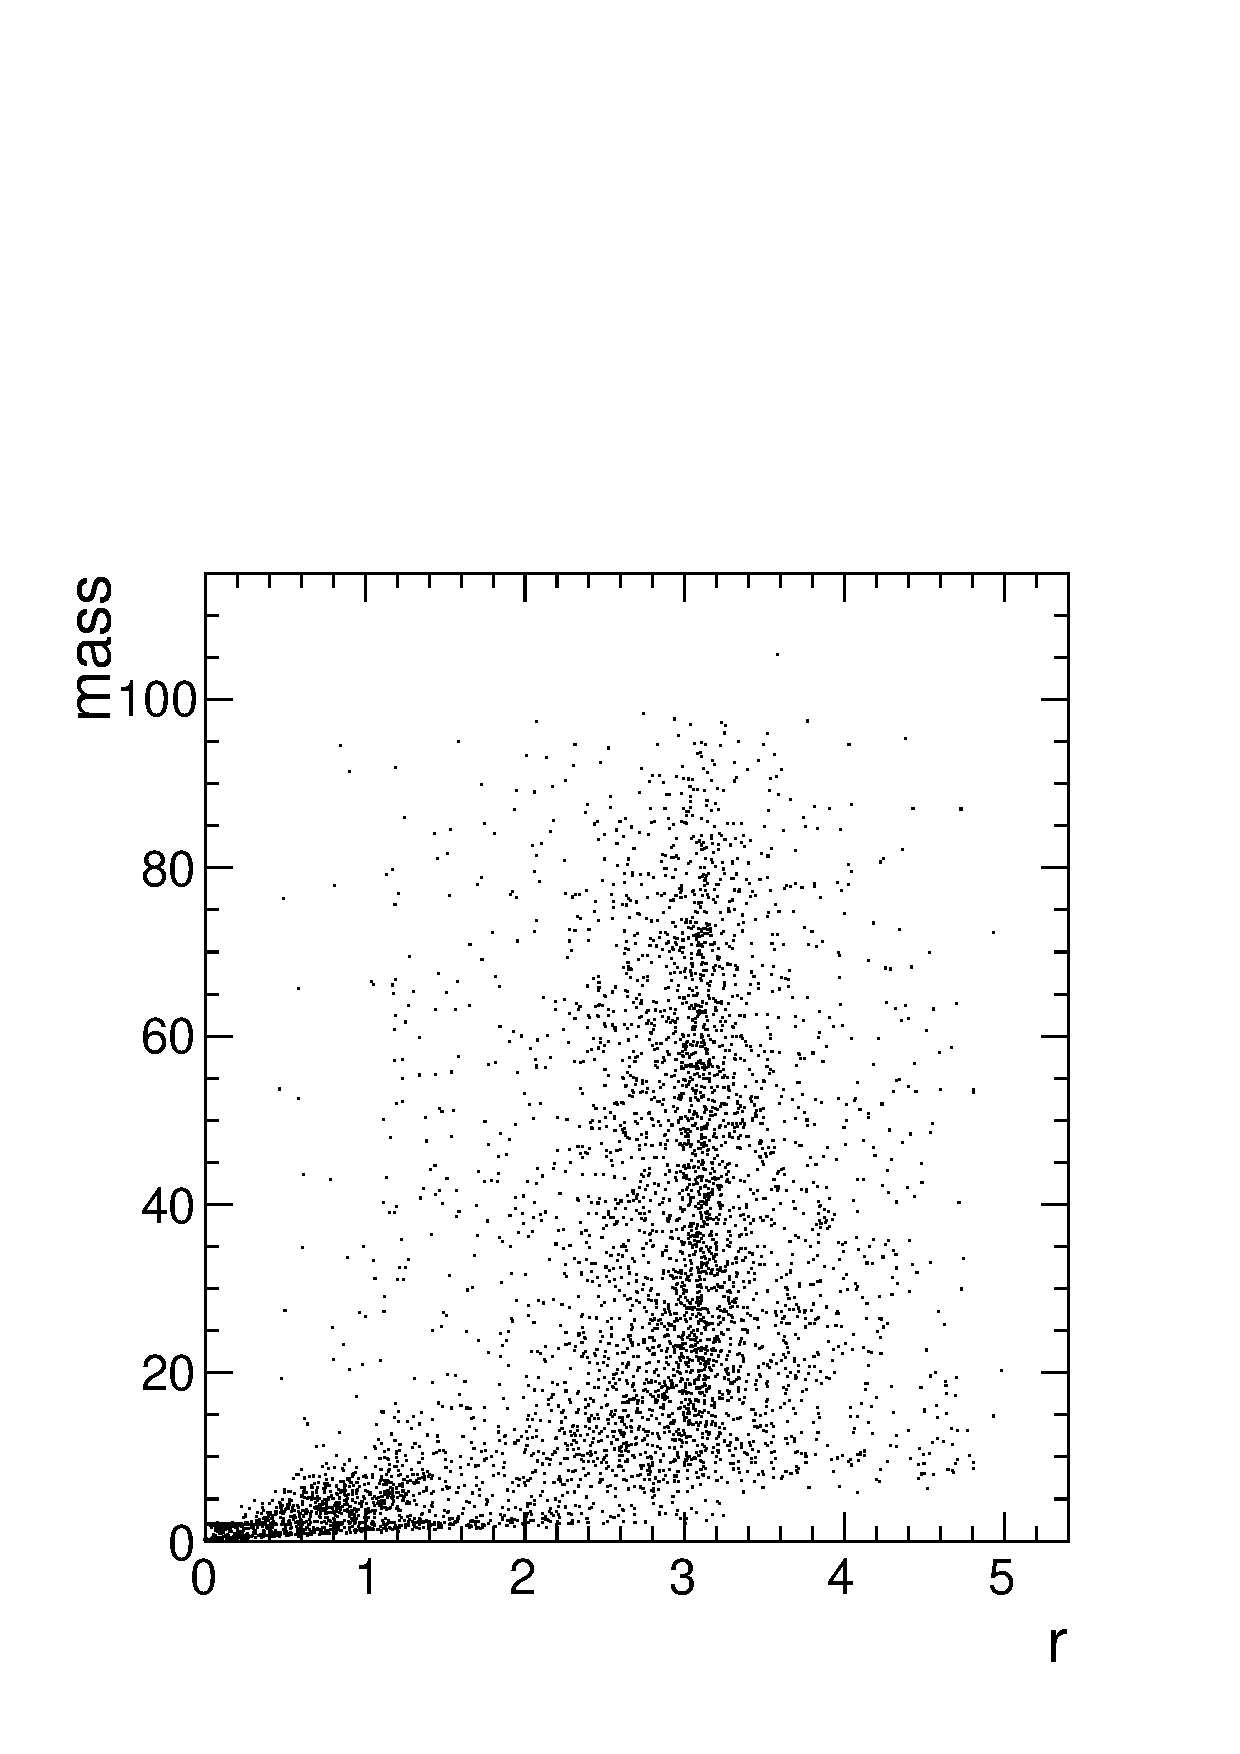
\includegraphics[width=\linewidth]{mass_vs_r.pdf}
\column{0.5\linewidth}
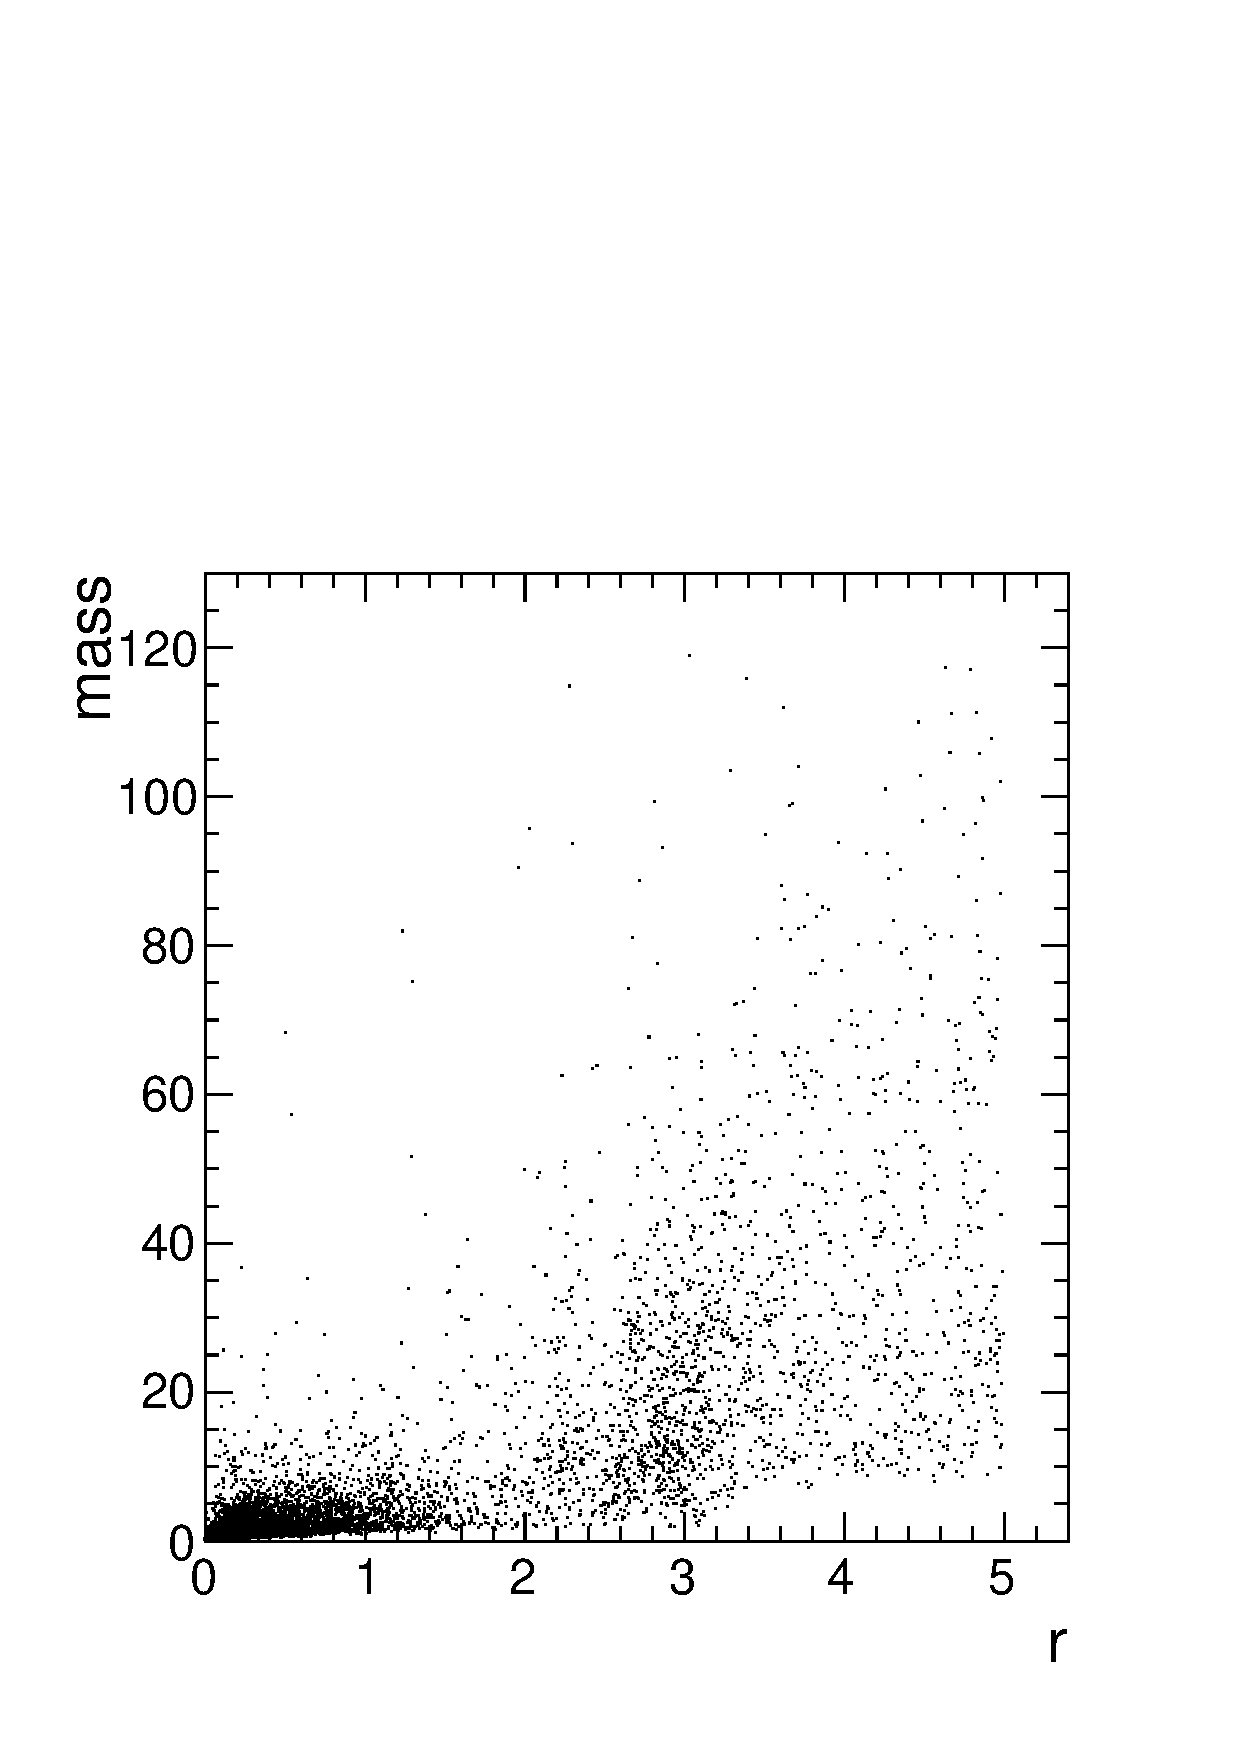
\includegraphics[width=\linewidth]{mass_vs_r_background.pdf}
\end{columns}
\end{frame}

\begin{frame}
\frametitle{Mass vs.\ $R$}

\begin{itemize}
\item Zoom in
\end{itemize}

\begin{columns}
\column{0.5\linewidth}
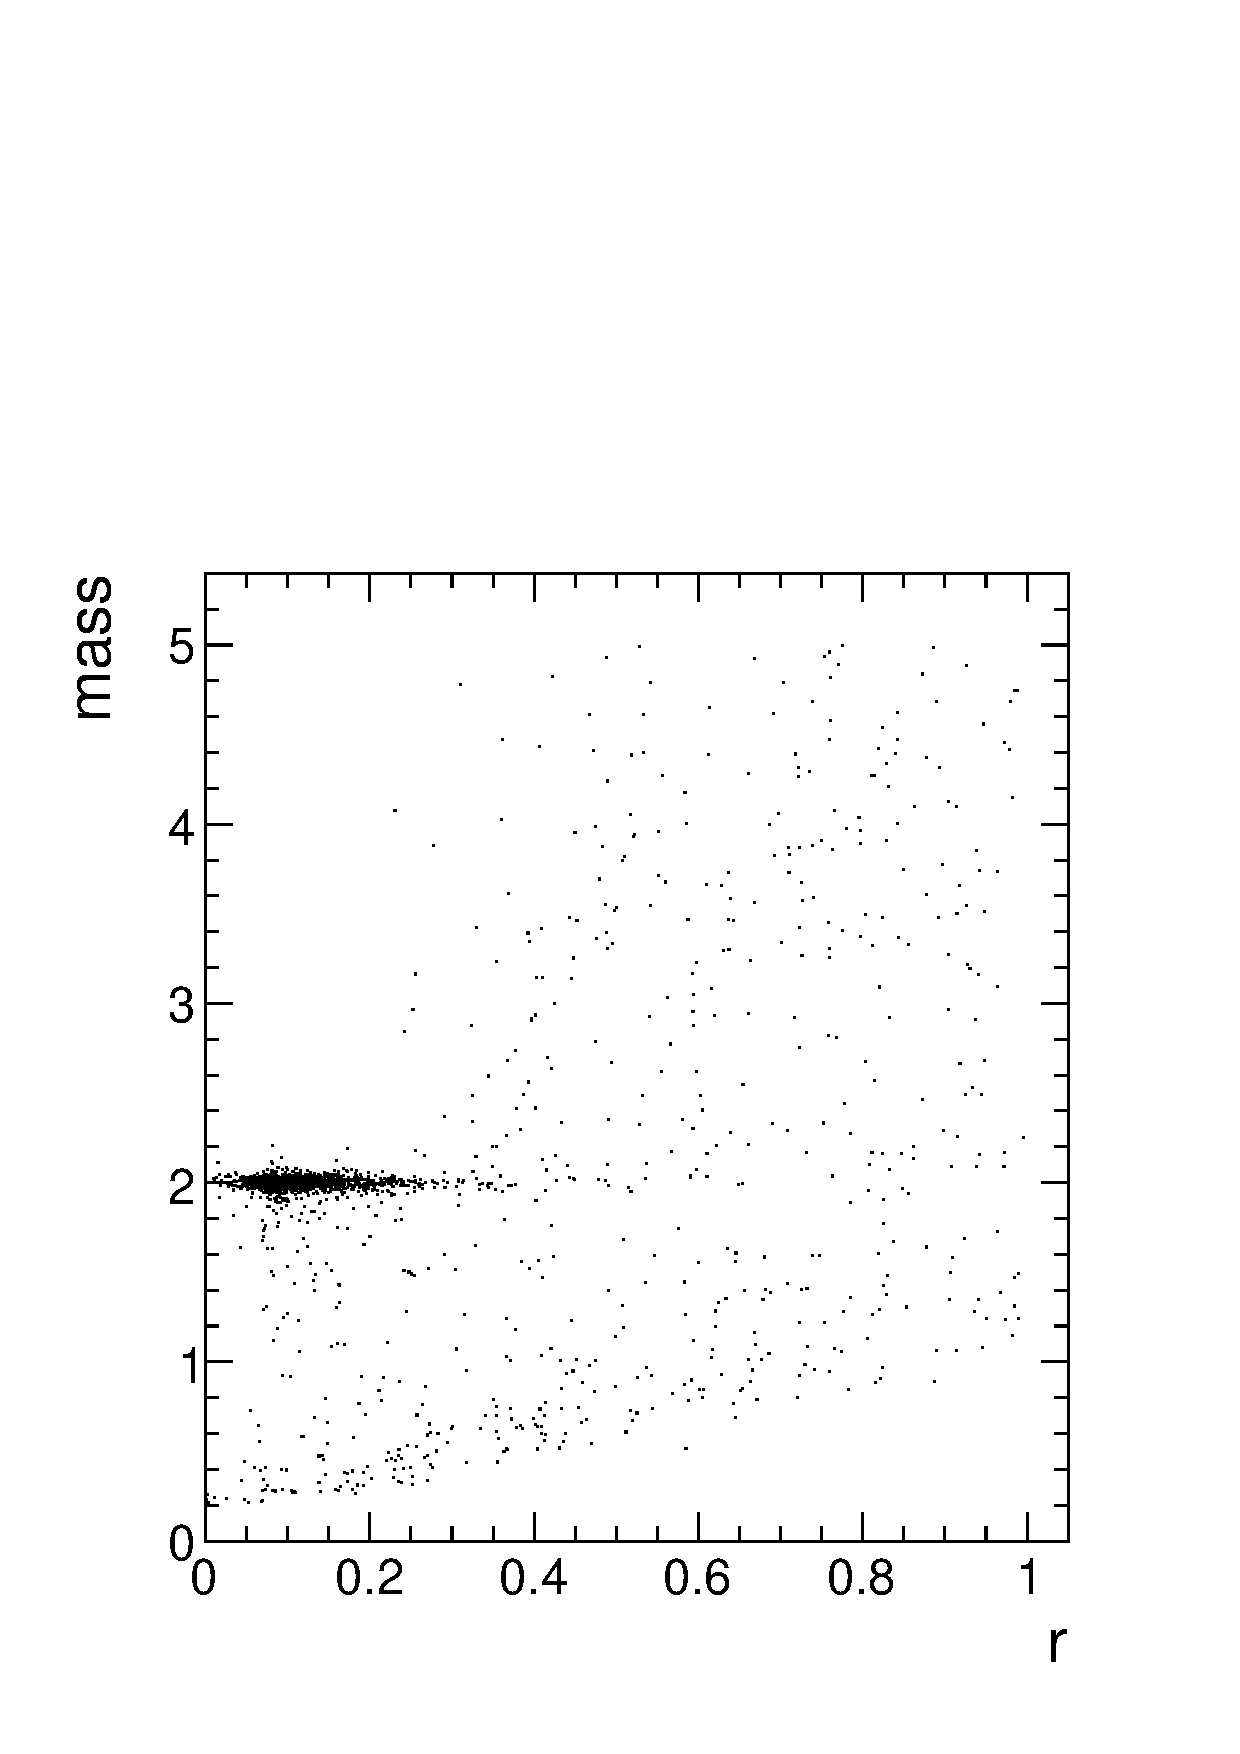
\includegraphics[width=\linewidth]{mass_vs_r2.pdf}
\column{0.5\linewidth}
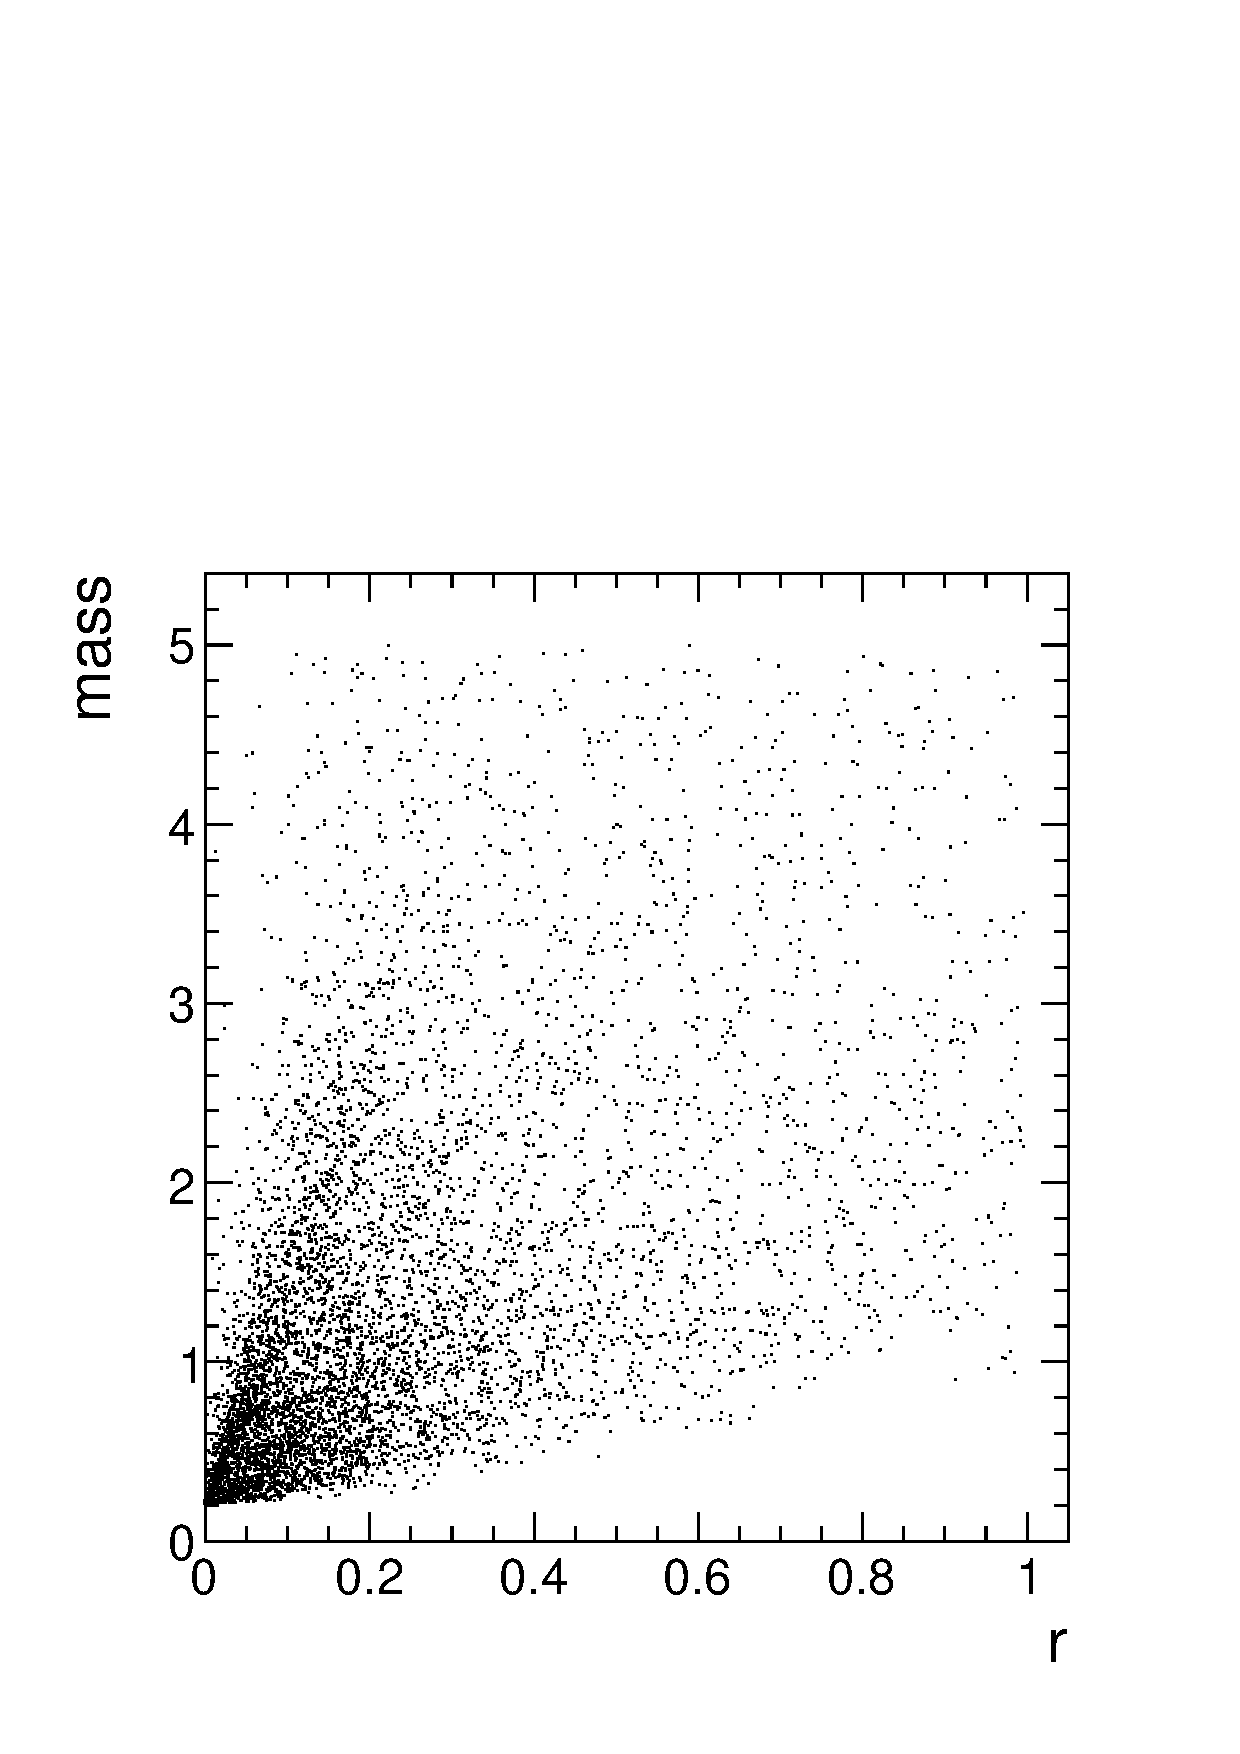
\includegraphics[width=\linewidth]{mass_vs_r2_background.pdf}
\end{columns}
\end{frame}

\begin{frame}
\frametitle{Mass distribution}

\begin{itemize}
\item No clean-up, just a raw look at the data
\end{itemize}

\begin{columns}
\column{0.5\linewidth}
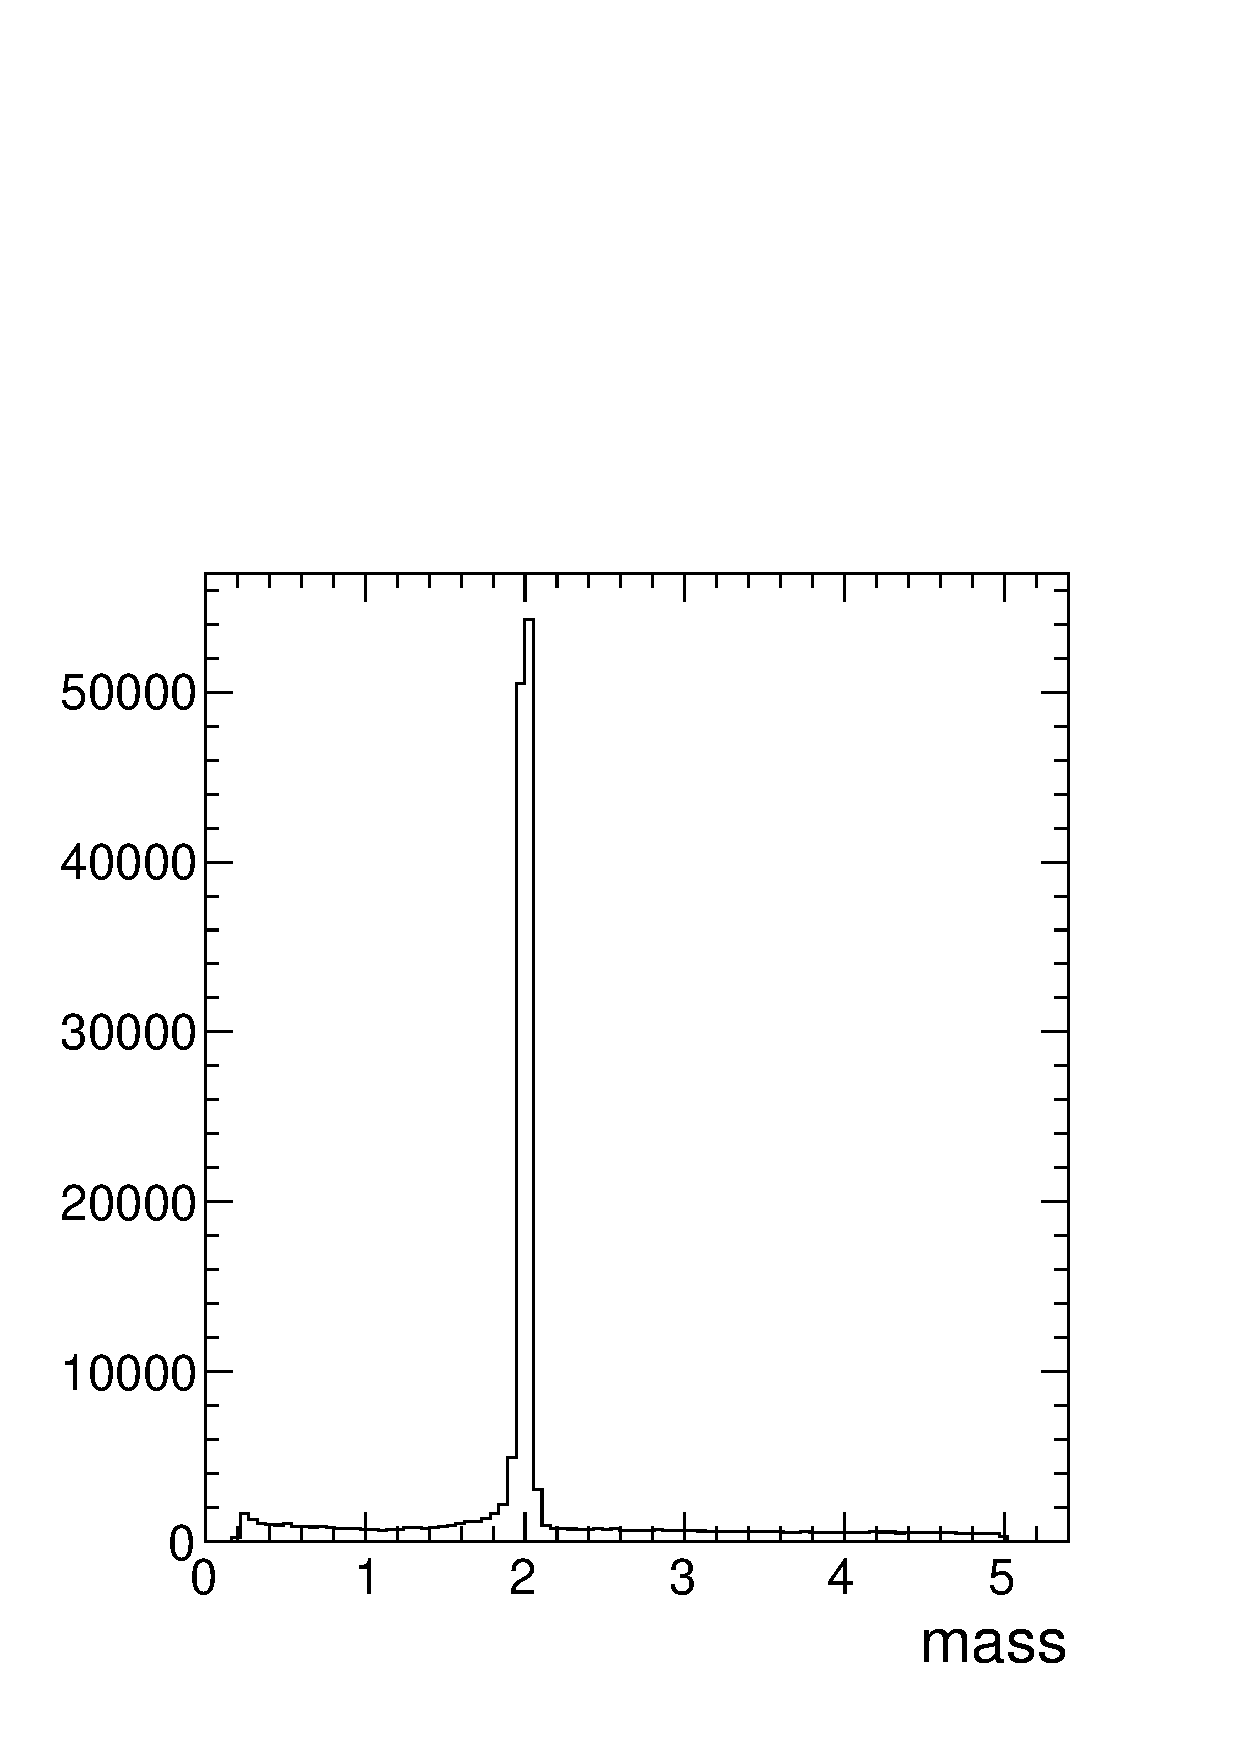
\includegraphics[width=\linewidth]{mass.pdf}
\column{0.5\linewidth}
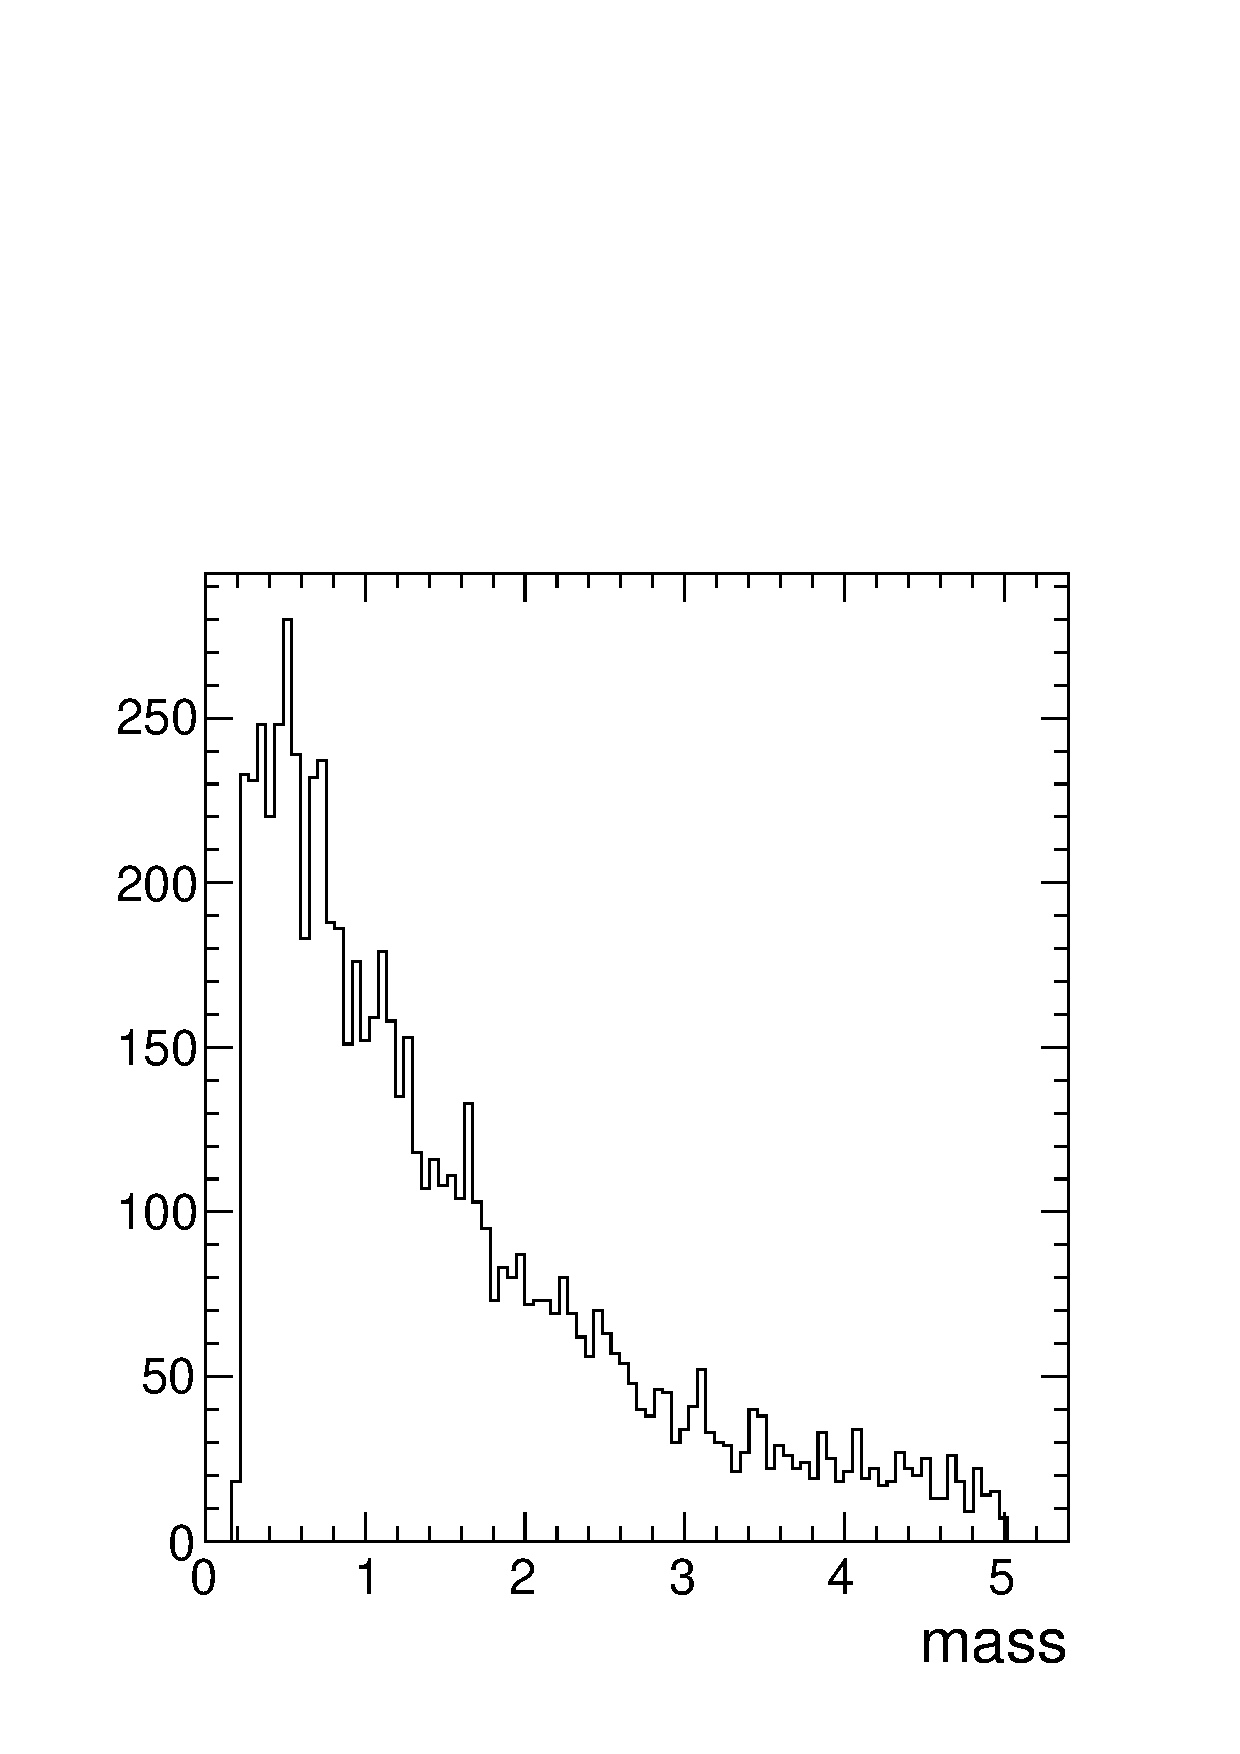
\includegraphics[width=\linewidth]{mass_background.pdf}
\end{columns}
\end{frame}

\begin{frame}
\frametitle{MC matches}

\begin{itemize}
\item PAT matches reconstructed muons to generator-level muons for free
\item Remember that backgrounds have a lower $p_T$ spectrum
\end{itemize}

\begin{columns}
\column{0.5\linewidth}
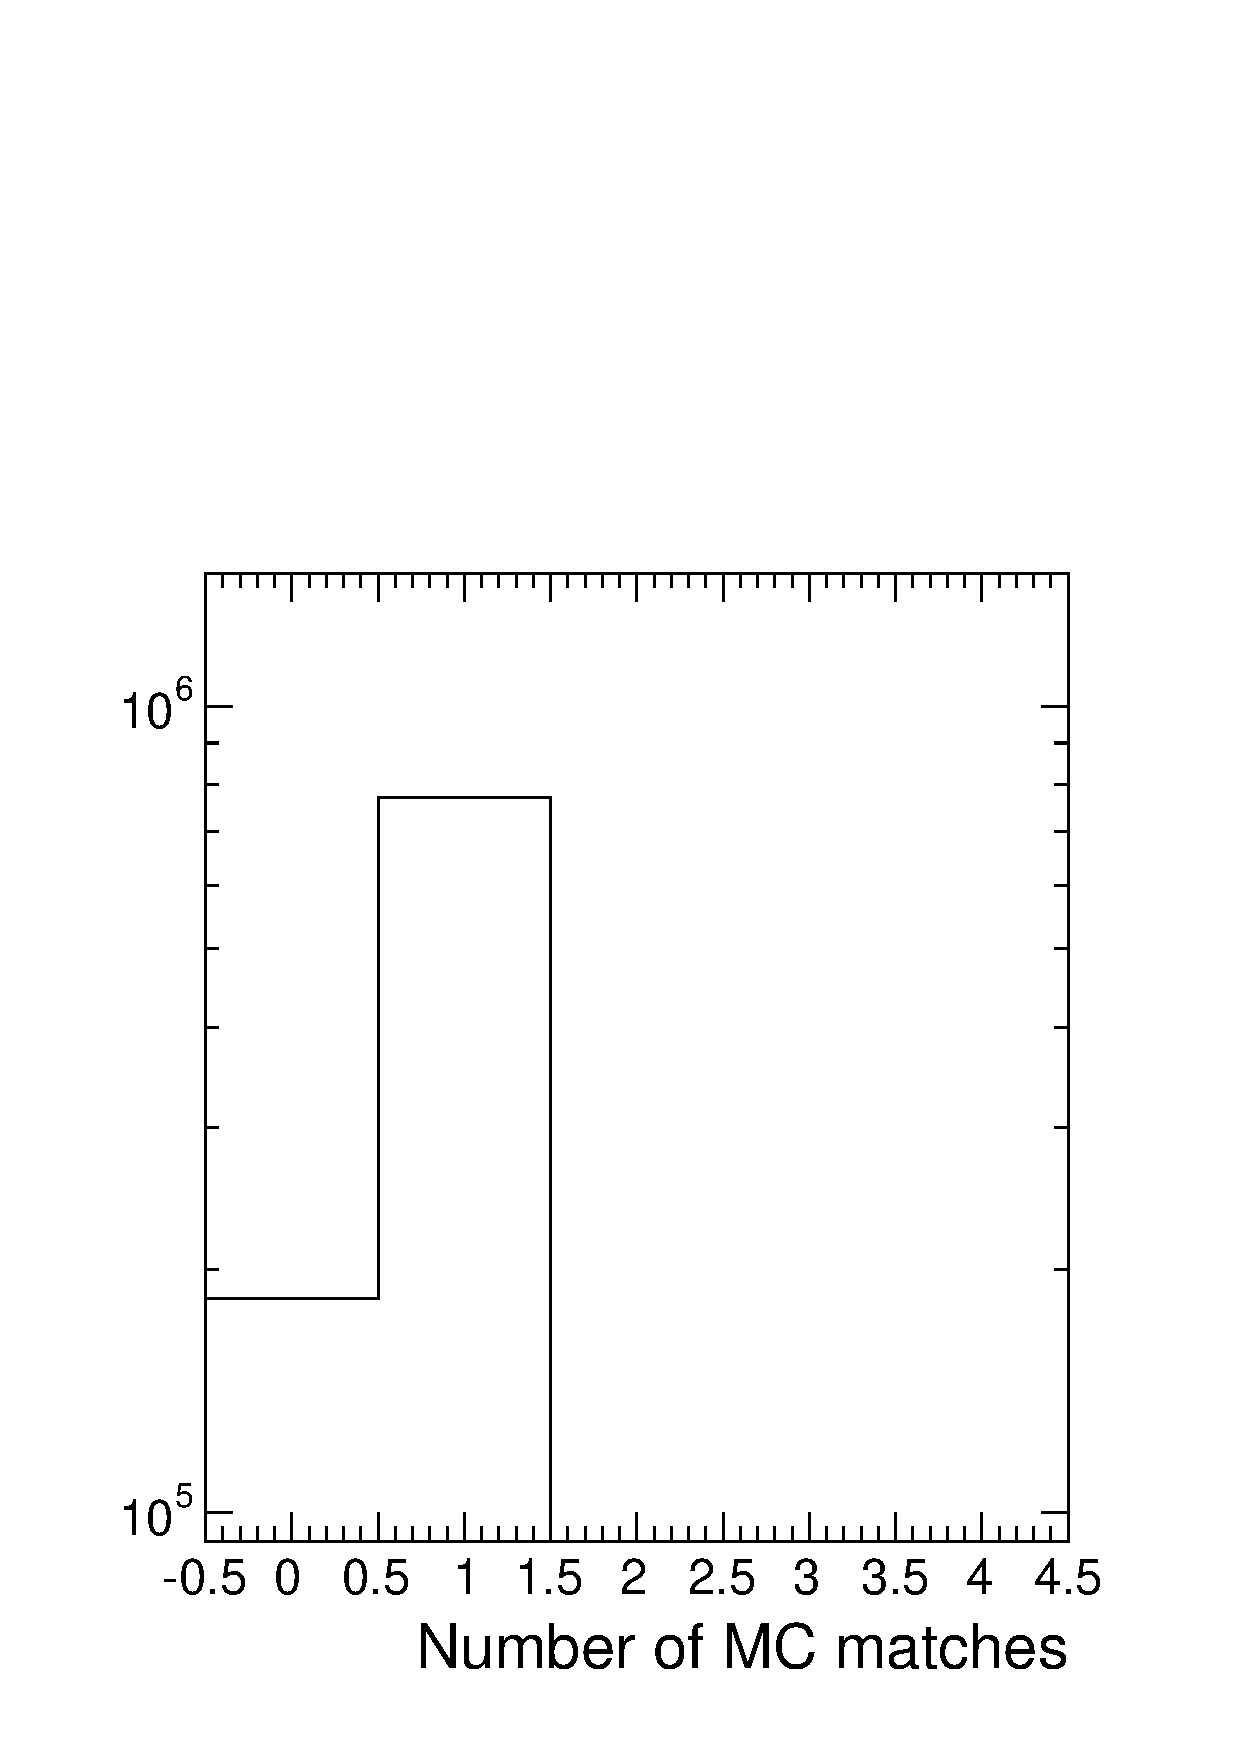
\includegraphics[width=\linewidth]{nummatches.pdf}
\column{0.5\linewidth}
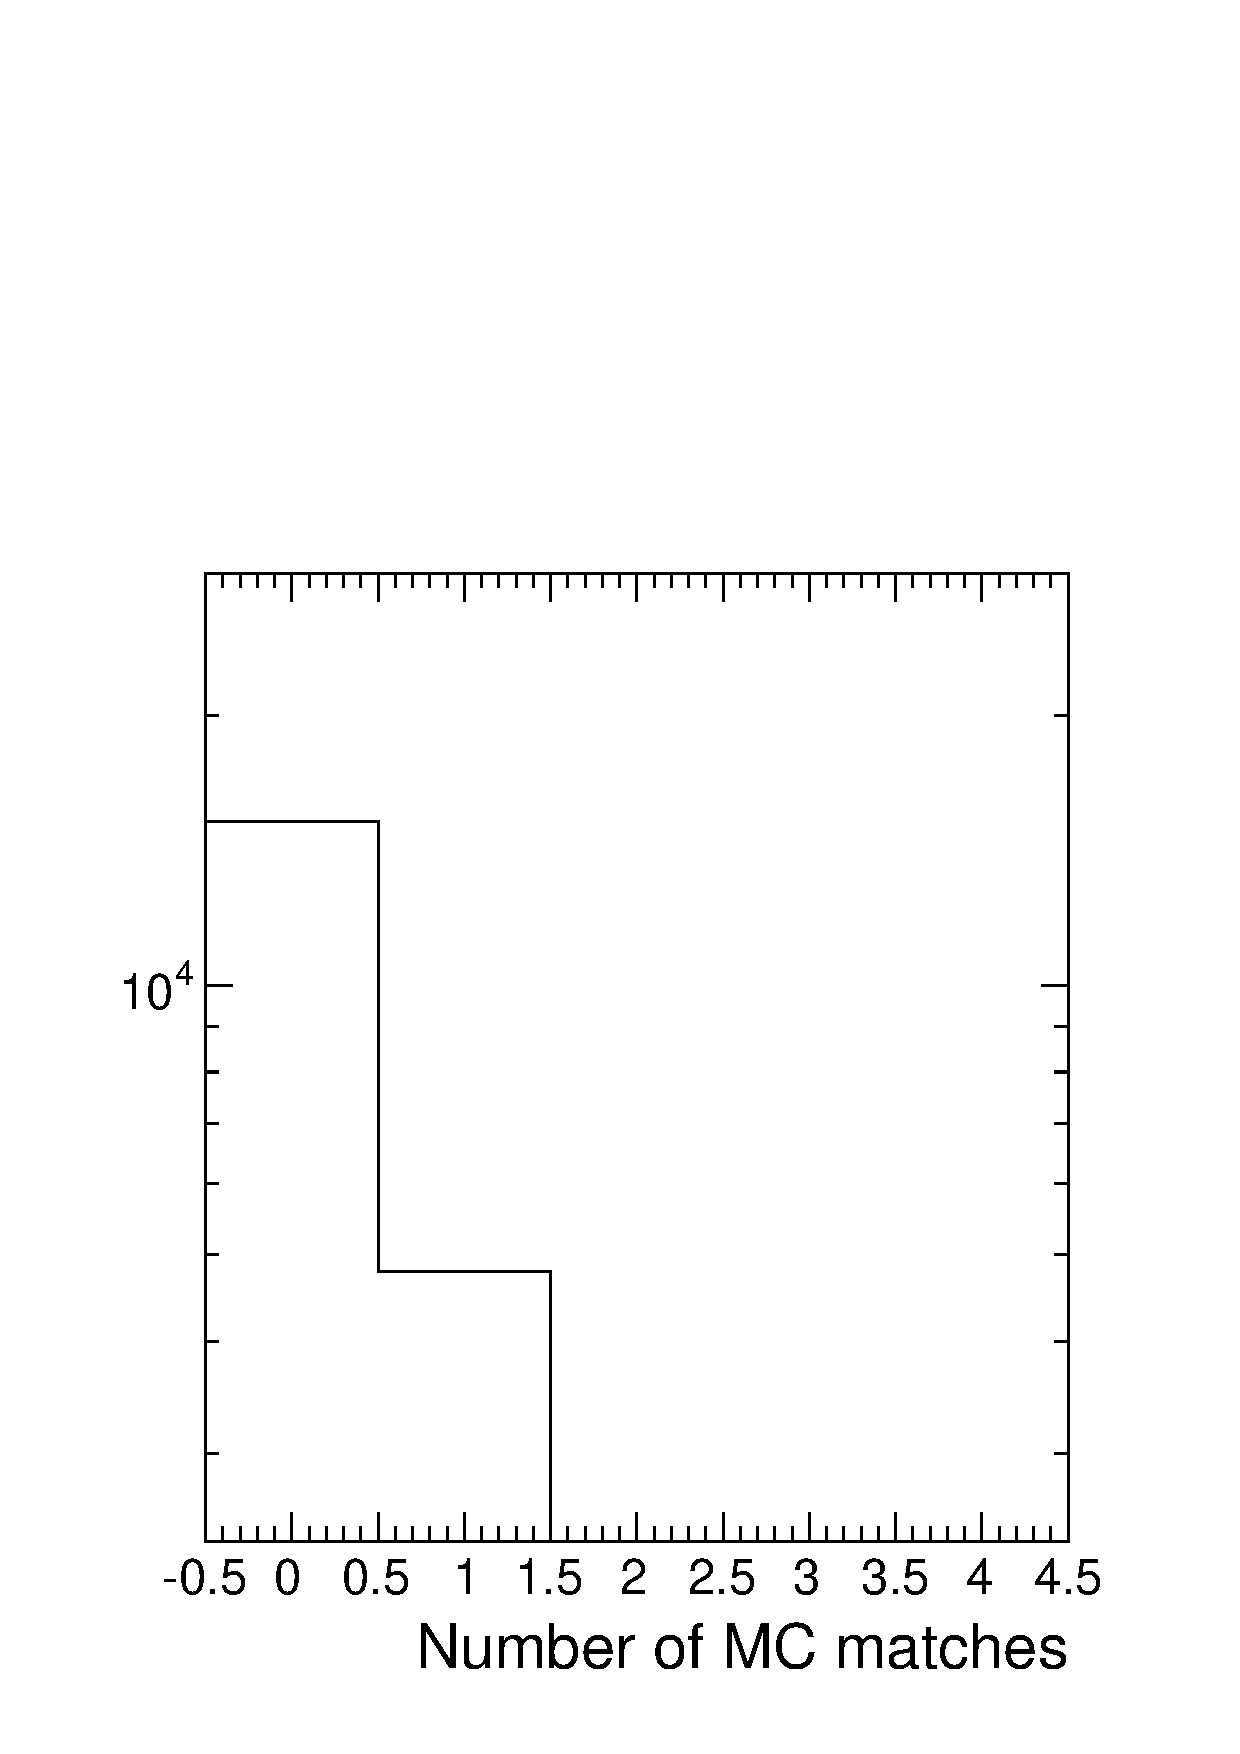
\includegraphics[width=\linewidth]{nummatches_background.pdf}
\end{columns}
\end{frame}

\begin{frame}
\frametitle{PDG-id of parent}

\begin{itemize}
\item Most signal muons come from $a_1$ (PDG-id = 36)
\item The rest (signal and background) are from charm and bottom
  mesons (PDG-ids in the 100's) and baryons (PDG-ids in the 1000's)
\end{itemize}

\begin{columns}
\column{0.5\linewidth}
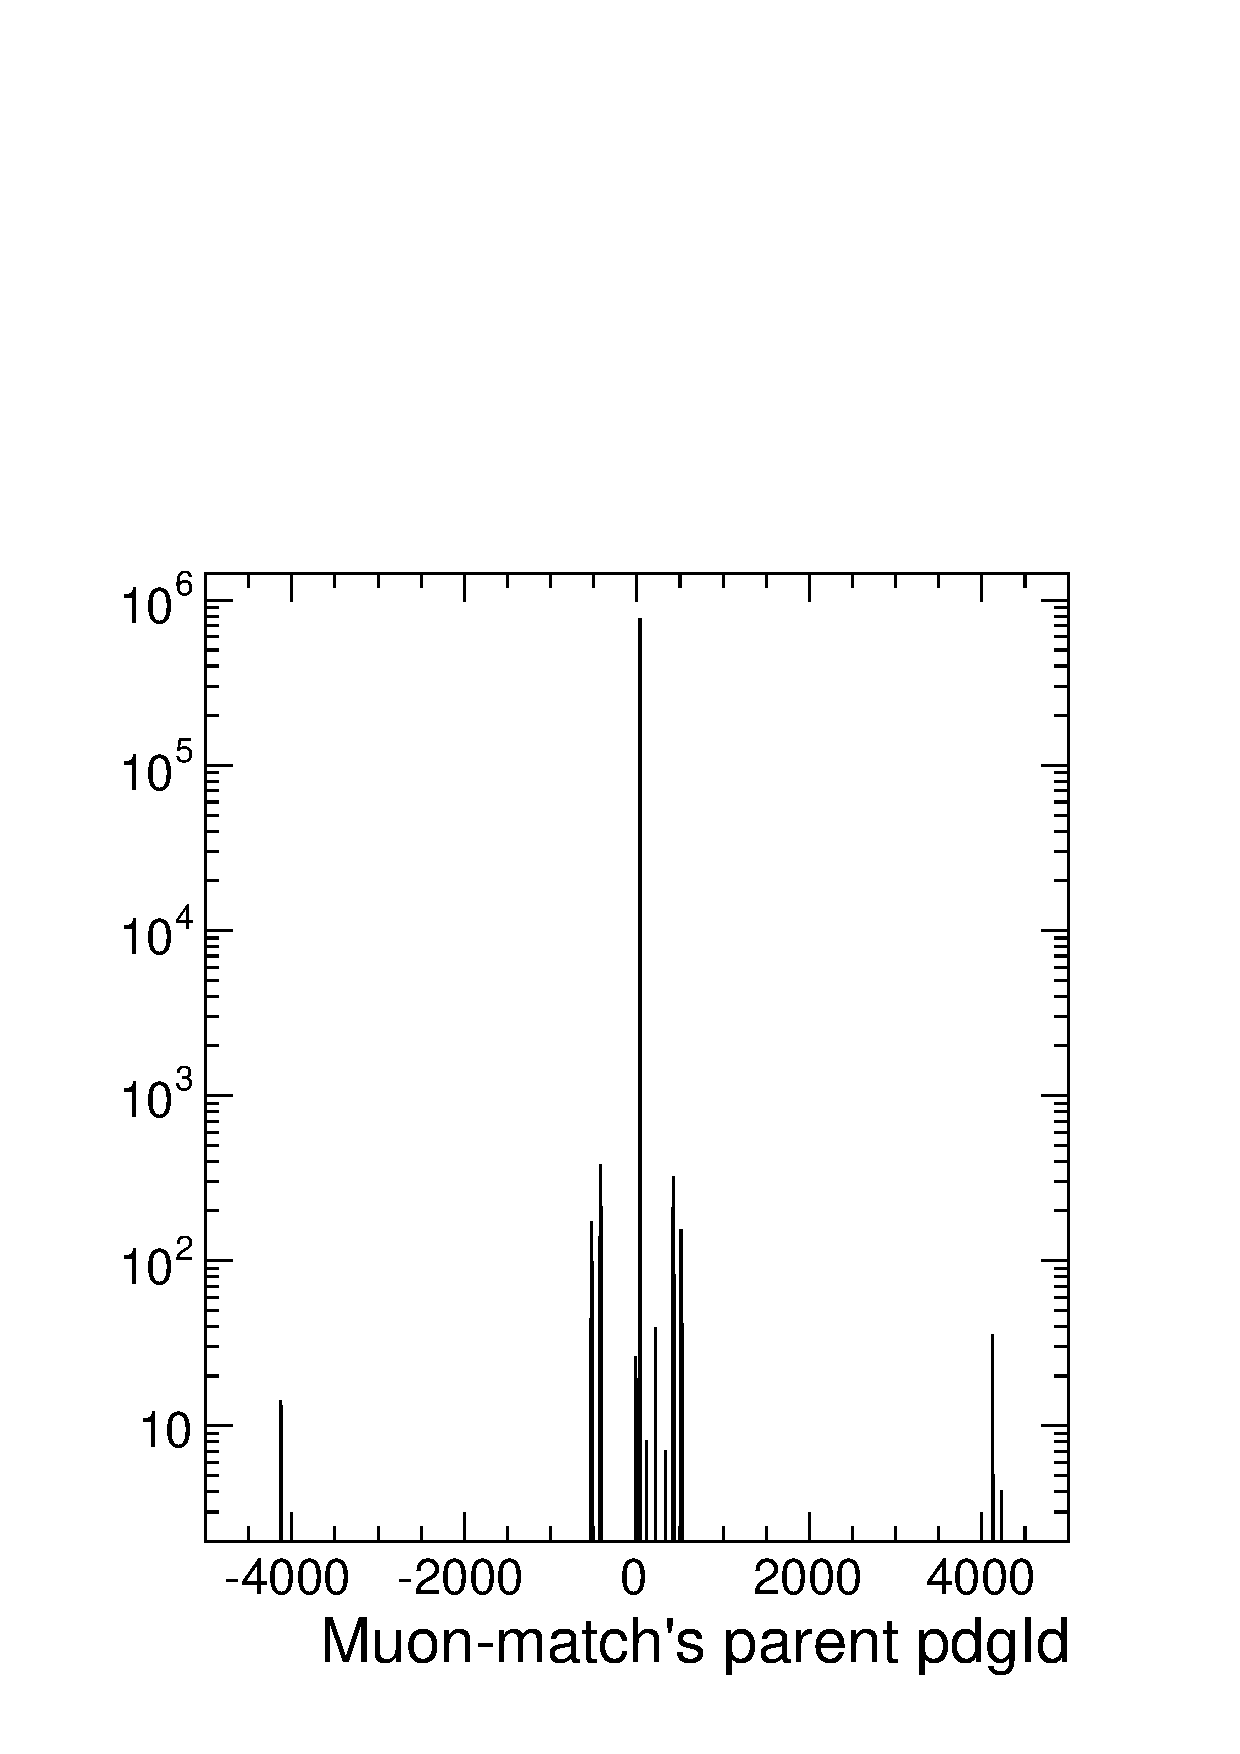
\includegraphics[width=\linewidth]{parents.pdf}
\column{0.5\linewidth}
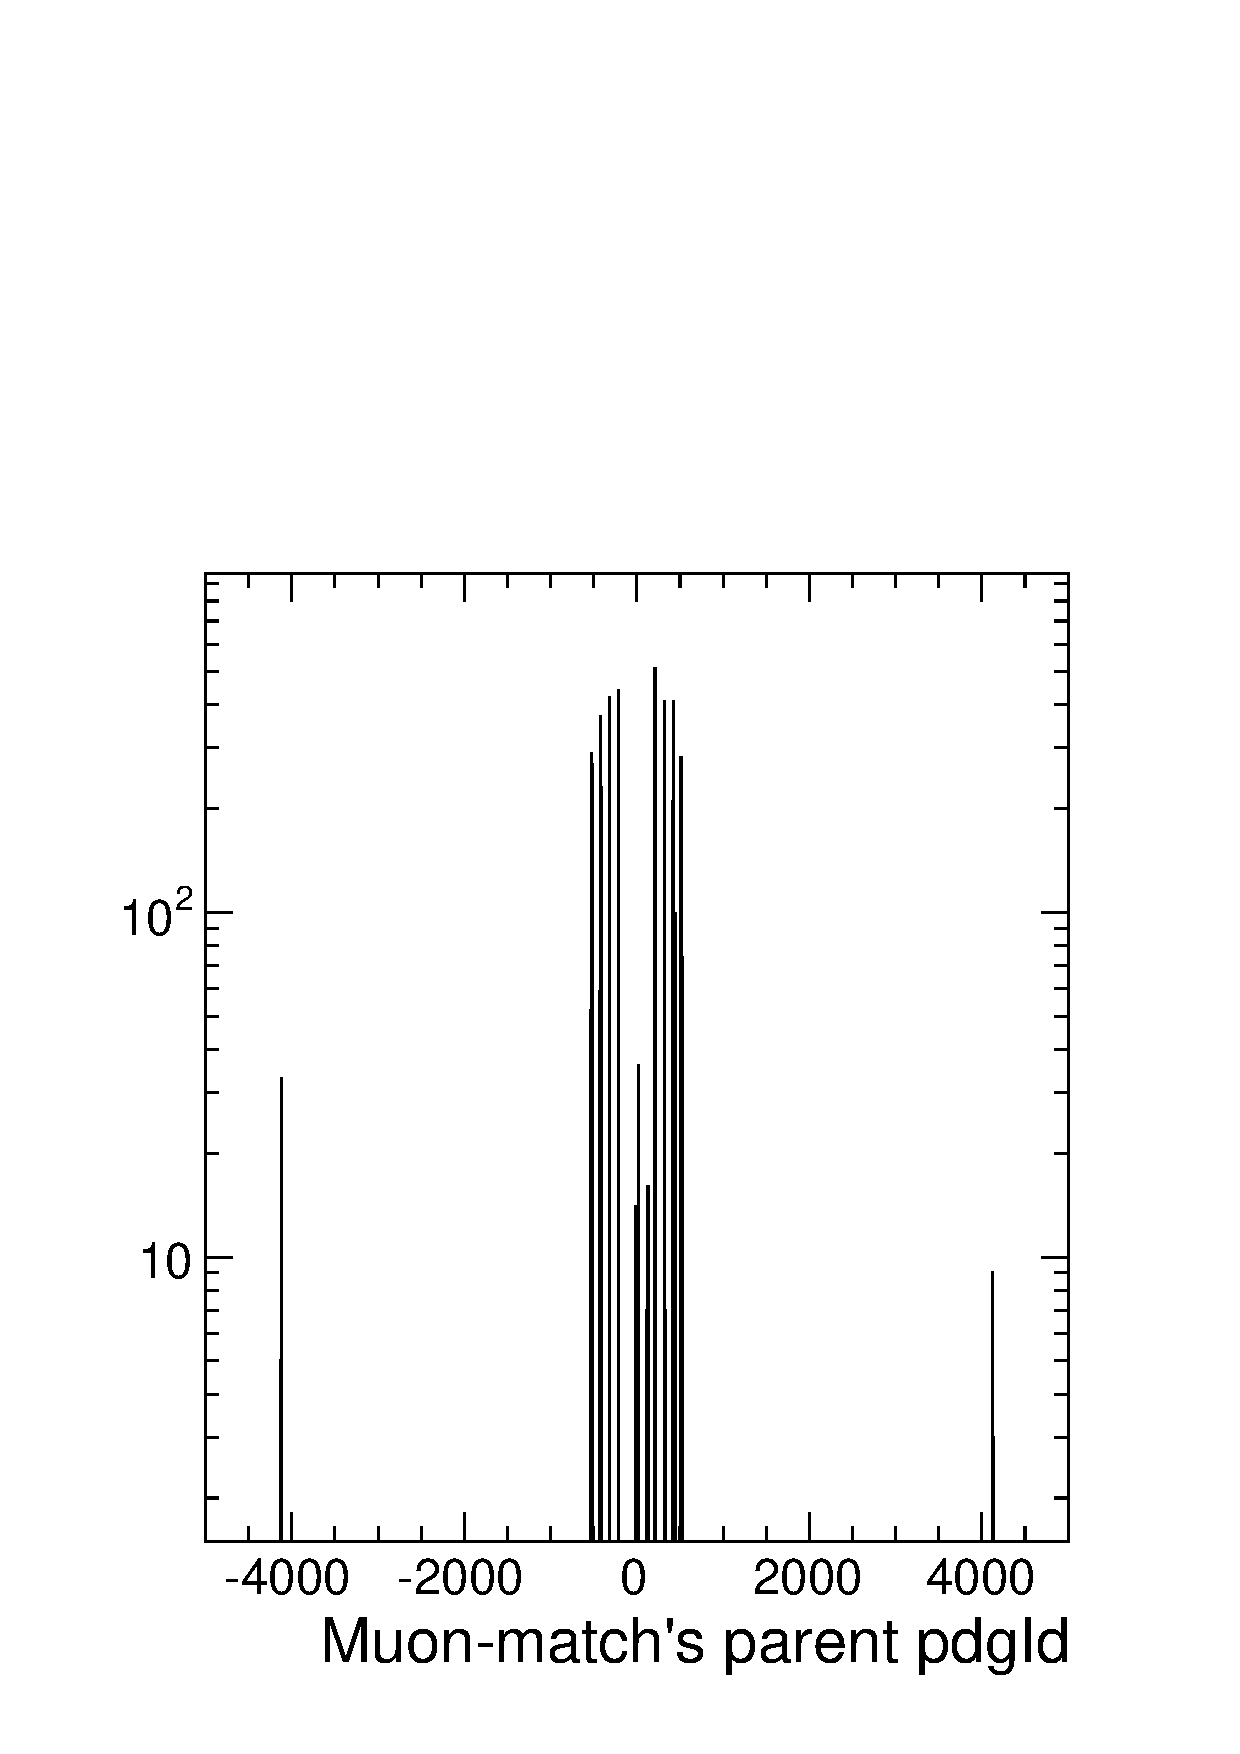
\includegraphics[width=\linewidth]{parents_background.pdf}
\end{columns}
\end{frame}

\begin{frame}
\frametitle{Matched muon $\Delta \phi$}

\begin{itemize}
\item These matches seem pretty reasonable
\end{itemize}

\begin{columns}
\column{0.5\linewidth}
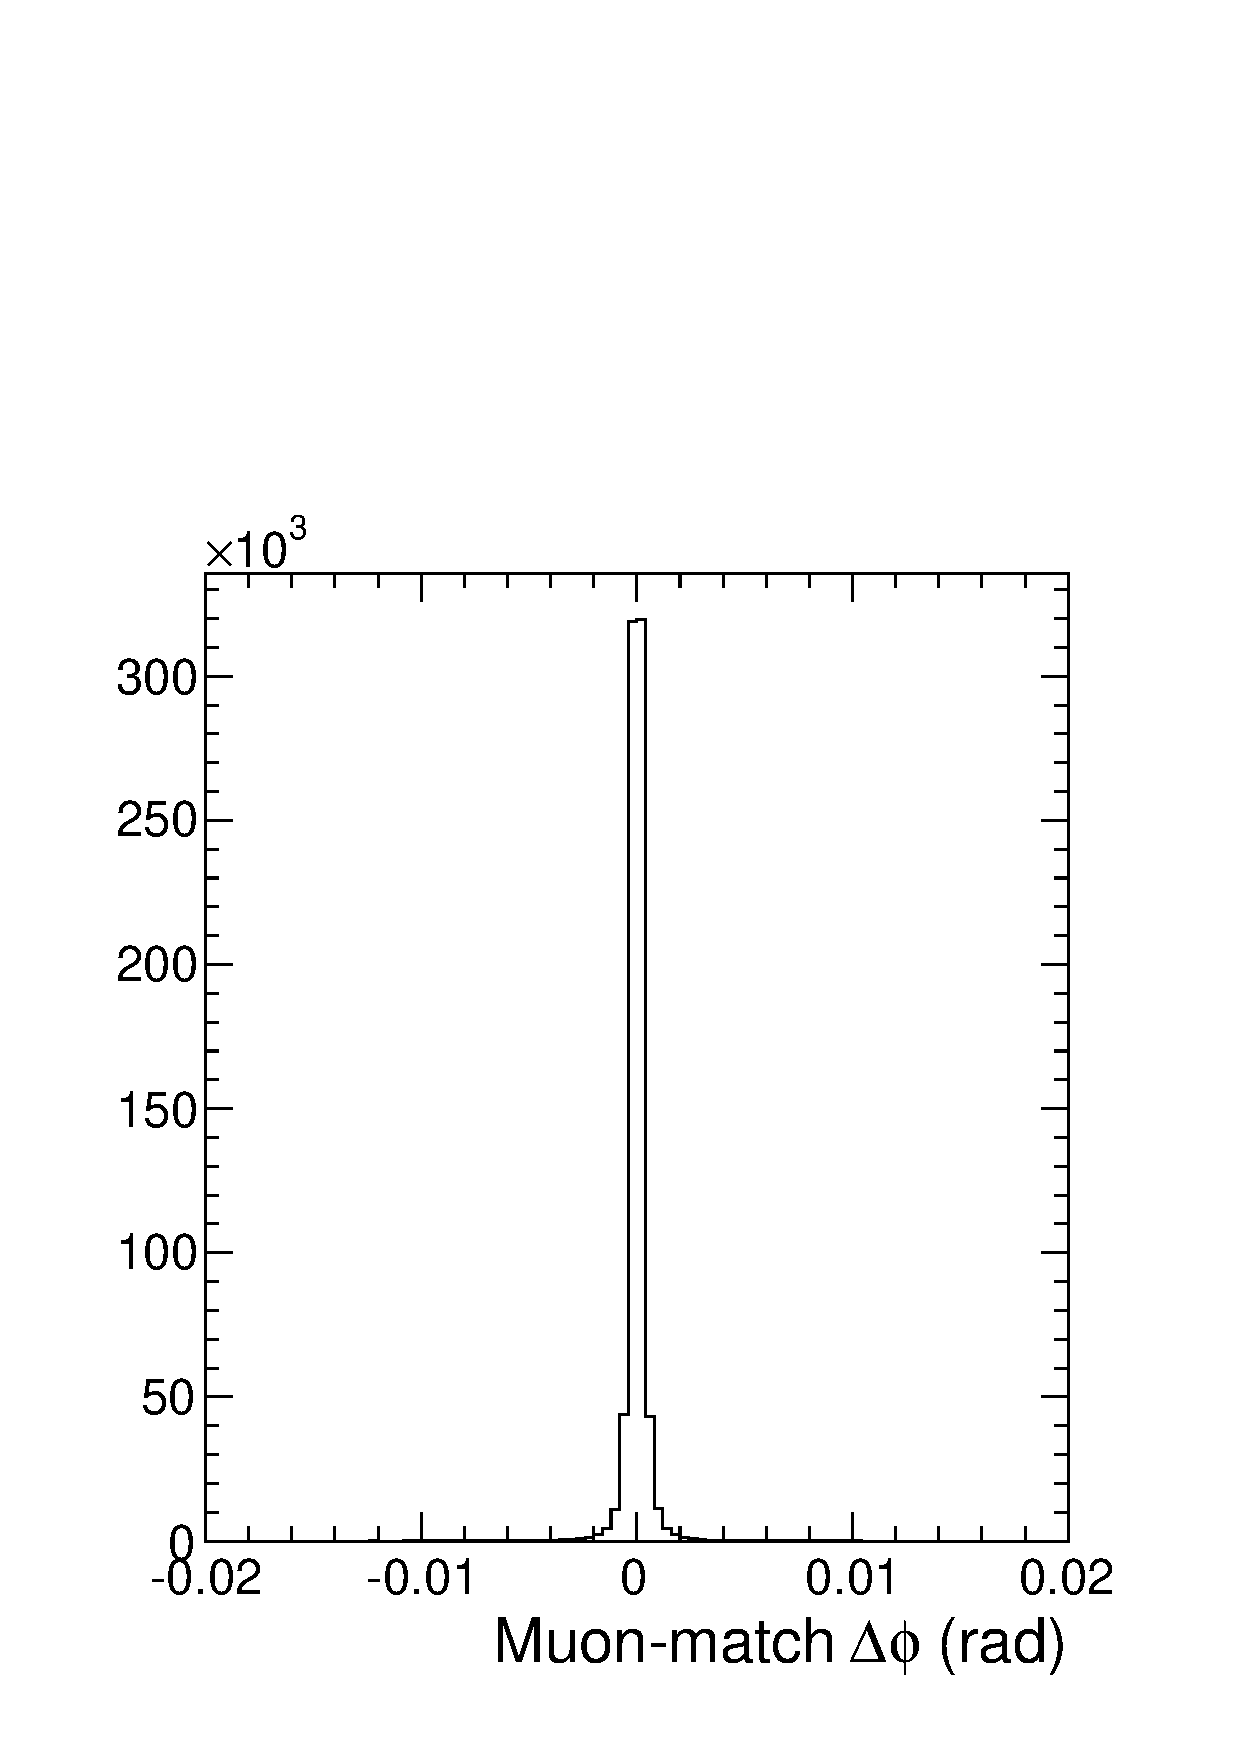
\includegraphics[width=\linewidth]{match_dphi.pdf}
\column{0.5\linewidth}
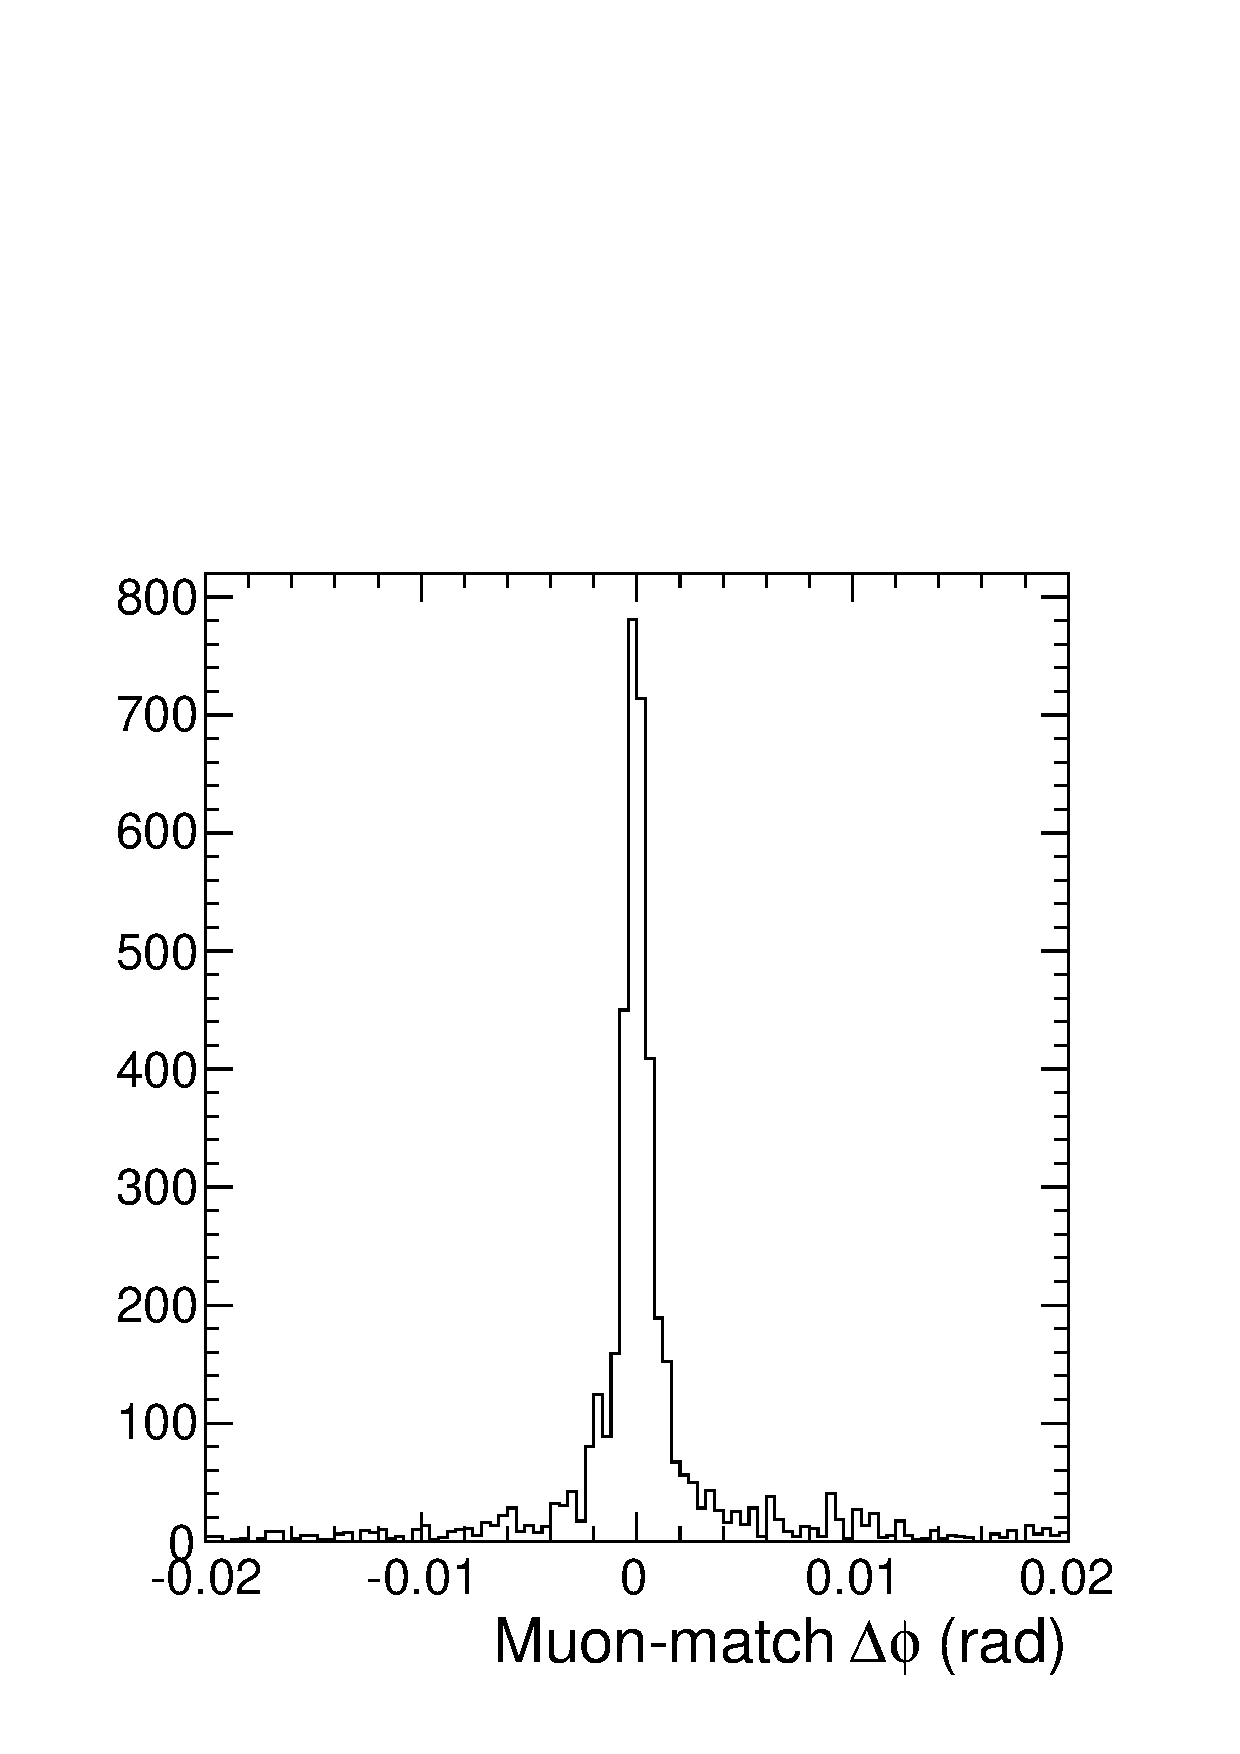
\includegraphics[width=\linewidth]{match_dphi_background.pdf}
\end{columns}
\end{frame}

\begin{frame}
\frametitle{Matched muon $\Delta \eta$}

\begin{itemize}
\item Yes indeed\ldots
\end{itemize}

\begin{columns}
\column{0.5\linewidth}
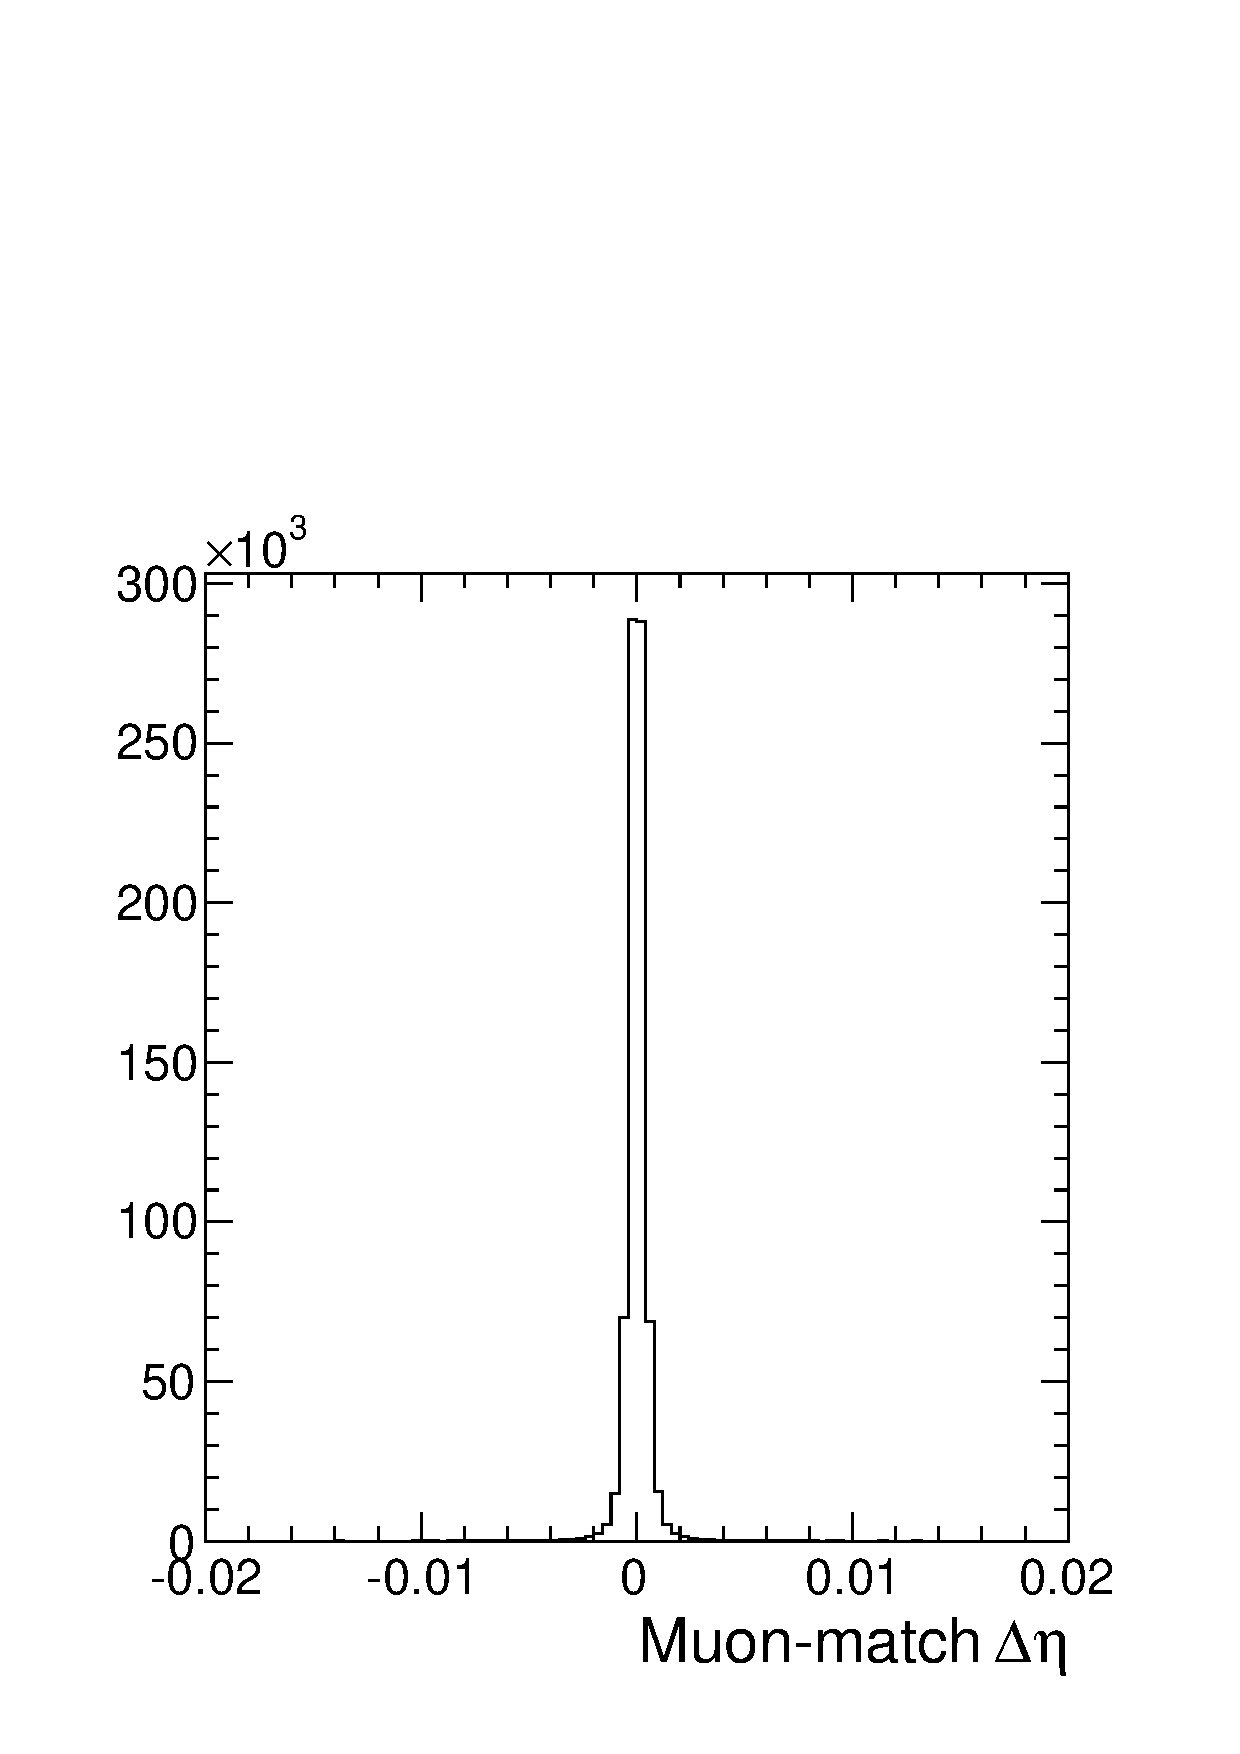
\includegraphics[width=\linewidth]{match_deta.pdf}
\column{0.5\linewidth}
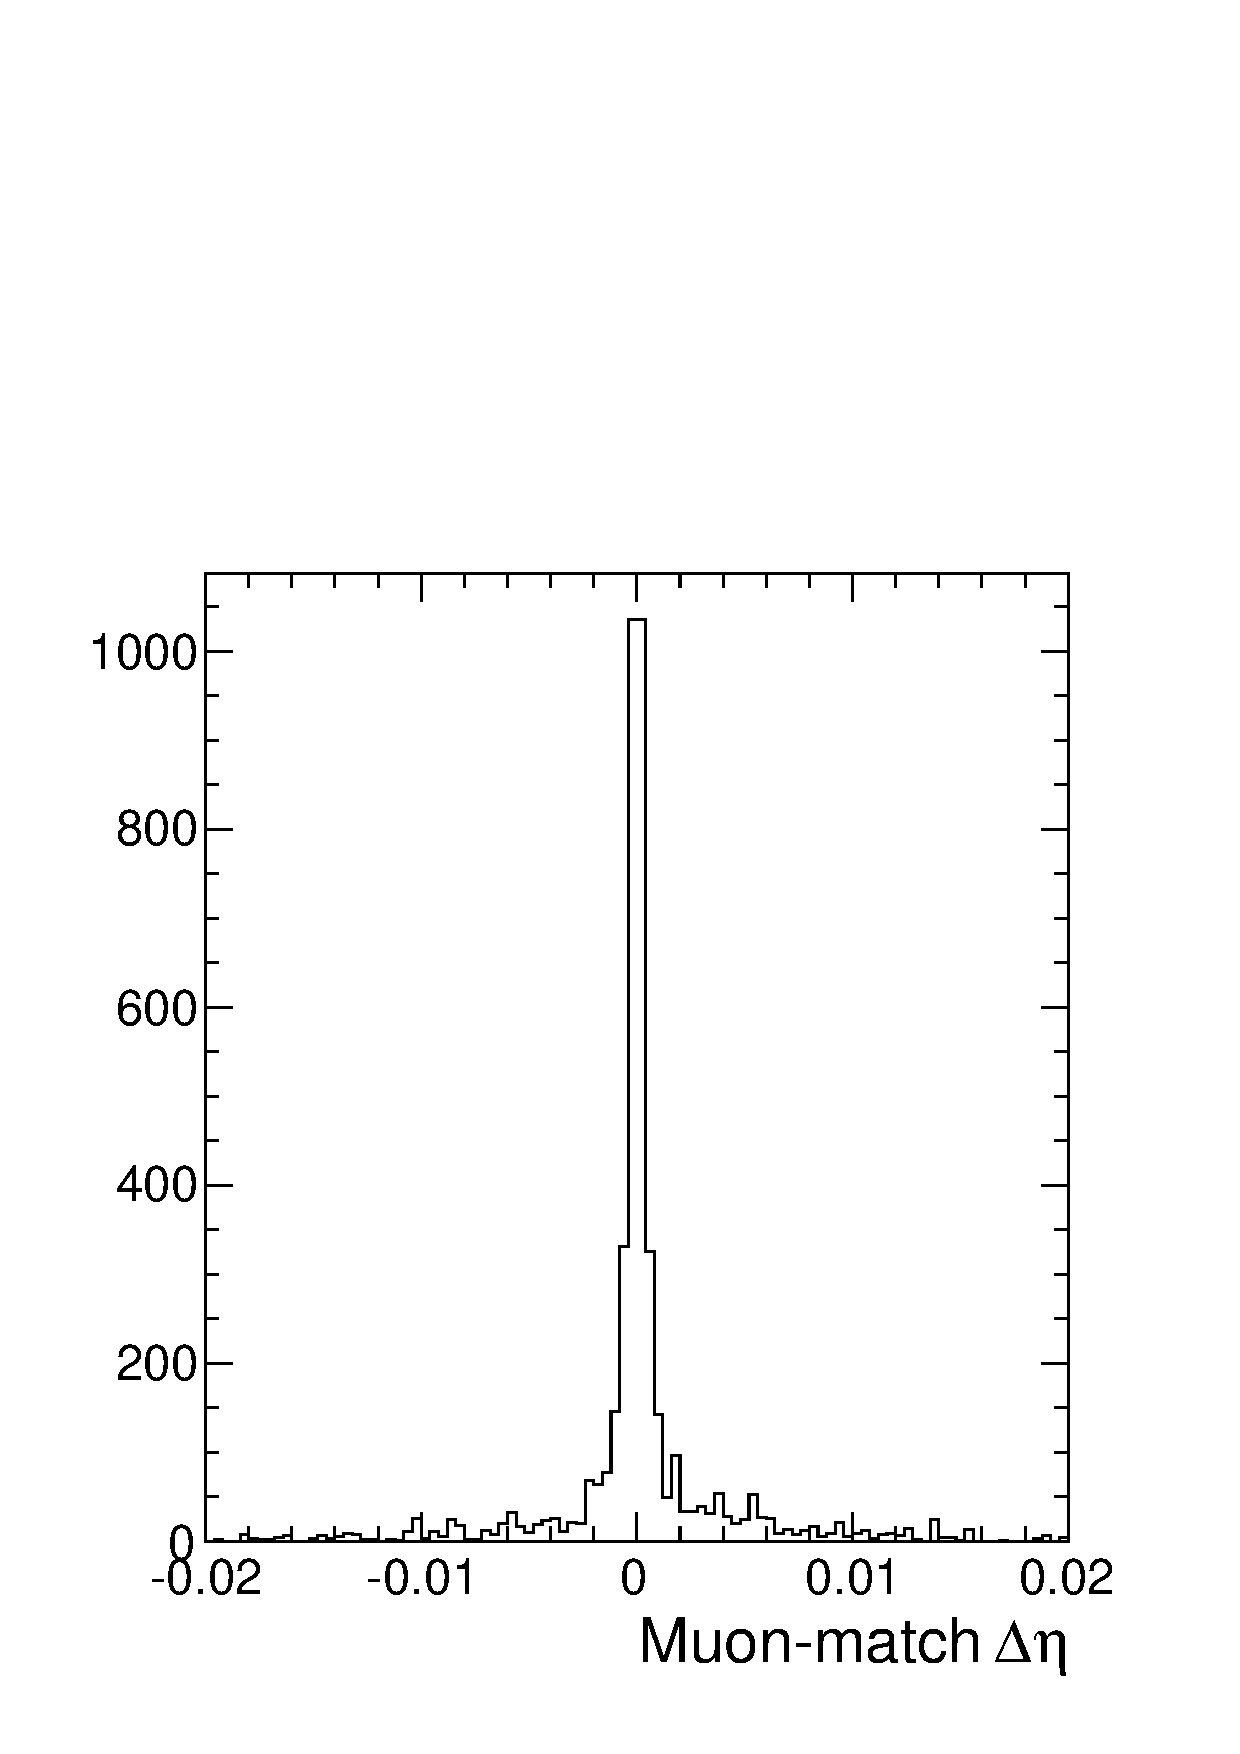
\includegraphics[width=\linewidth]{match_deta_background.pdf}
\end{columns}
\end{frame}

\begin{frame}
\frametitle{Matched muon $\Delta q/p_{T}$}

\begin{itemize}
\item $q/p_{T}$ is curvature, the momentum scale that tracking
  actually measures (as opposed to $p_{T}$, $|vec{p}|$ or something)
\end{itemize}

\begin{columns}
\column{0.5\linewidth}
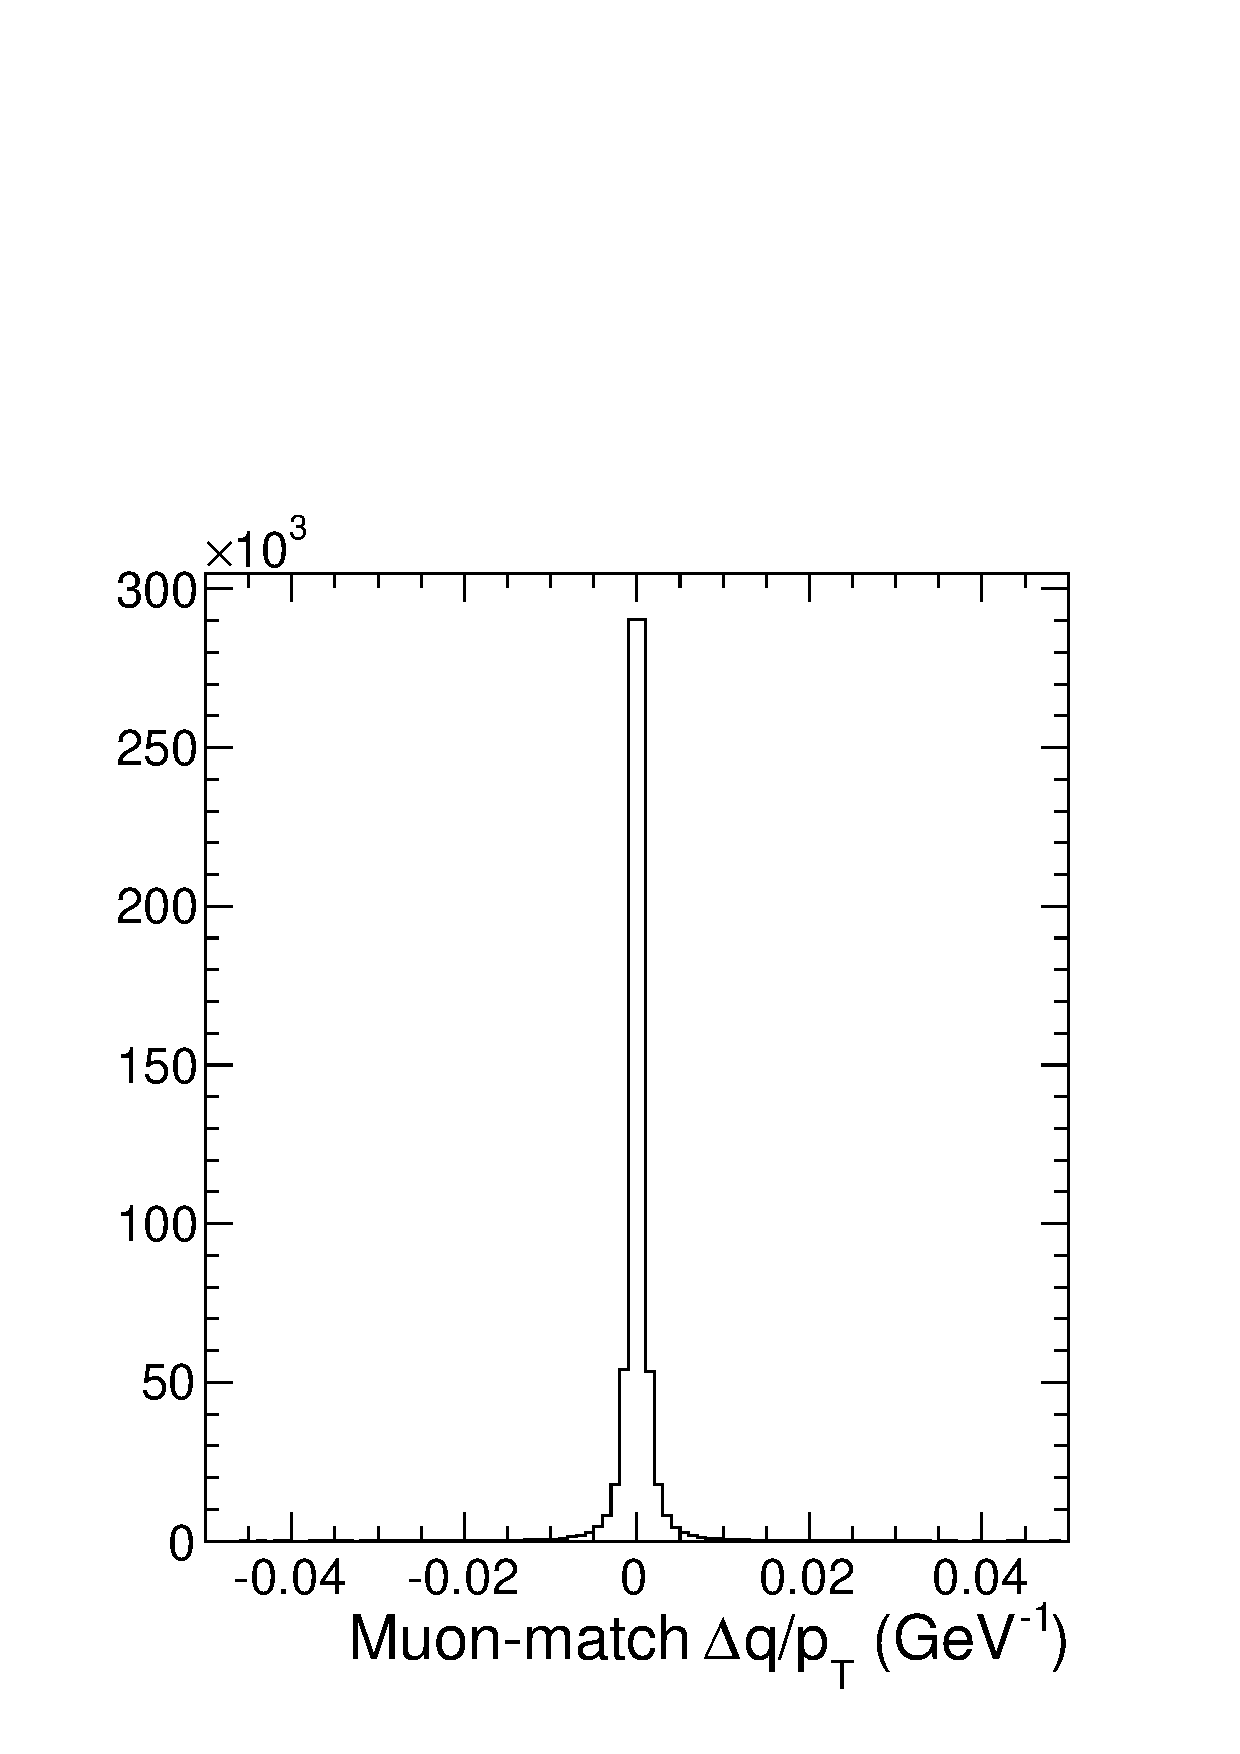
\includegraphics[width=\linewidth]{match_dqoverpt.pdf}
\column{0.5\linewidth}
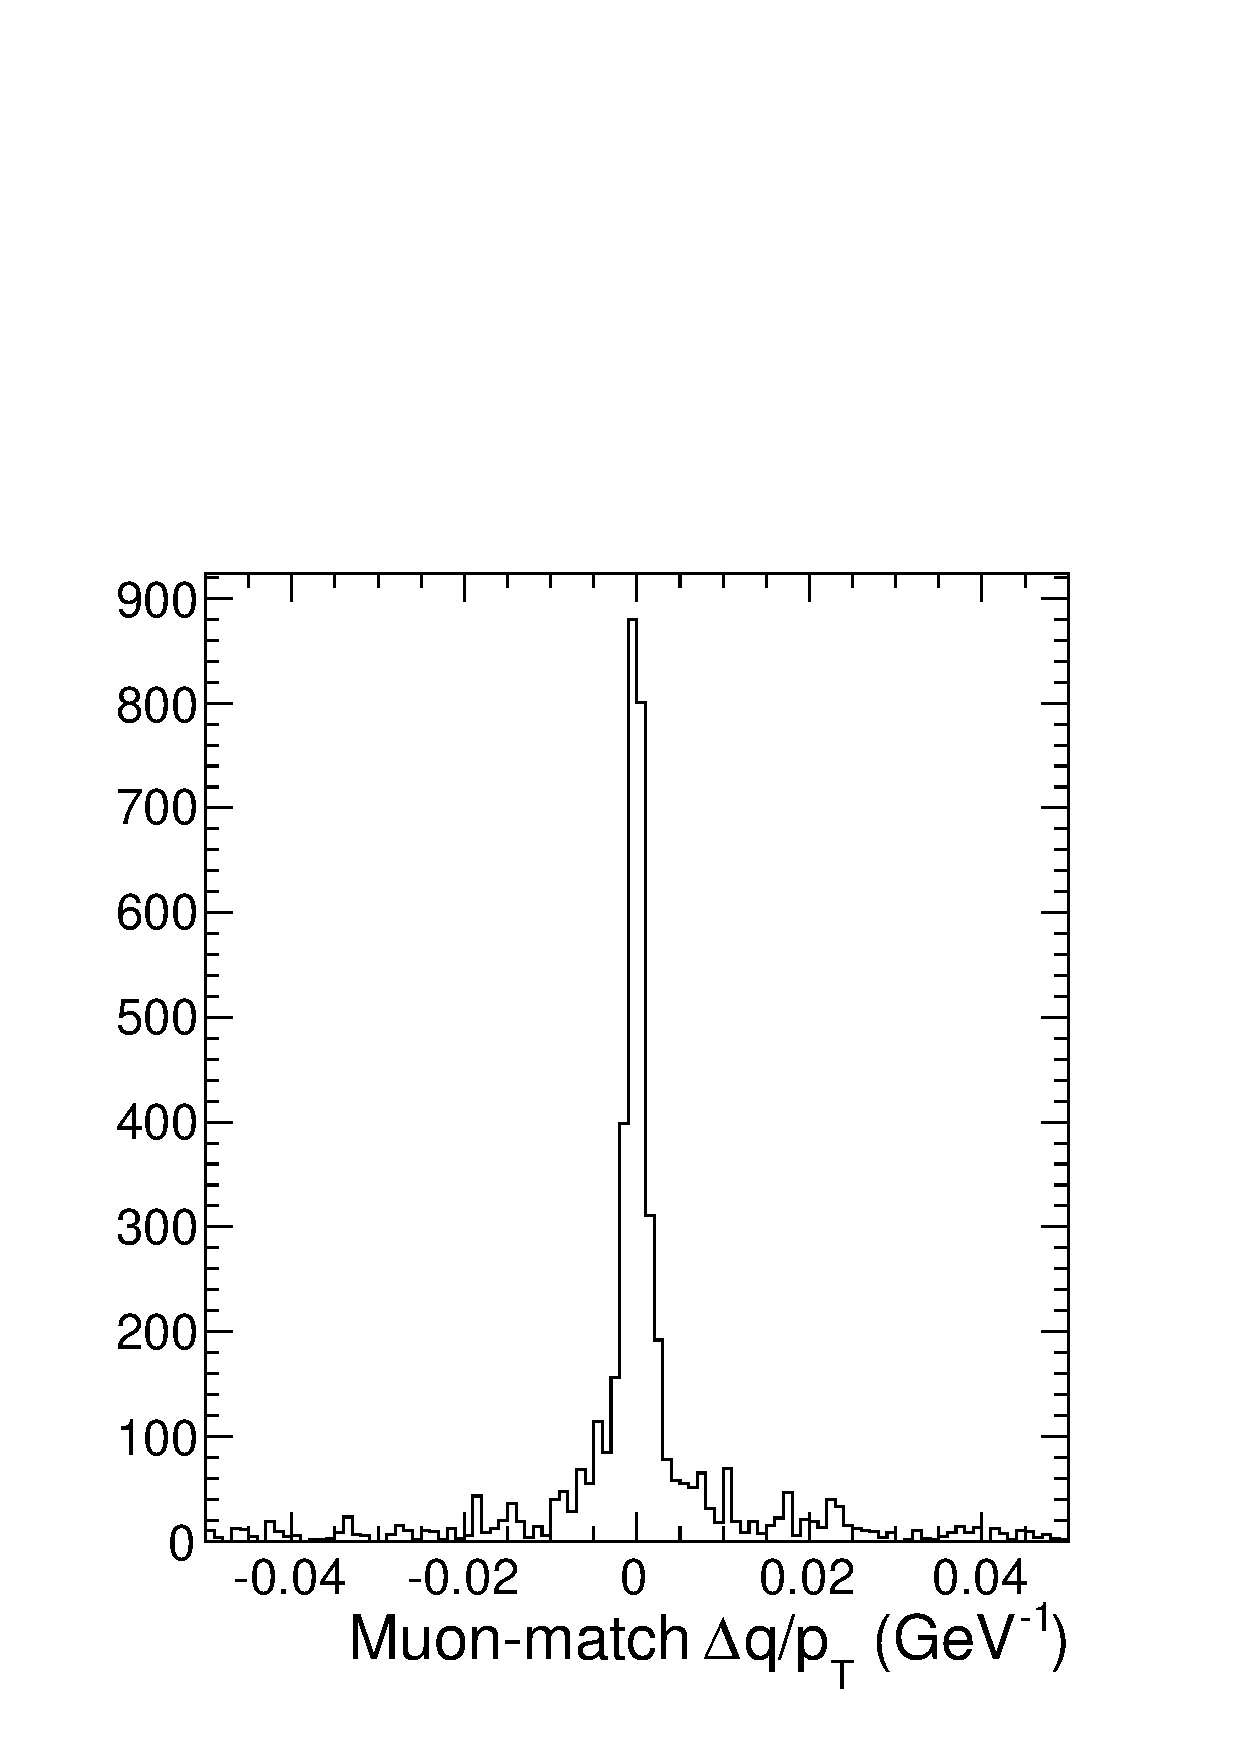
\includegraphics[width=\linewidth]{match_dqoverpt_background.pdf}
\end{columns}
\end{frame}

\begin{frame}
\frametitle{ECAL isolation variable}

\begin{itemize}
\item PAT also gives us $\sum p_T$ around each muon ($R < 0.3$) for free
\item Don't take these plots as definitive: when applied to muon pairs, they include double-counting
\item Muons contribute negligibly to calorimeter energy (minimum-ionizing)
\end{itemize}

\begin{columns}
\column{0.5\linewidth}
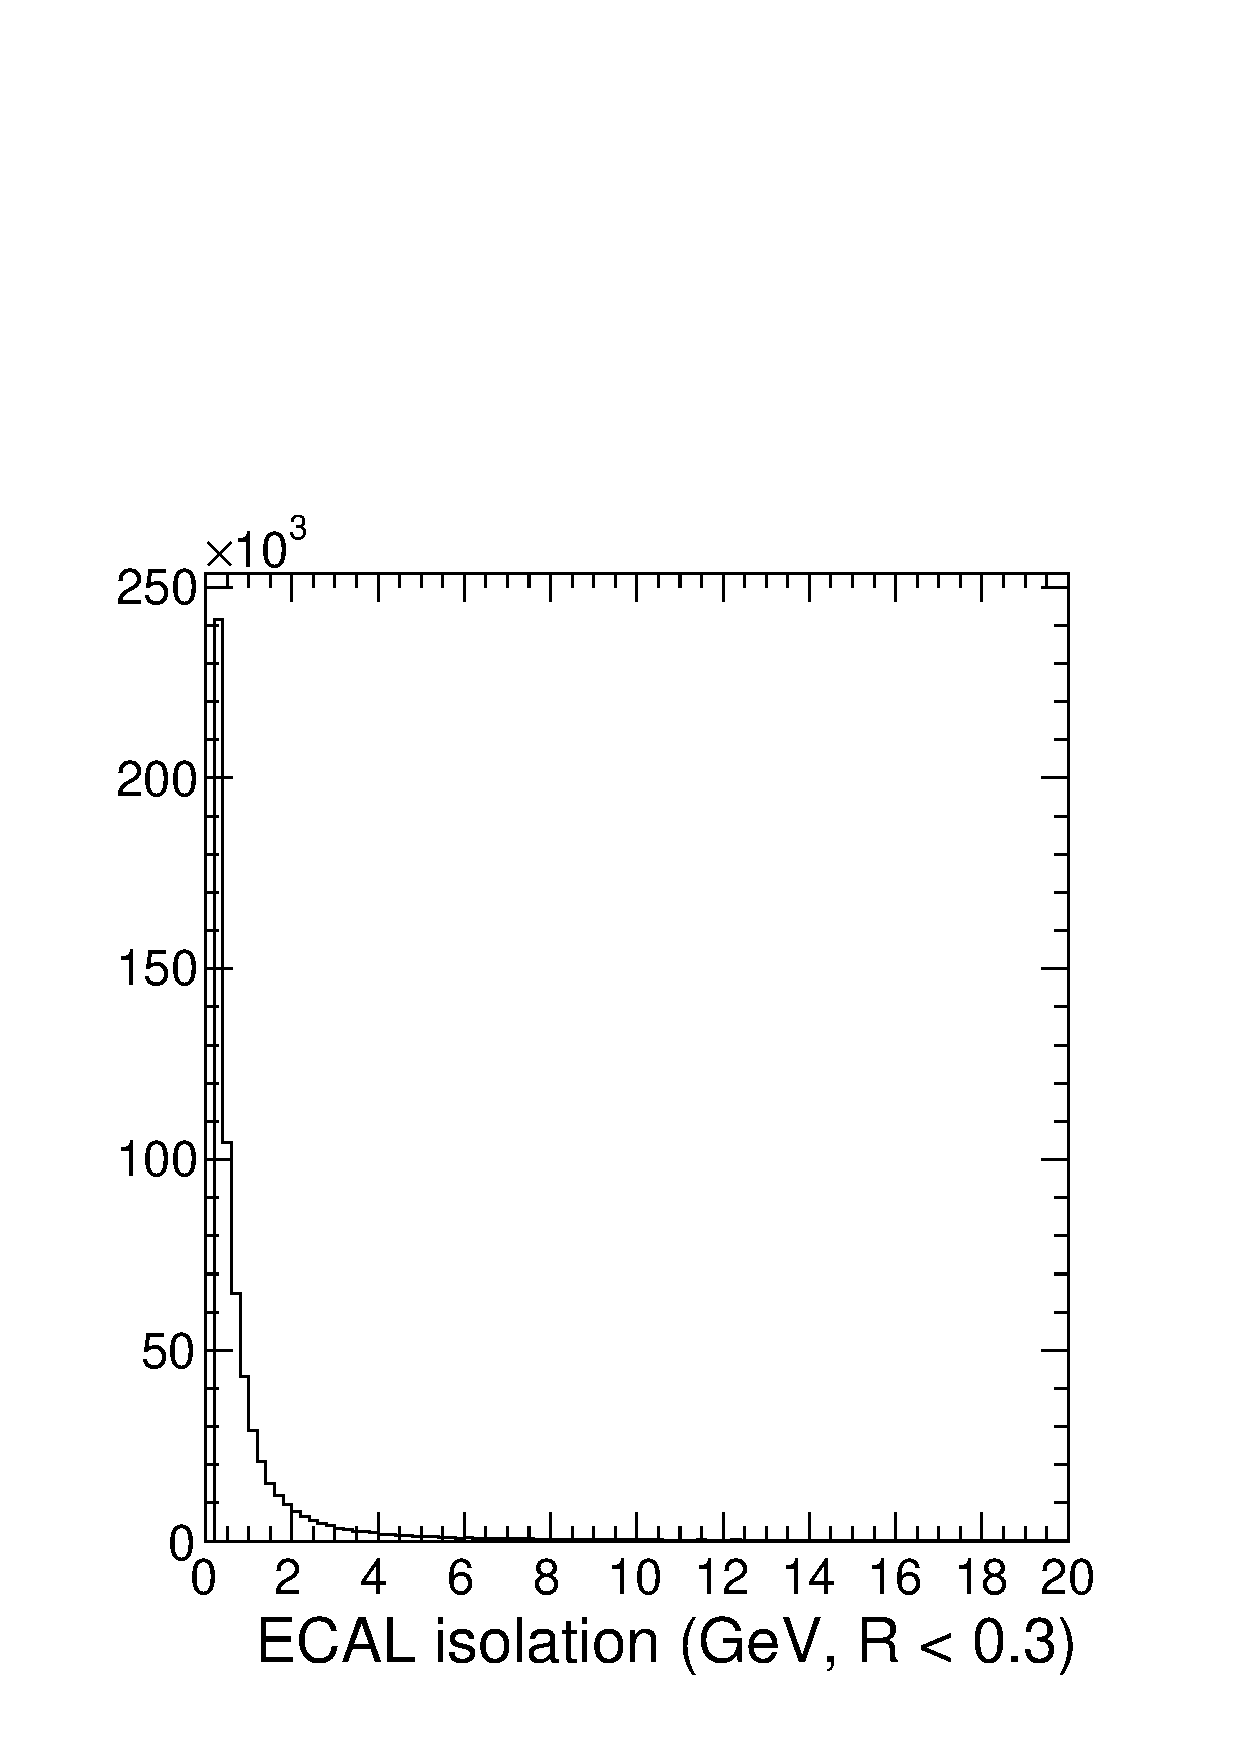
\includegraphics[width=\linewidth]{ecaliso.pdf}
\column{0.5\linewidth}
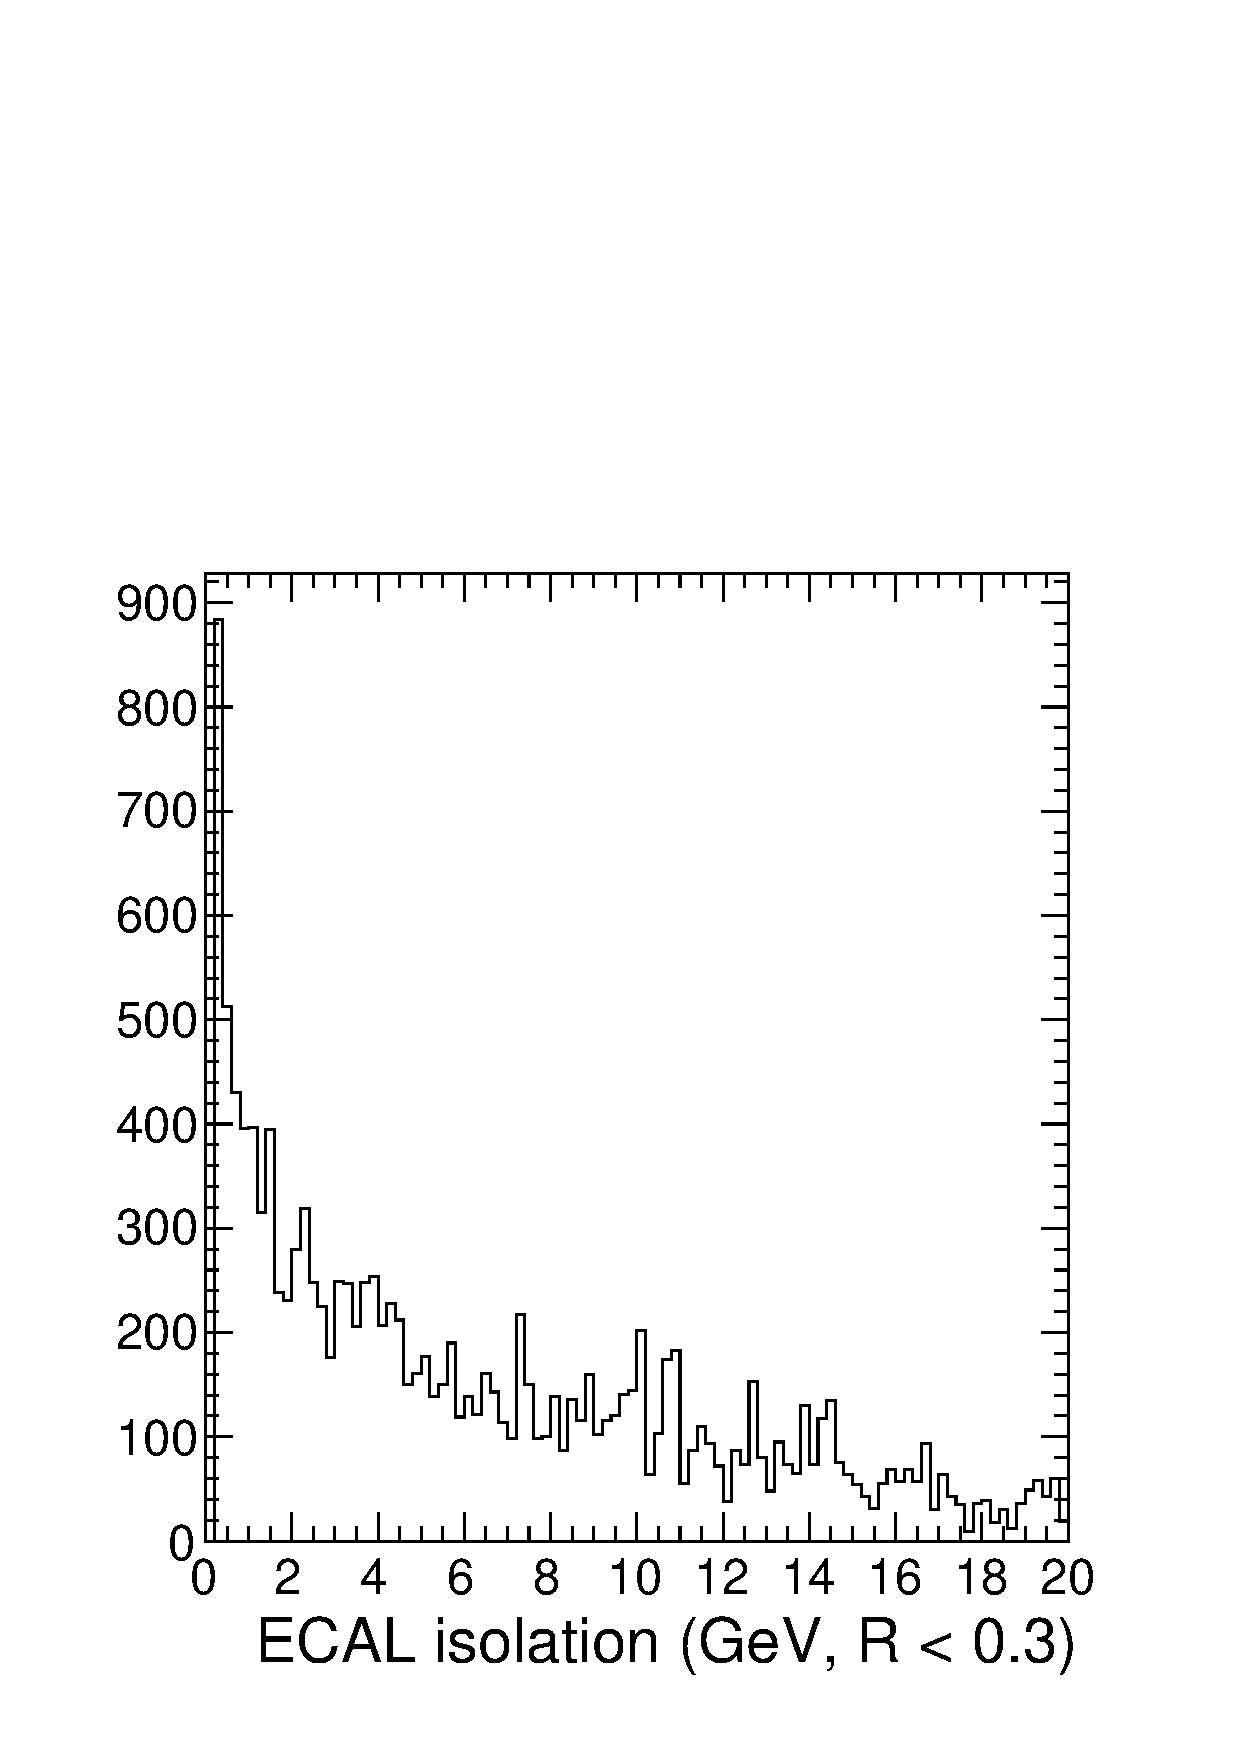
\includegraphics[width=\linewidth]{ecaliso_background.pdf}
\end{columns}
\end{frame}

\begin{frame}
\frametitle{HCAL isolation variable}

\begin{itemize}
\item Same thing for HCAL\ldots
\end{itemize}

\begin{columns}
\column{0.5\linewidth}
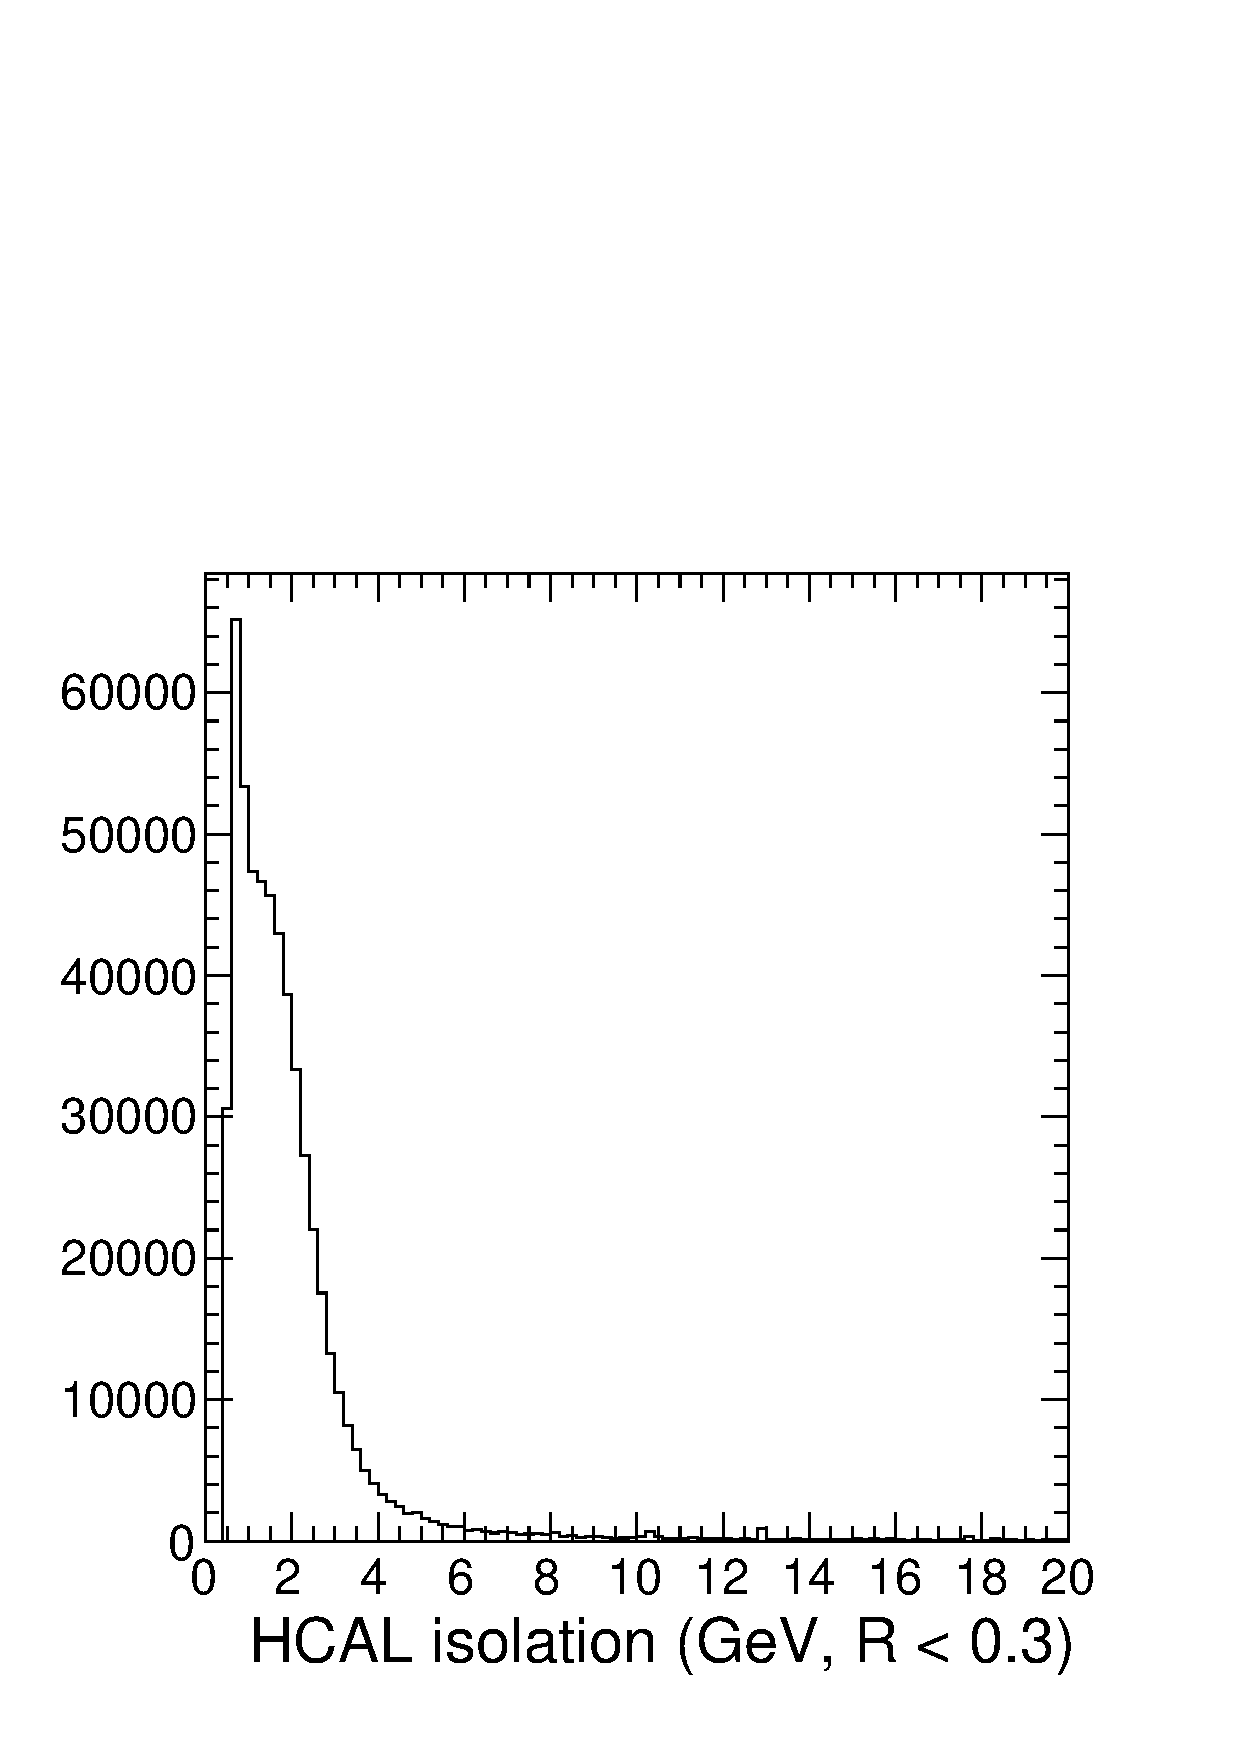
\includegraphics[width=\linewidth]{hcaliso.pdf}
\column{0.5\linewidth}
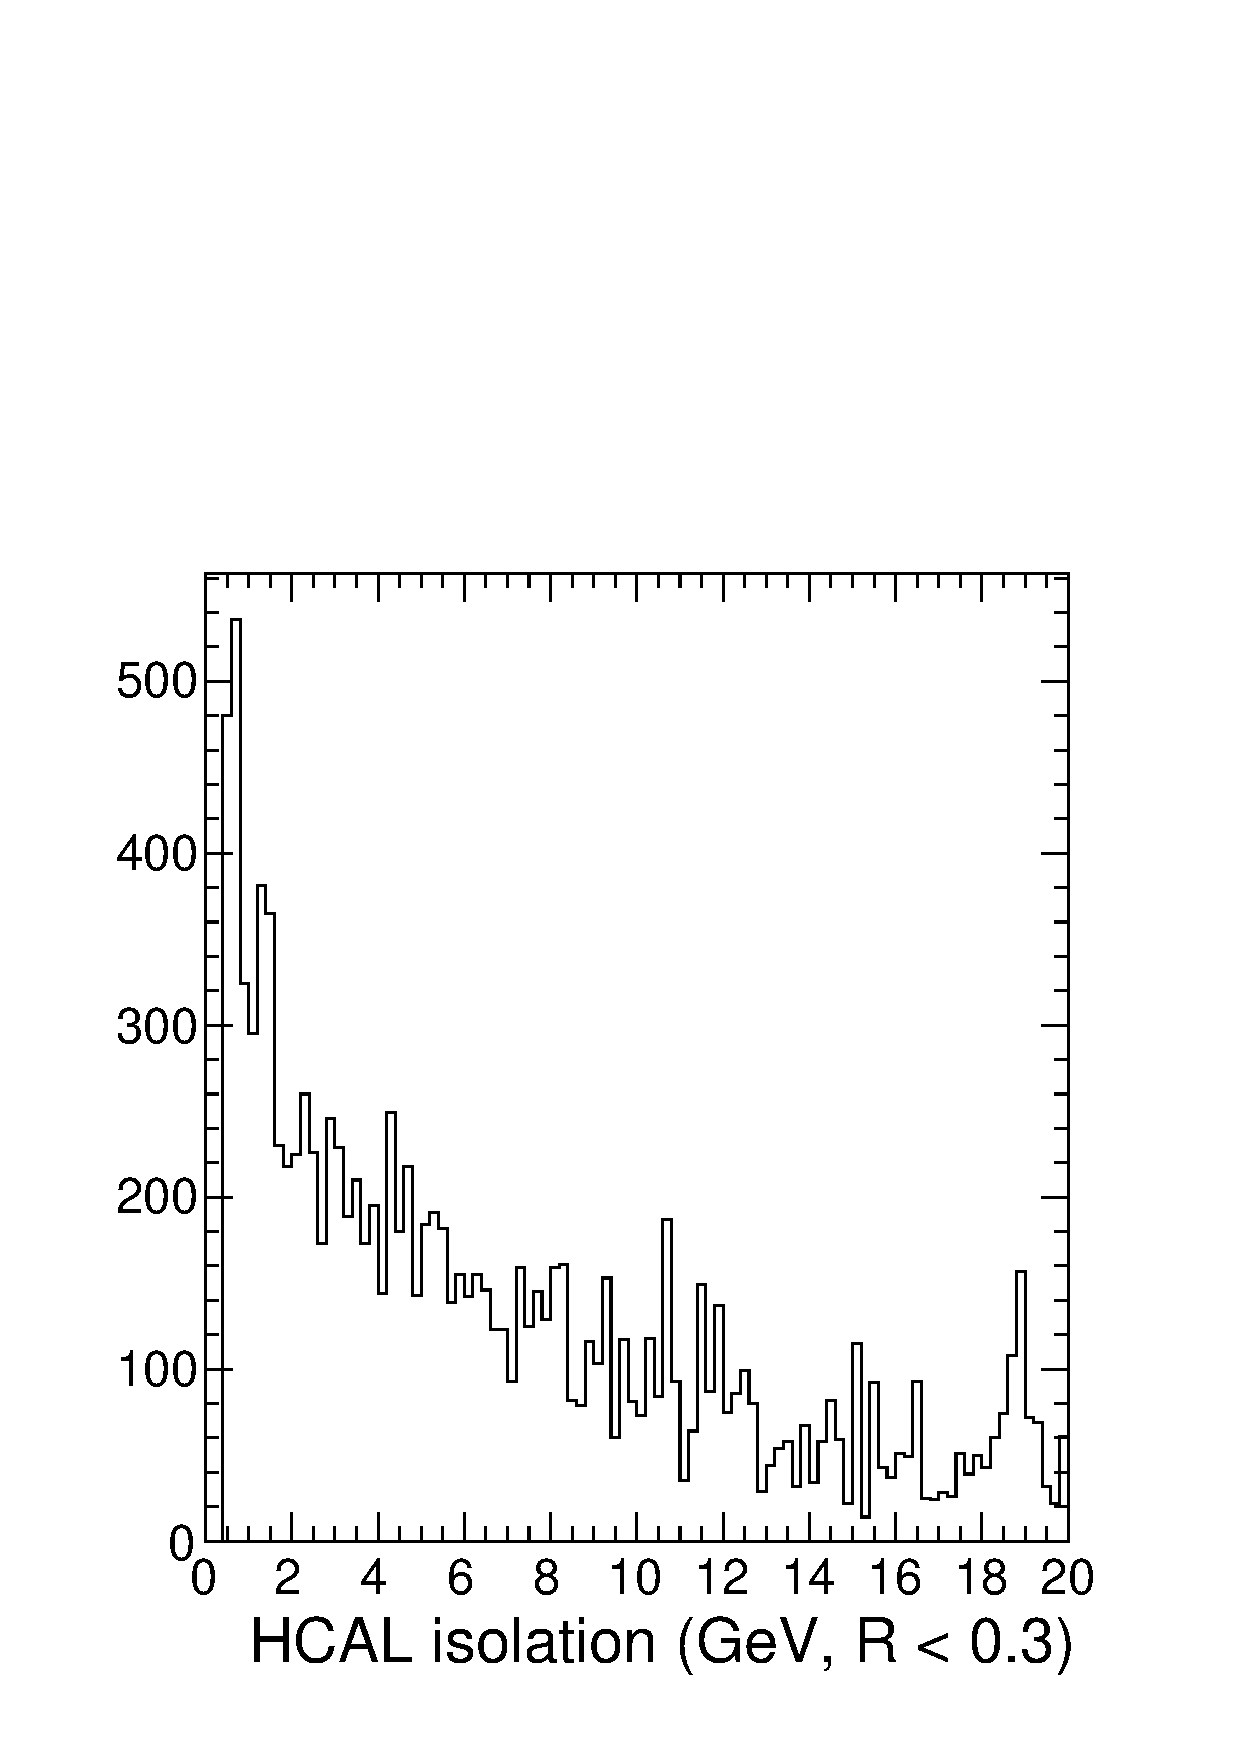
\includegraphics[width=\linewidth]{hcaliso_background.pdf}
\end{columns}
\end{frame}

\begin{frame}
\frametitle{``Track isolation'' variable}

\begin{itemize}
\item PAT's ``track isolation'' is not what we want, because the
  second muon in each pair often appears in the other's isolation
  cone
\item This is what our isolation definition improves
\end{itemize}

\begin{columns}
\column{0.5\linewidth}
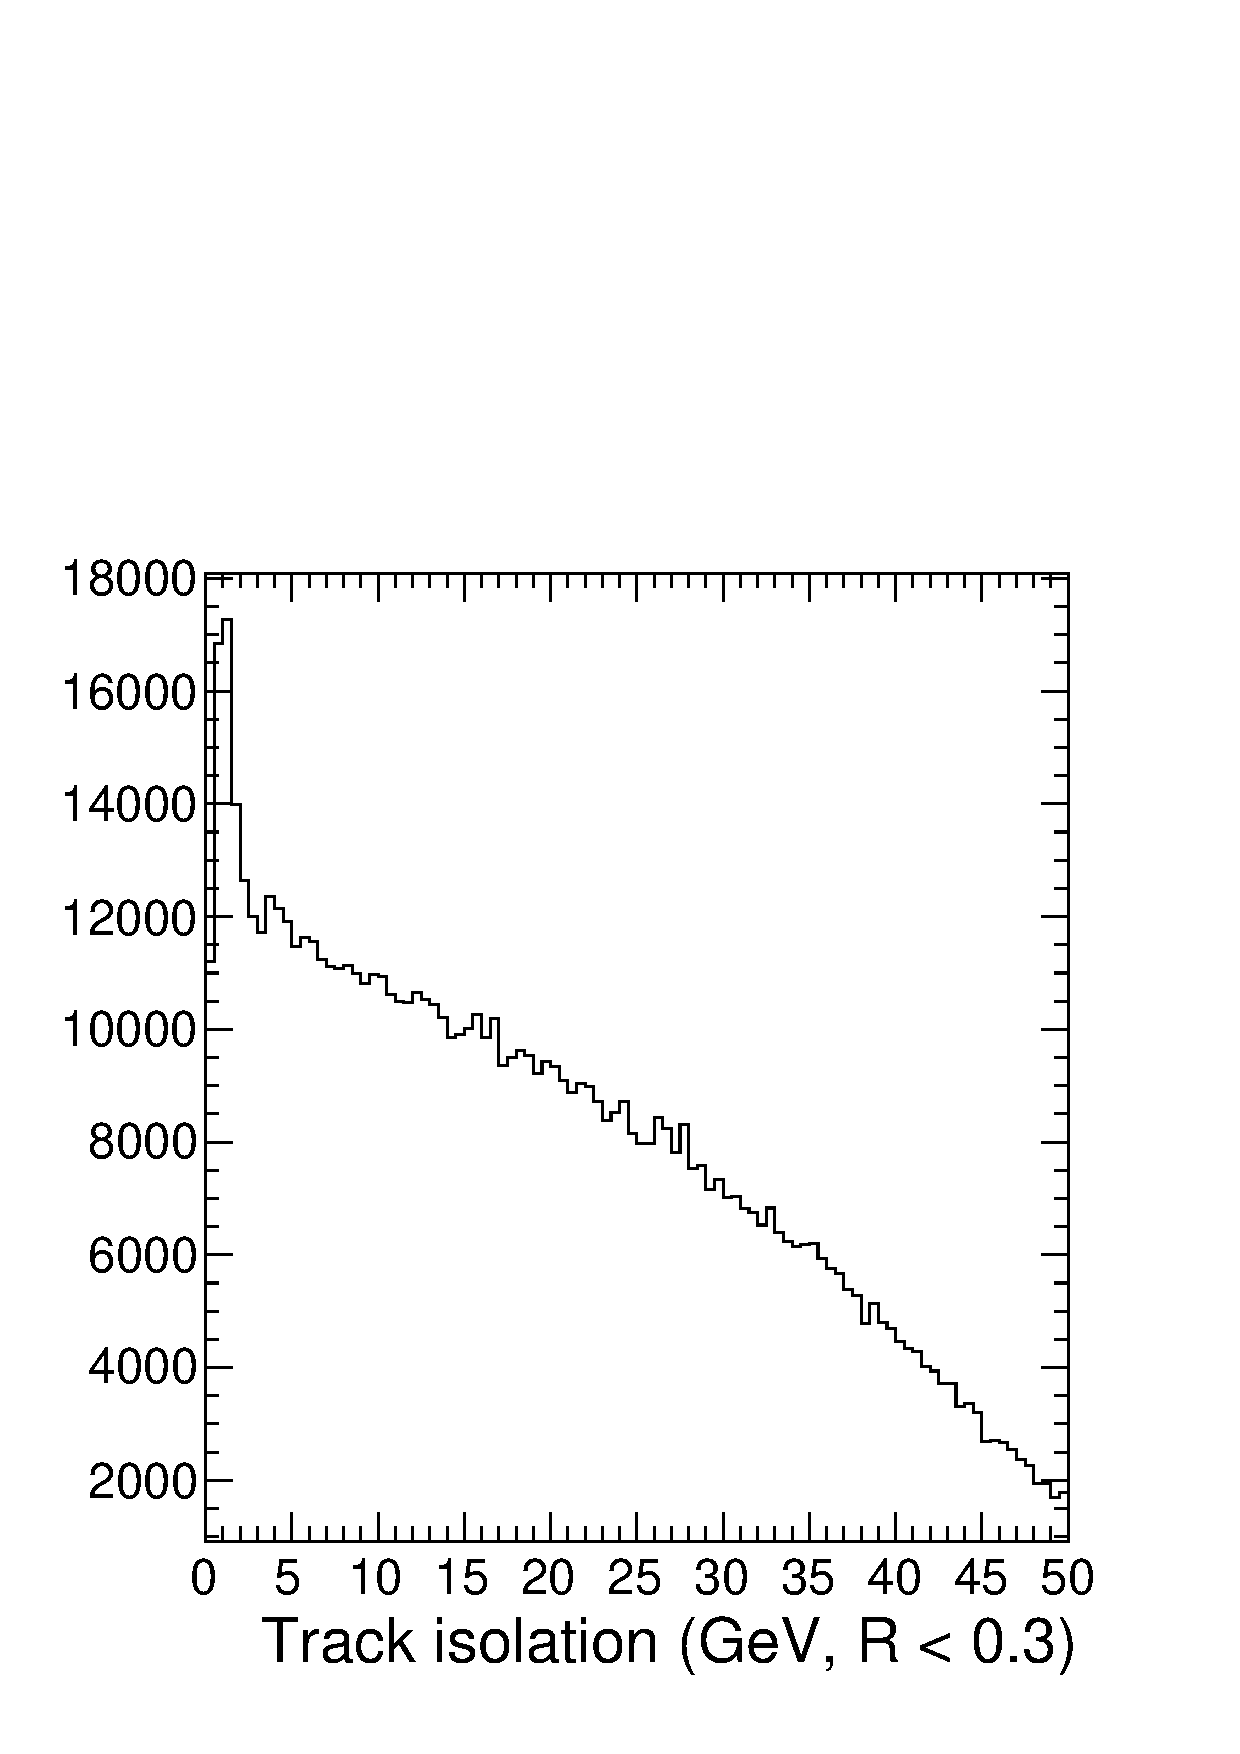
\includegraphics[width=\linewidth]{trackiso.pdf}
\column{0.5\linewidth}
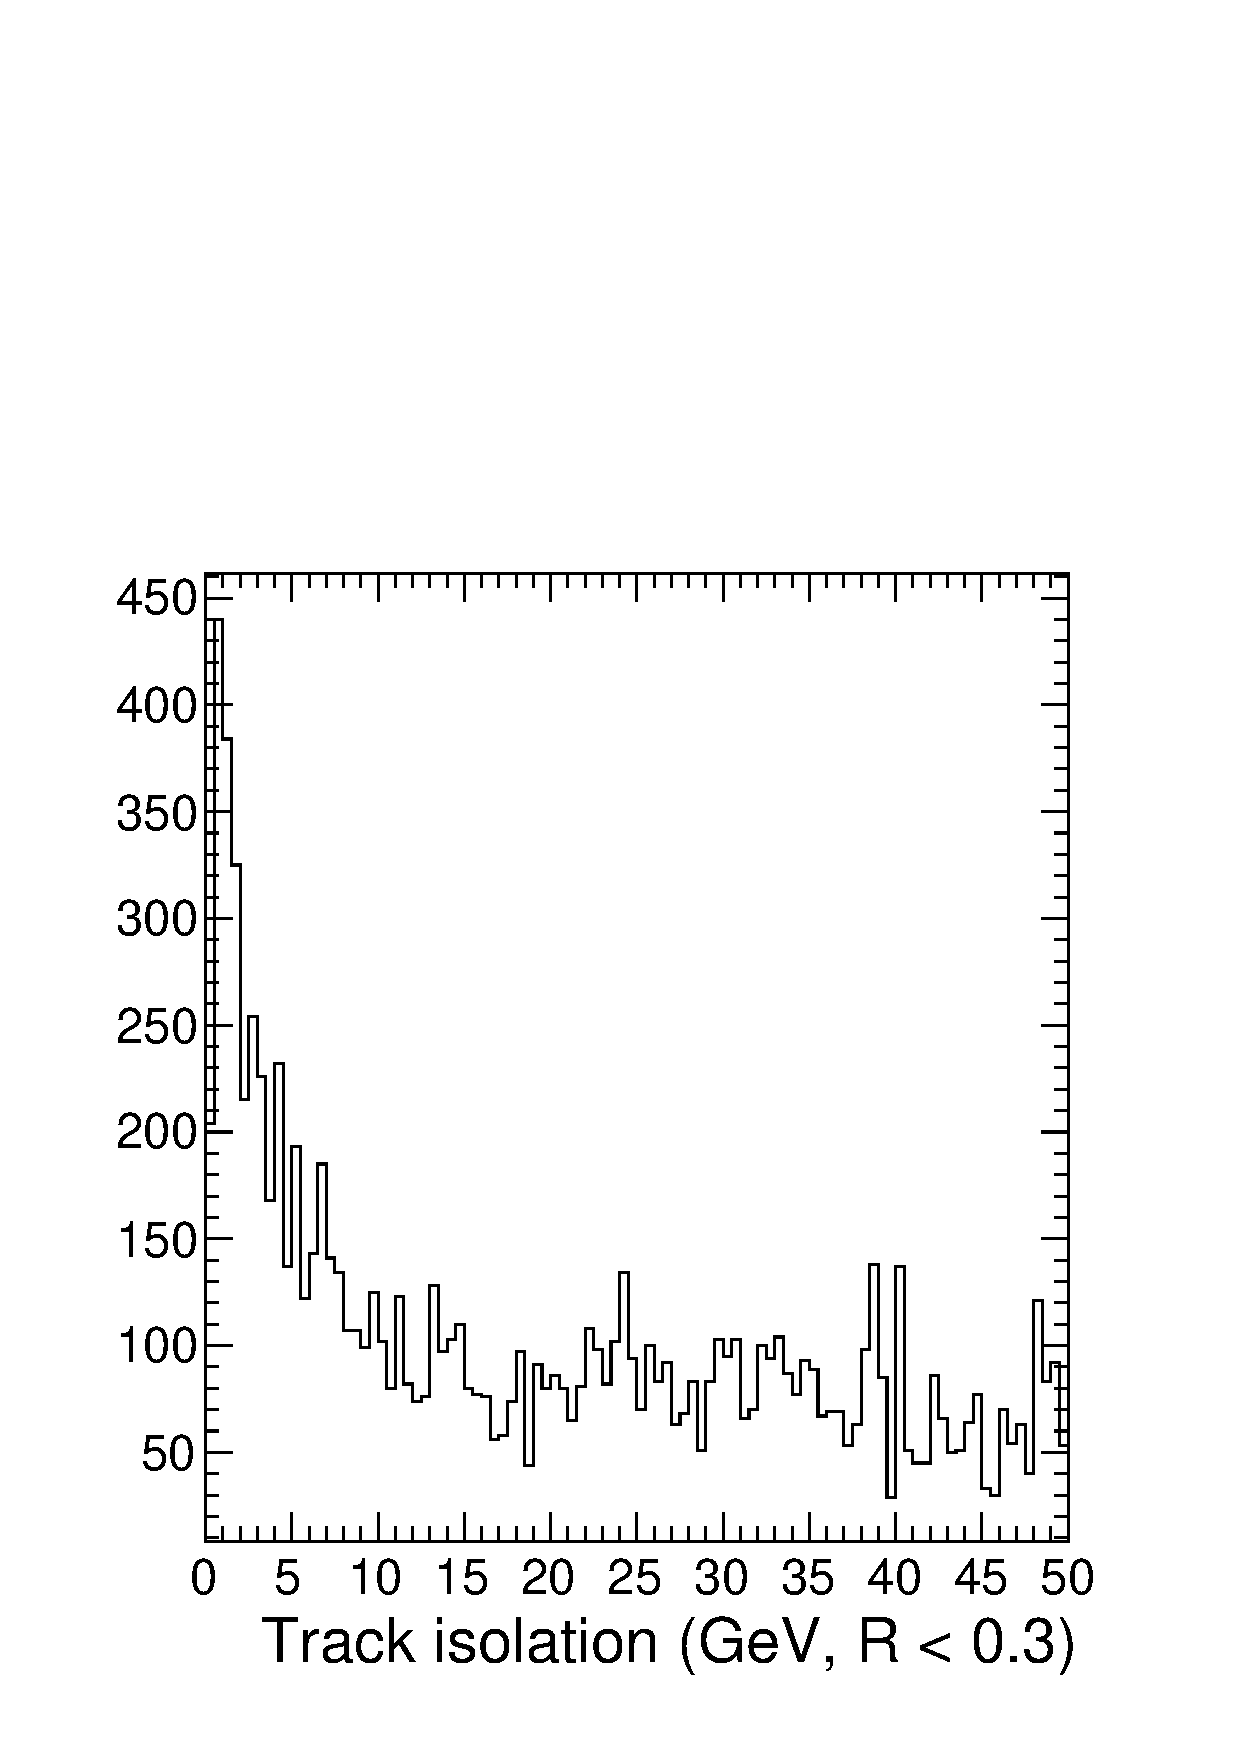
\includegraphics[width=\linewidth]{trackiso_background.pdf}
\end{columns}
\end{frame}

\begin{frame}
\frametitle{Good track isolation}

\begin{itemize}
\item Track isolation without counting the muons and without
  double-counting tracks in both muons' cones
\item Aysen has developed an isolation variable like this, but we'd
  have to compare notes to see if it's exactly the same
\end{itemize}

\begin{columns}
\column{0.5\linewidth}
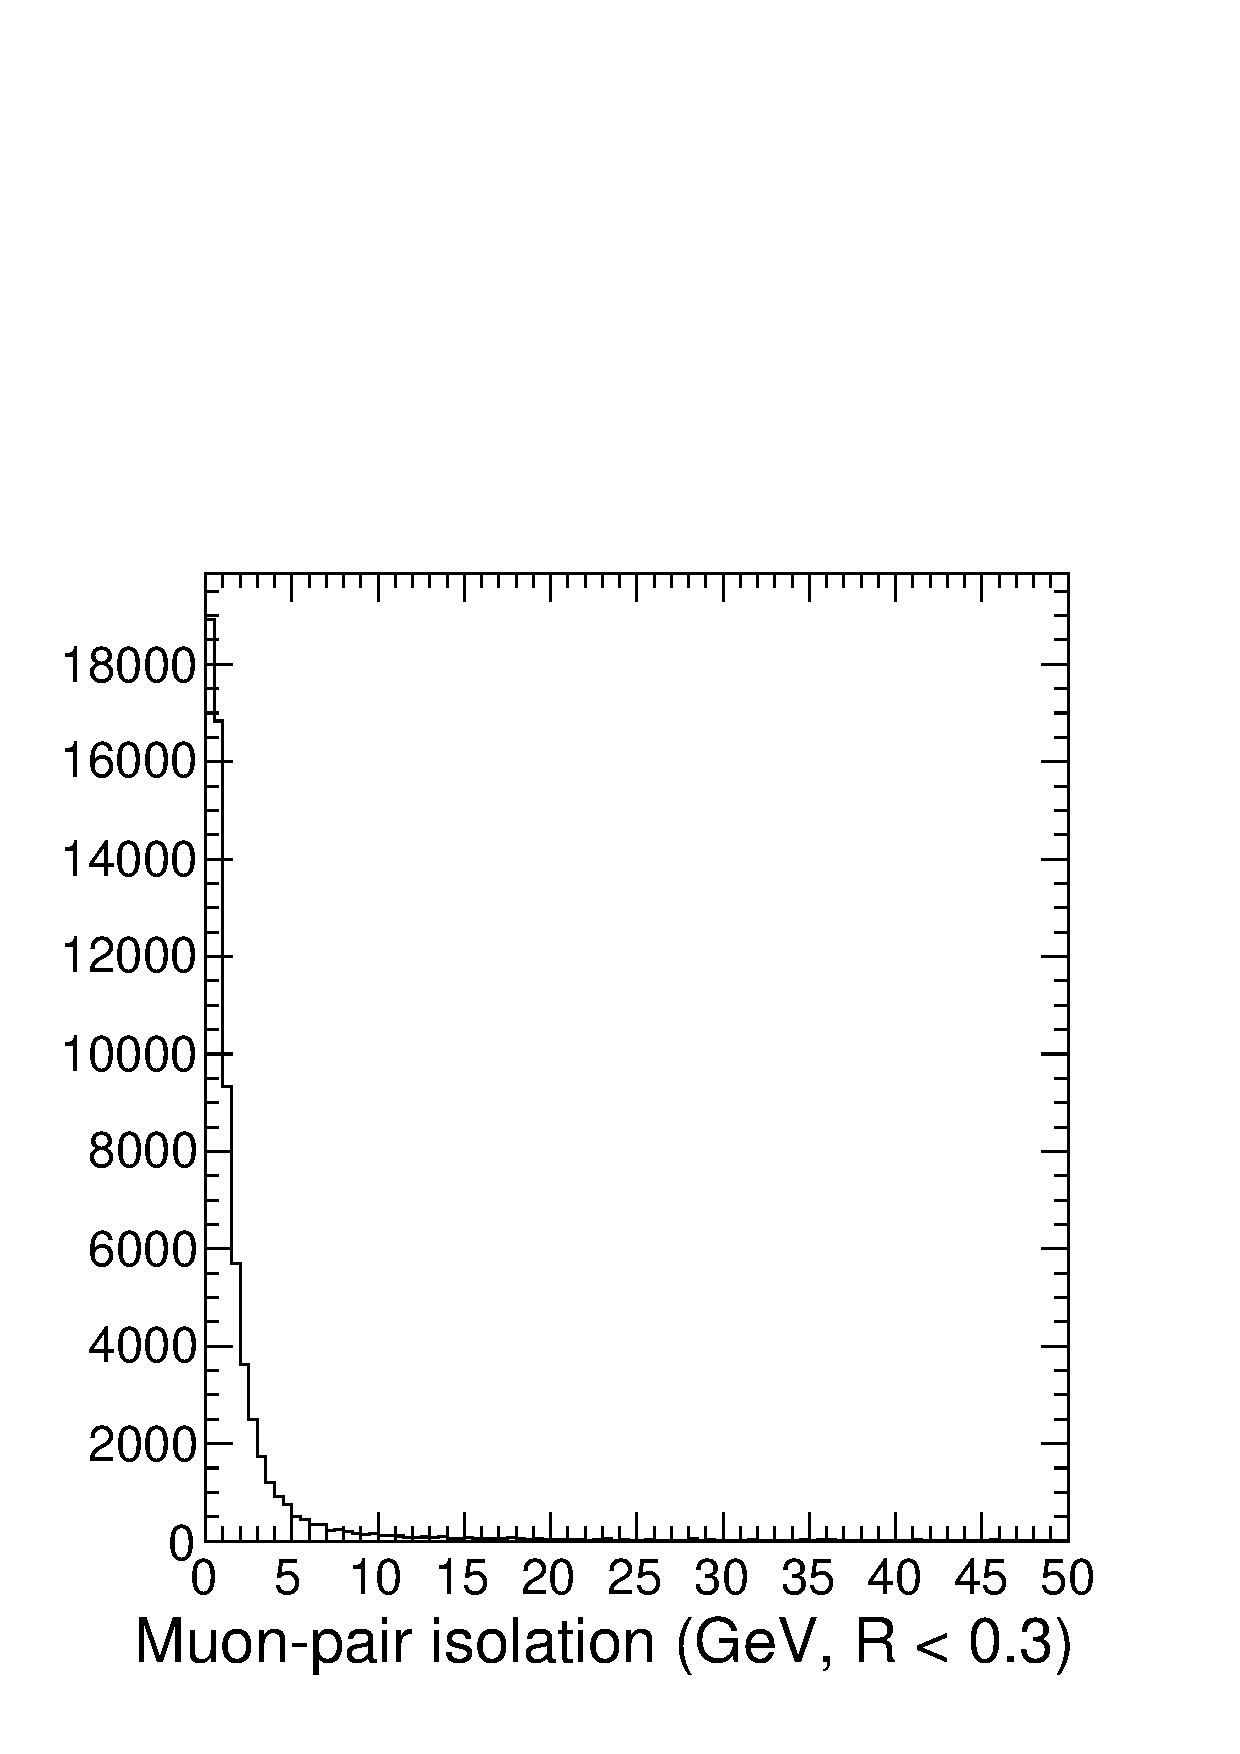
\includegraphics[width=\linewidth]{bubbleiso.pdf}
\column{0.5\linewidth}
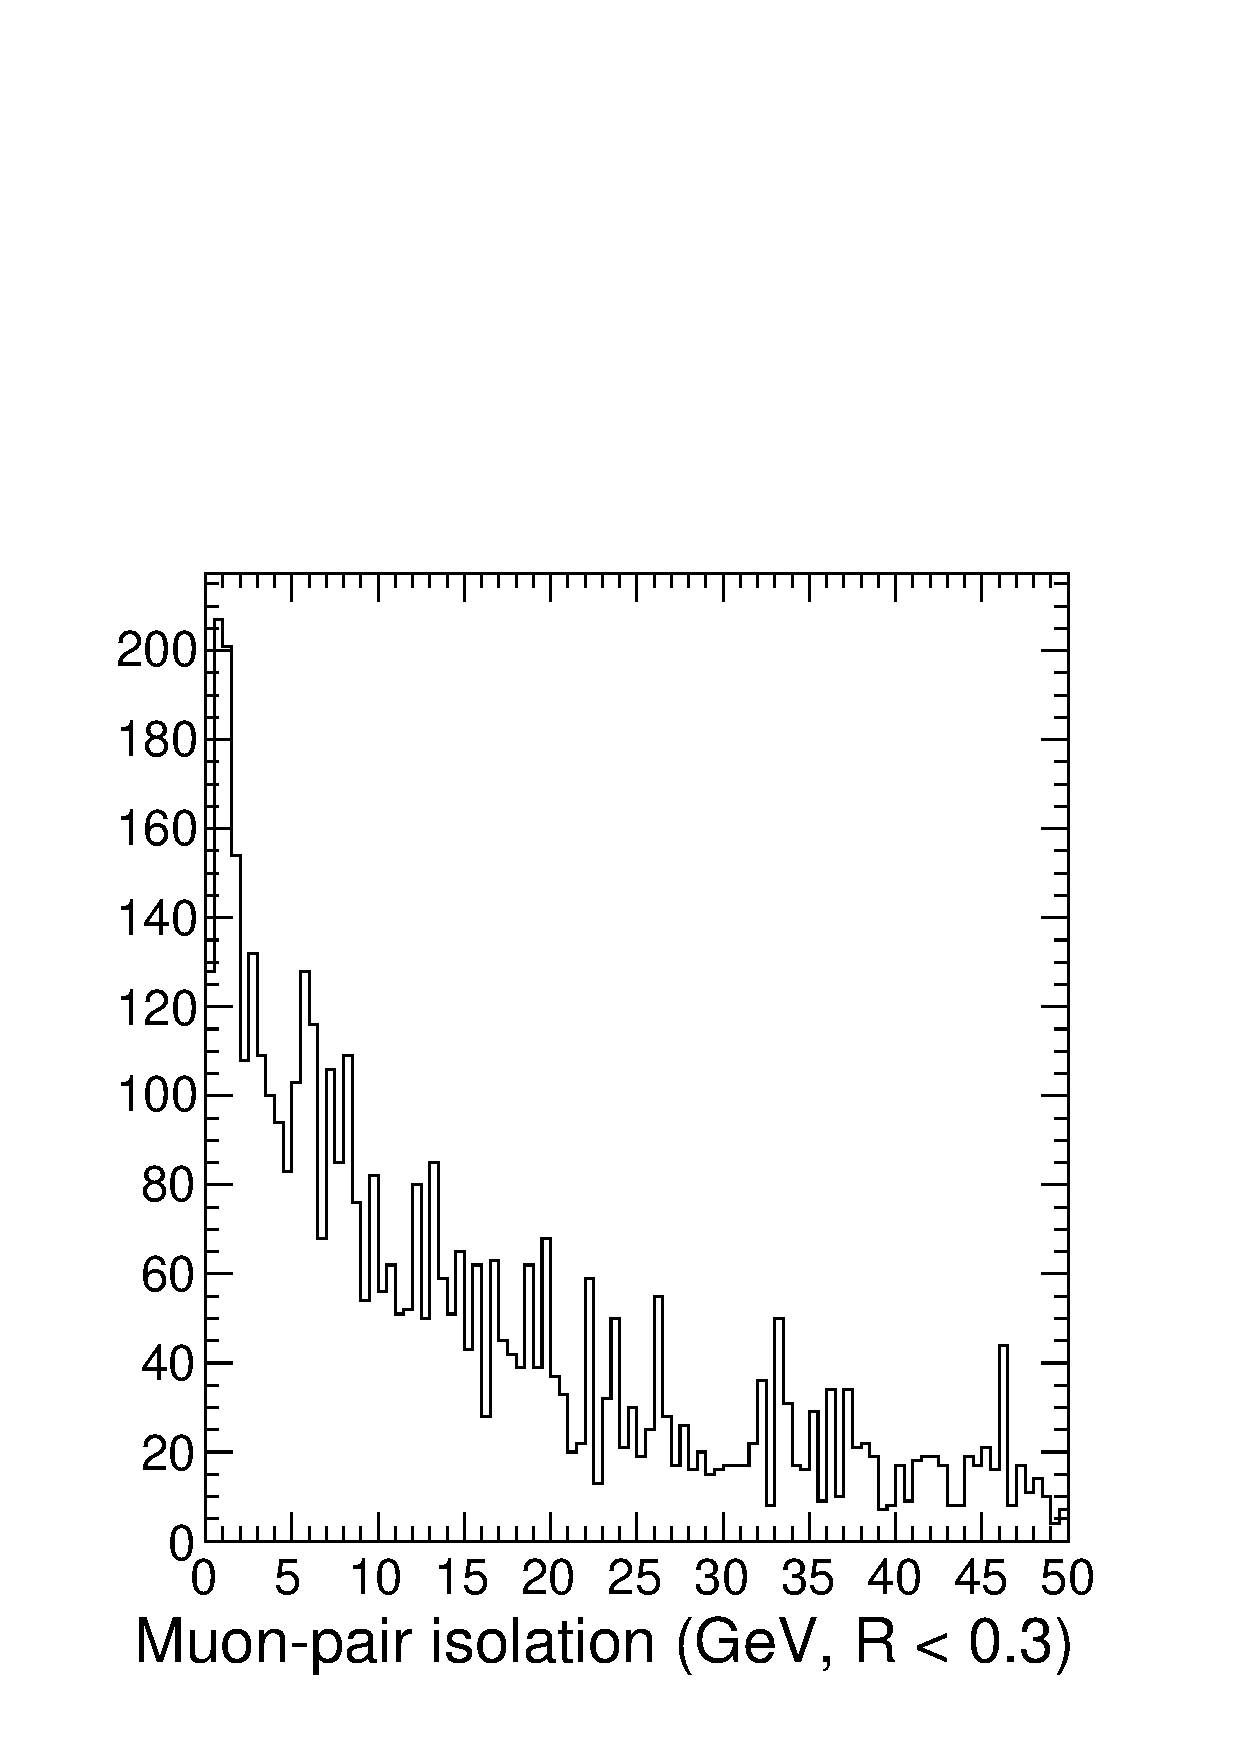
\includegraphics[width=\linewidth]{bubbleiso_background.pdf}
\end{columns}
\end{frame}

\begin{frame}
\frametitle{Good track iso vs.\ calo iso}

\begin{itemize}
\item They're not strongly correlated: can improve isolation by cutting on both
\item Careful with the interpretation: we're still double-counting some calo $\sum p_{T}$
\end{itemize}

\begin{columns}
\column{0.5\linewidth}
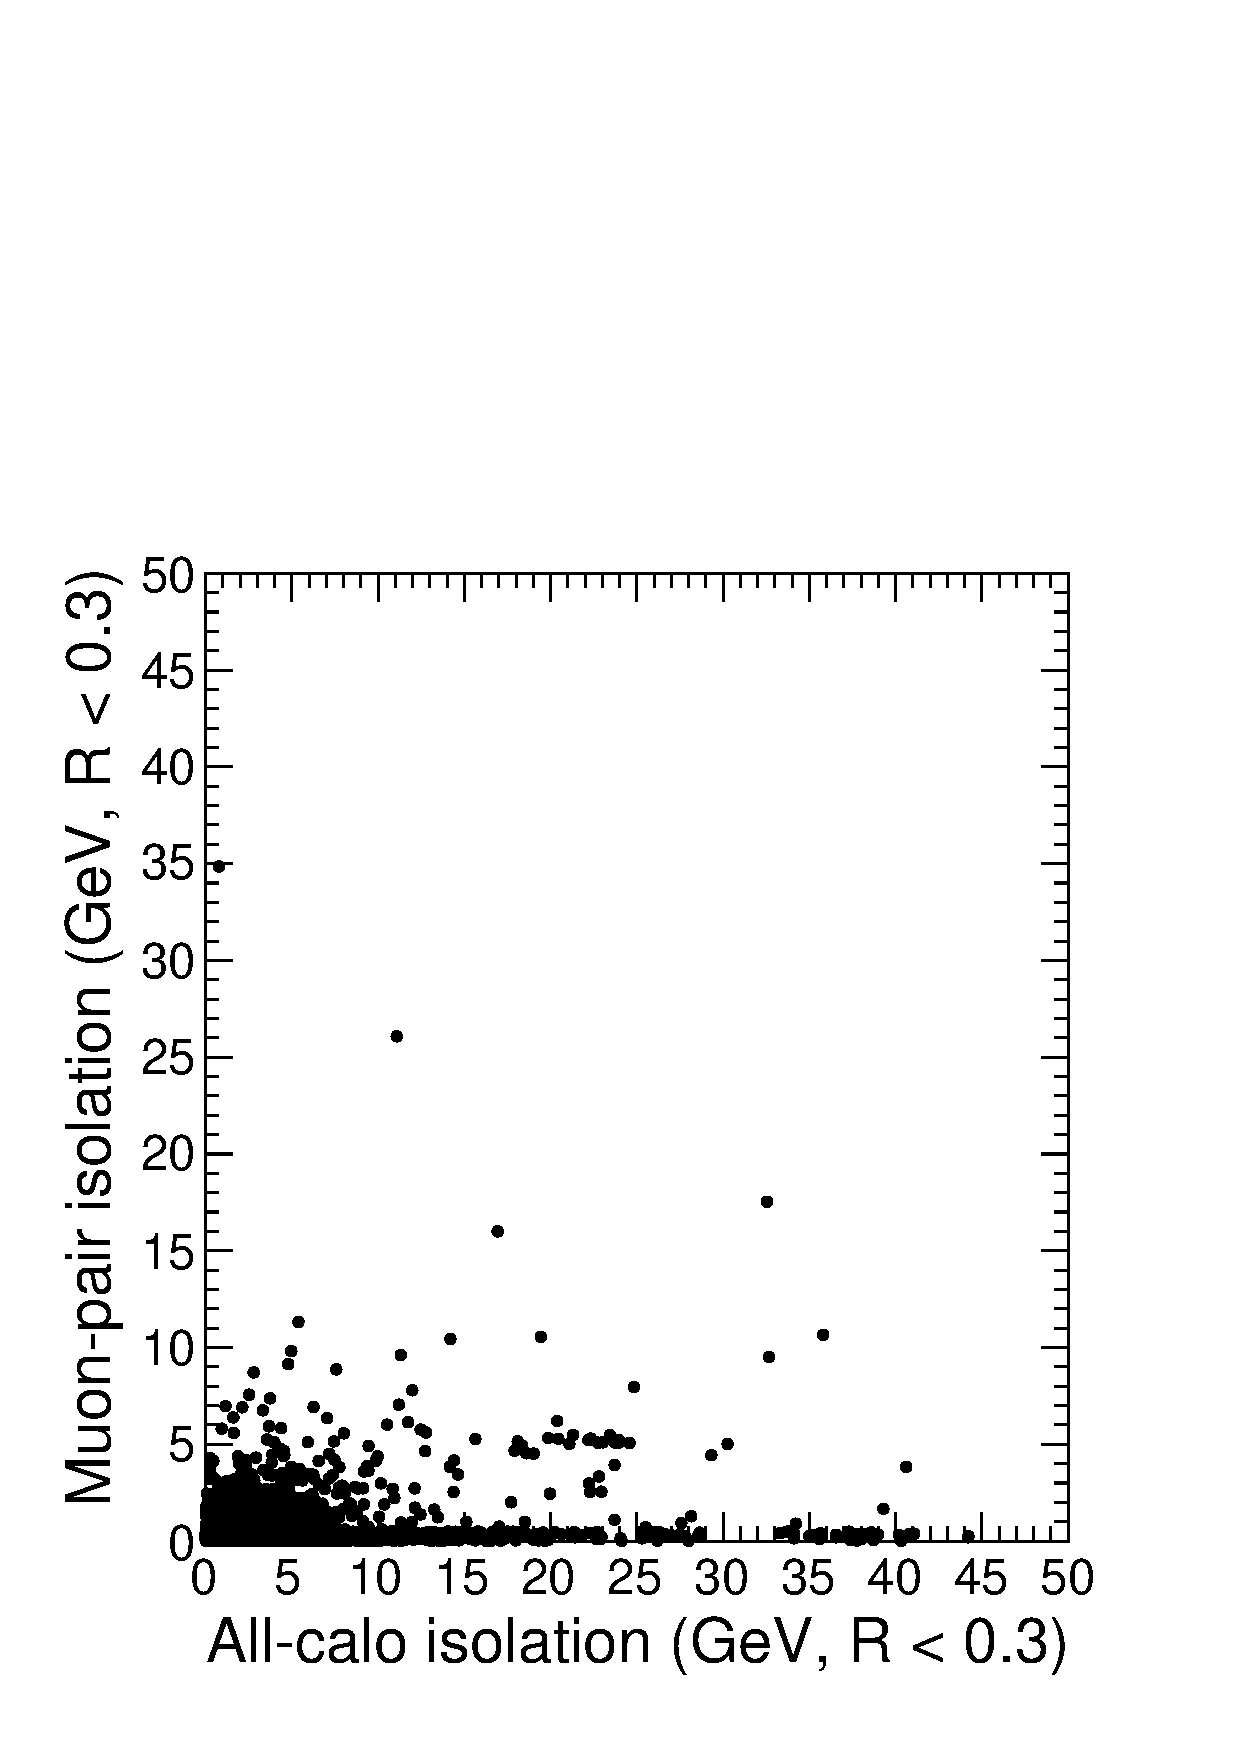
\includegraphics[width=\linewidth]{bubbleiso_vs_caloiso.pdf}
\column{0.5\linewidth}
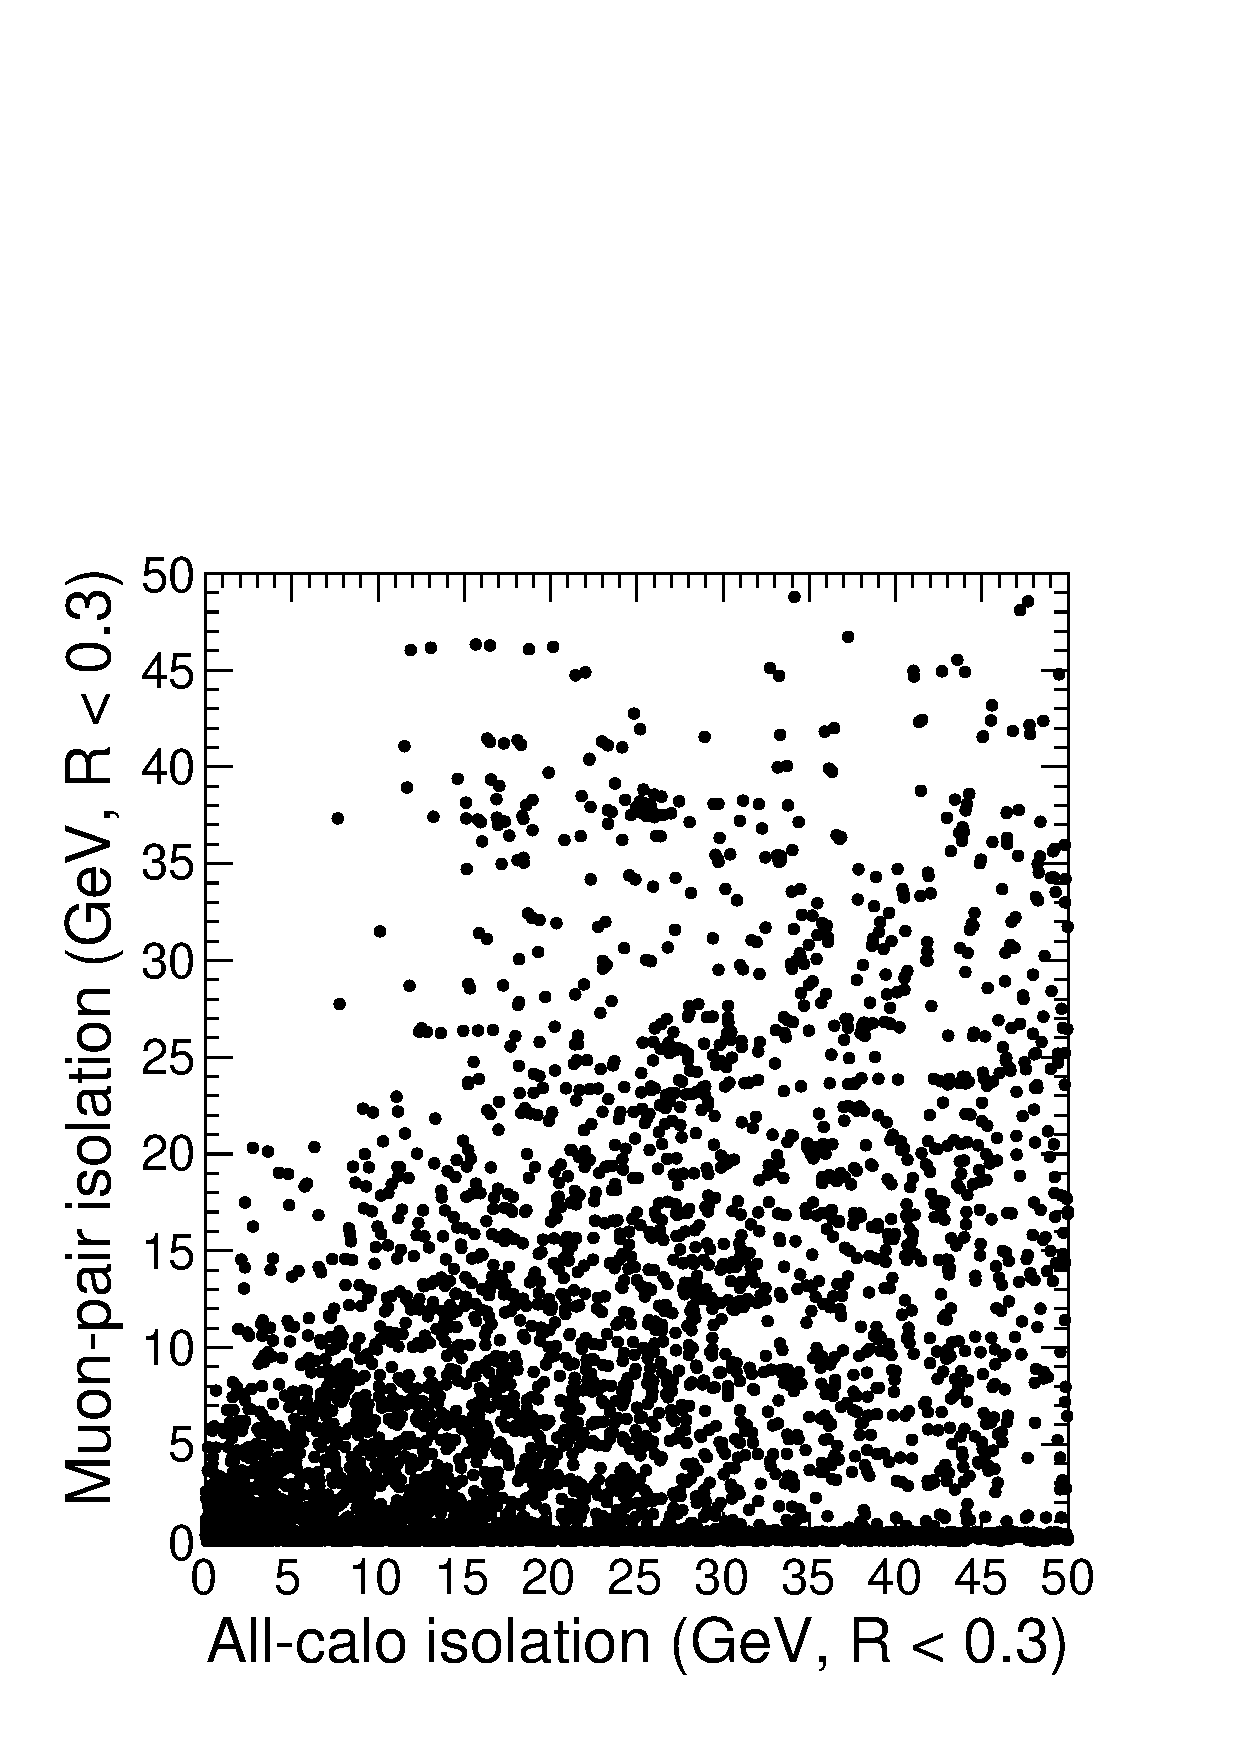
\includegraphics[width=\linewidth]{bubbleiso_vs_caloiso_background.pdf}
\end{columns}
\end{frame}

\begin{frame}
\frametitle{An idea: $X(3872)$}

\begin{itemize}
\item As we build our analysis to look for what has never before been seen ($h \to aa \to 4\mu$), we should show that we can see what's there
\item The $J/\psi$ is an obvious example, and we'll need to interact with many other groups whenever presenting anything related to $J/\psi$ (because a lot of people are looking at it)
\item Also in our sample: $X(3872) \to \pi^+\pi^- J/\psi$, four tracks with a different invariant mass topology
\item In 500~pb$^{-1}$ of 7~TeV data, we would see as many such events as the Tevatron's 8~fb$^{-1}$
\item This is an interesting state in its own right, as it may be the first example of a molecular hadron: $c\bar{c} + c\bar{c}$
\item {\tt http://arxiv1.library.cornell.edu/abs/0911.2016}
\item Unfortunately, not much discrimination power in $pp$ vs.\ $p\bar{p}$: the interesting thing about an LHC analysis is the higher cross-section, which begins to matter in 2011
\end{itemize}
\end{frame}

\begin{frame}
\frametitle{$X(3872)$ at CDF}

\begin{itemize}
\item This is what it looks like at CDF
\item {\tt www-cdf.fnal.gov/physics/preprints/cdf9700\_X\_mass.pdf}
\item 7~TeV LHC production is 15$\times$ larger, backgrounds are\ldots?
\end{itemize}

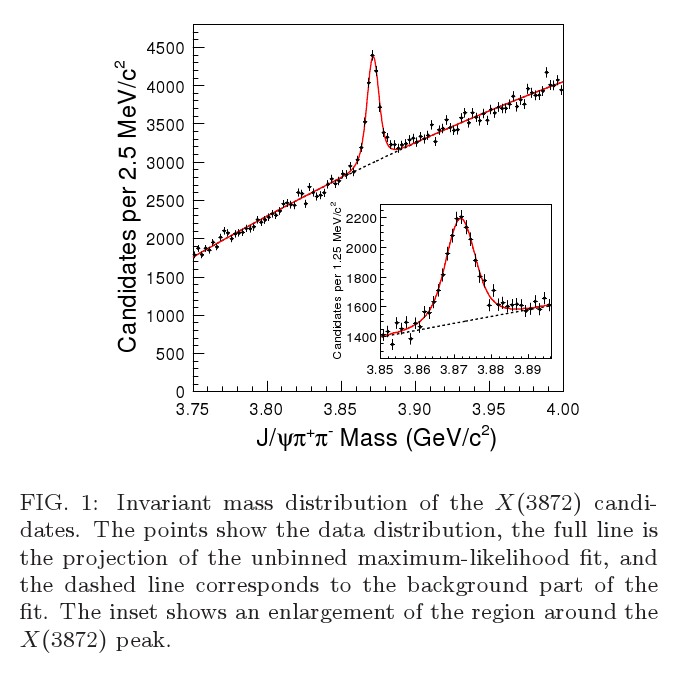
\includegraphics[width=0.5\linewidth]{cdf_x_plot.png}

\label{numpages}
\end{frame}

\end{document}
